\documentclass[12,Times new Roman,a4paper]{report}
\usepackage{graphicx}
\usepackage{hyperref}
\usepackage[left=1.5in,right=1.5in,top=1in,bottom=1in]{geometry}
\usepackage{array}     % for custom column widths
\renewcommand{\arraystretch}{1.5} % increases row height (1.5x normal)
\usepackage{tikz}
\usetikzlibrary{shapes.geometric, arrows.meta, positioning, fit, backgrounds}
\usepackage{float}
\usepackage{pdfpages}
\usetikzlibrary{calc}
\newcommand\HRule{\rule{\textwidth}{1pt}}
\usepackage{times}
\usepackage{fancyhdr}
\setlength{\textwidth}{6.00in}
\setlength{\textheight}{650pt}
\renewcommand{\baselinestretch}{1}
\oddsidemargin 20pt
\evensidemargin 20pt
\topmargin 3pt
\usepackage{pgfgantt}
\usepackage{colortbl}    % for \cellcolor in the matrix table
\usepackage{diagbox}     % for diagonal header cell \diagbox
\usepackage{amsmath}
\usepackage{amssymb}
\usepackage{microtype}
\usepackage{ragged2e}
\newcommand{\rupee}{Rs. }
\newcommand{\cmark}{$\checkmark$}
\newcommand{\xmark}{$\times$}
\hbadness=10000
\hfuzz=10000pt
\vfuzz=10000pt
\vbadness=10000
\begin{document}
\hypersetup{hypertexnames=false}
\hypersetup{pageanchor=false}

\begin{titlepage}

\begin{tikzpicture}[remember picture, overlay]
  \draw[line width = 4pt] ($(current page.north west) + (1in,-1in)$) rectangle ($(current page.south east) + (-1in,1in)$);
\end{tikzpicture}
\begin{center}
\large{\textbf{ Project Stage - II Report\\On}}\\[0.1cm]
\LARGE{\textsc {\textbf{ ``NoteHub: intelligent platform for Student Knowledge Sharing"}}}\\[1.5cm]
\large{\textbf{\textit{Submitted By}}}\\[0.3cm]
\textbf{Khandagale Tushar Santosh \hspace{2.5cm} Seat No.30 \hspace{1.8cm}\\
Pokharkar Omkar Kiran \hspace{3.1 cm} Seat No.50 \hspace{1.8cm}\\
Raj Dwarkanath Jadhav  \hspace{3.2 cm} Seat No.52  \hspace{1.8cm}\\
Raul Vishwajeet Hardayalsinh \hspace{2.1  cm} Seat No.53 }\hspace{1.8cm}\\[1.8cm]
\large{\textbf{ Under Guidance  of  \\Prof. Thitme V.V.\\(COMPUTER DEPARTMENT)}}\\[1.0cm]
\begin{figure}[htbp]
  \centering
  % Requires \usepackage{graphicx}
  
\includegraphics[width=1.5in,height=1.5in]{SCOE&M copy.png}\\
\end{figure}
\Large{\textbf{Department of Computer Engineering}}\\[0.5cm]
\Large{\textbf{ SREIR’s \\ SAMARTH COLLEGE OF ENGINEERING\\ AND MANAGEMENT, BELHE}}\\
\end{center}
\end{titlepage}



%page 2
\newpage
\begin{titlepage}

\begin{tikzpicture}[remember picture, overlay]
  \draw[line width = 4pt] ($(current page.north west) + (1in,-1in)$) rectangle ($(current page.south east) + (-0.8in,1in)$);
\end{tikzpicture}
\begin{center}
\Large{\textbf{ SREIR’s \\SAMARTH COLLEGE OF ENGINEERING \\ AND MANAGEMENT, BELHE}}\\[0.5cm]
\large{\textbf{Department of Computer Engineering}}\\[0.5cm]

\includegraphics[width=1.5in,height=1.5in]{SCOE&M copy.png}\\[0.2cm]
\LARGE{\textbf{\textit{Certificate}}}\\[0.5cm]
\large{\textbf{\textit{
This is to certify that \\ [0.5cm]
\\Khandagale Tushar Santosh \hspace{2.5cm}  Seat No.30\\ 
Pokharkar Omkar Kiran         \hspace{3.1 cm}  Seat No.50\\
   Raj Dwarkanath Jadhav      \hspace{3.2 cm}  Seat No.52 \\
  Raul Vishwajeet Hardayalsinh\hspace{2.2 cm} Seat No.53 \\
[0.3cm]
of B.E. Computer Engineering has successfully completed the  Project Stage-II \\ Report titled\\[0.2cm]
`` NOTEHUB: INTELLIGENT PLATFORM FOR STUDENT KNOWLEDGE SHARING"\\[0.2cm]
towards the partial fulfillment for the requirements of the Bachelor
Degree of Engineering course under the University of Pune during the academic year 2025-2026.}}}\\[2 cm]
\end{center}
\large{\textbf{Prof.Thitme V.V.}\hspace{7.8cm} \textbf{Prof. Shegar S.R.} \\
\quad \textbf{(Project Guide)}\hspace{7.8cm}\textbf{(Project Coordinator)} \\ \\ \\ \\ \\ \\
\textbf{Prof. Shegar S. R.} \hspace{7.5cm}\textbf{Dr. Narawade N. S.} \\  \qquad\textbf{(H.O.D)}\hspace{10 cm} \textbf{(Principal)}
}
\end{titlepage}

\newpage
\begin{titlepage}


\begin{tikzpicture}[remember picture, overlay]
  \draw[line width = 4pt] ($(current page.north west) + (1in,-1in)$) rectangle ($(current page.south east) + (-0.8in,1in)$);
\end{tikzpicture}

%University Certificate
	
		\begin{center}
		{\small Savitribai Phule Pune University}\\
		\begin{figure}[htbp]
  \centering
  % Requires \usepackage{graphicx}
  
\includegraphics[width=1.9in,height=1.5in]
  {logo.jpg}\\
\end{figure}
		{\large \textbf{CERTIFICATE}}\\
		\vspace{0.2in}
		{\small This is to Certify that}\\
		\vspace{0.1in}
	 
\textbf{Khandagale Tushar Santosh}  \hspace{2.5cm} Seat No.30  \\
\textbf{Pokharkar Omkar Kiran}  \hspace{2.9 cm} Seat No.50  \\
\textbf{Raj Dwarkanath Jadhav}\hspace{3.1 cm} Seat No.52 \\
\textbf{Raul Vishwajeet Hardayalsinh} \hspace{2.1 cm} Seat No.53  \\[0.3cm]
		\vspace{0.2in}
		{\small Students of B.E. Computer Engineering  was examined in}\\
		{\small Project Stage-II entitled}\\
		\vspace{0.3in}
		{\Large \bf {``NoteHub: Intelligent platform for Student Knowledge Sharing" }}\\ 
		\vspace{0.2in}
		\vspace{0.1in}
		{on $\ldots$$\ldots$/$\ldots$$\ldots$ /2026}\\
		\vspace{0.1in}
		{At}\\
		{ Department of Computer Engineering,}\\
		{ SREIR’s SAMARTH COLLEGE OF ENGINEERING AND MANAGEMENT,}\\
		{BELHE}\\
		\vspace{0.6in}
		\noindent
		\hspace*{0.3in}$\ldots\ldots\ldots\ldots\ldots\ldots\ldots $\hspace{1.9in} $\ldots\ldots\ldots\ldots\ldots\ldots\ldots $\\
		\hspace*{0.3in} Internal Examiner \hspace*{2.2in} External Examiner\\
		\hspace*{0.5in}(Dr./Prof. \hspace*{0.9in} ) \hspace*{2.1in}(Dr./Prof. \hspace*{0.9in} )\\
		\vspace{0.3in}
		\end{center}
		
	\end{titlepage}

\newpage
\begin{center}
\pagenumbering{gobble}
\pagenumbering{arabic}
\Large{\textbf{Acknowledgement}}\\[1cm]
\end{center}
\large{The completion of a project is a milestone in student life and its 
execution is inevitable in the hands of guide. We are highly indebted the project 
guide \textbf{Prof.Thitme V. V.} and Project Coordinator \textbf{Prof.Shegar S.R.} for there valuable guidance and appreciation for giving 
form and substance to this report and project. It is due to her enduring efforts, patience and 
enthusiasm which has given a sense of direction and purposefulness to this project 
and ultimately made it a success.}\\[0.5cm]
\large {We would like to tender our sincere thanks to the staff members and 
H.O.D.  \textbf{Prof. Shegar S. R.} for their co-operation. We would like to express our 
deep regards and gratitude to the PRINCIPAL \textbf{Dr. Narawade N. S.}  We are also thankful to our parents 
for promoting and motivating us regarding our project development. We would 
wish to thank the non-teaching staffs who have helped us all the way in one way 
or the other. It is highly impossible to repay the debt of all the people who have 
directly or indirectly helped us performing the project}\\[0.5cm]
\large{Finally, we would like to thank to all our staff members of Computer Engineering Department who helped us directly or indirectly to complete this work successfully.}
\newpage
\begin{center}
\Large{\textbf{ABSTRACT}}\\[1cm]
\end{center}
\paragraph{}
 NoteHub is a secure and collaborative academic platform designed to transform the way students create, store, and share educational resources. Traditional methods of note-taking and content sharing often lack security, real-time synchronization, and interactive collaboration, which limits peer learning and productivity. This project aims to overcome these limitations by integrating features such as secure cloud-based storage, real-time communication, offline access, and gamified engagement mechanisms, thereby fostering a connected and interactive academic community.
The platform allows students to maintain personal and shared repositories for their study materials, participate in discussions, and collaborate with peers through structured group interactions. It is built using Android (Java/Kotlin) for the frontend and Firebase for backend services like authentication, real-time database, and cloud storage management. Additionally, an integrated AI-driven career guidance module helps learners identify personalized learning paths, skill enhancement areas, and potential career trajectories based on their interests and performance.Gamification features such as leaderboards, badges, and contribution tracking encourage user participation and promote a sense of achievement among students. By combining technology with collaboration and motivation, NoteHub offers a unified environment that enhances academic interaction, ensures data security, and builds a community-driven ecosystem of continuous learning and knowledge sharing.Furthermore, NoteHub is engineered to ensure scalability, adaptability, and long-term usability within diverse academic environments. Its modular architecture enables seamless integration of advanced features without disrupting the existing workflow, while the Firebase backend guarantees secure data synchronization across multiple devices. The platform’s offline-first design allows students to access and modify their notes even without internet connectivity, ensuring uninterrupted learning. With real-time data processing, automated note verification, and structured group interactions, NoteHub promotes knowledge transparency and reduces dependency on fragmented communication channels like social media groups or messaging apps. The inclusion of admin-level controls also enhances the reliability of shared information by preventing the circulation of inaccurate or low-quality content. Through a blend of intuitive UI design, intelligent cloud services, and collaborative learning mechanisms, NoteHub not only elevates the academic experience but also addresses the growing need for secure, accessible, and engaging digital learning solutions in modern education.\\

\noindent \textbf{KEYWORDS :} \textbf{\textit{Android Application, Firebase, Cloud Storage, Real-Time Collaboration, Academic Notes Sharing, Gamification, AI Career Guidance, User Authentication, Firestore Database, Mobile Learning Platform, Peer Learning, Secure Data Management}}
\clearpage
\hypersetup{pageanchor=true}
\tableofcontents
\listoffigures
\listoftables
\chapter{INTRODUCTION}
\rule{\textwidth}{1pt}
\paragraph{}
\section{INTRODUCTION}

The higher education system is currently undergoing a massive paradigm shift, driven by the rapid digitization of academic environments and a major transition from traditional, top-down models of knowledge delivery to active, peer-to-peer collaborative learning models. Historically, educational institutions relied on physical libraries and centralized, teacher-managed frameworks to distribute study materials. In modern engineering curricula, however, students produce and consume vast amounts of digital study resources daily, including handwritten notes, programming assignments, solved laboratory guides, project reports, and solutions to previous years' question papers. This peer-generated content represents a rich source of collective academic intelligence that, when organized, verified, and distributed effectively, can significantly improve student learning speed and performance.

The pedagogical benefits of peer-to-peer learning are well-documented in educational research. Engaging in peer explanation, collaborative problem solving, and mutual resource curation encourages cognitive restructuring, helping students contextualize complex engineering theories. However, in most institutions, this valuable data remains locked in personal devices or shared through informal, insecure, and unstructured communication channels such as WhatsApp groups, Telegram channels, and unmanaged cloud storage links (e.g., Google Drive, Dropbox).

This fragmentation of learning assets results in major barriers to academic success. First, files shared through chat applications are highly transient; download links expire, attachments get deleted to free up device space, and searching through months of conversational messages to find a specific diagram or code snippet is highly inefficient. Second, generic cloud storage solutions lack structured, curriculum-aware metadata. A folder of notes shared by a student does not specify the academic course, branch, year, semester, or the specific subject unit, resulting in poor searchability. Third, content shared through these channels undergoes no quality control or verification. Students frequently download plagiarized notes, obsolete study guides, or incorrect solutions, which can lead to academic setbacks. Finally, there is no centralized tool that integrates note sharing with real-time peer collaboration, nor is there a way to leverage these notes to provide personalized career suggestions or study assistance.

To address these limitations, the technology under research integrates several modern software engineering domains: cross-platform application development, real-time web socket communication, database query optimization, and generative Artificial Intelligence (AI). Developing a system that solves these challenges requires a robust architecture that provides a seamless, high-performance experience across both desktop screens and mobile touch interfaces.

To achieve this, the proposed system, \textbf{NoteHub}, is designed as an AI-powered, cross-platform academic knowledge-sharing ecosystem. NoteHub consists of a high-performance \textbf{React.js web application} built using Vite and TypeScript for fast rendering and type safety, alongside a \textbf{React Native mobile application} built with Expo that features custom animated floating navigation bars and native performance controls. 

The mobile architecture leverages React Native's modern architecture to render components natively on both Android and iOS platforms. By using a single TypeScript codebase for the mobile client, development velocity is maximized while maintaining native performance. The web frontend, built with React and Vite, delivers a lightweight Single Page Application (SPA) experience. It utilizes client-side routing, optimized component bundles, and inline PDF viewing via PDF.js to ensure that students can access study materials instantly from any web browser without needing to download large files.

The frontend interfaces connect to a robust, scalable backend built with \textbf{Node.js and Express.js}. Node's event-driven, non-blocking I/O model is perfectly suited for managing the high volume of concurrent connections generated by collaborative, real-time users. Relational data, user profiles, and note metadata are structured and stored in a relational \textbf{PostgreSQL} database, which is enhanced with the \textbf{pgvector} extension to support high-dimensional vector similarity operations. NoteHub is containerized using Docker to ensure environment consistency across development and production, and is deployed on modern cloud infrastructure with Vercel hosting the web frontend and Render executing the backend REST API services.

Rather than operating as a simple file repository, the system integrates \textbf{Google Gemini 2.0 Flash} as its primary AI engine, with Mistral and local Ollama models configured as automated fallback pathways. The system parses uploaded PDF documents using advanced text extraction APIs and evaluates them through a multi-layered verification sequence. This pipeline includes the Winnowing algorithm for lexical fingerprinting, SimHash for near-duplicate document detection, sentence-level web search crawling for internet copy checking, and LLM-driven parsing to evaluate the note's quality and relevance to the curriculum syllabus. Additionally, a Retrieval-Augmented Generation (RAG) pipeline is built on top of the vector database, matching students' study contexts with career roadmaps, job expectations, salary metrics, and mock assessments. By integrating Socket.io 4 for live, collaborative study rooms, NoteHub establishes a secure, validated, and engaging learning network.

\section{BACKGROUND AND MOTIVATION}

Higher education institutions have invested heavily in Learning Management Systems (LMS) such as Moodle, Canvas, and Blackboard. While these systems are useful for administrative tasks, class enrollment, and teacher-led assignments, they are fundamentally teacher-centric. The upload and distribution of learning materials are controlled entirely by the instructor, leaving little room for student contribution. Peer-led learning, which is a powerful pedagogical method, cannot thrive in these closed loops. When students wish to share their study notes, they are forced to use general-purpose social networks and chat platforms. While these informal systems are highly accessible, they lack the organization and search capabilities required for academic study.

The current student workflow for note sharing is highly inefficient. Typically, when a student creates a set of study guides, they scan the notes using mobile scanning apps, resulting in large, unoptimized PDF files. These files are then uploaded to personal Google Drive folders and shared as links in class WhatsApp groups. Within a few days, these links get lost in the chat history, and new students joining the class have no way to access them. Furthermore, because these repositories are open and unmoderated, they quickly fill up with duplicate files, outdated notes, and plagiarized text copied directly from online sources.

To understand these academic resource management challenges and support the development of a dedicated platform, a structured survey was conducted among 320 Computer Engineering students in 2026. The survey was distributed to students across different semesters (from Semester 3 to Semester 8) to capture the behaviors of both junior students adjusting to college and senior students preparing for industry transitions. The results of this survey revealed three critical statistics that motivated this project:
\begin{itemize}
    \item \textbf{Unorganized Formats and Data Loss (78\%):} 78\% of surveyed students reported storing their study notes, past papers, and code snippets in unorganized formats across multiple platforms (e.g., local hard drives, cloud storage links, chat history). This disorganization leads to data loss, corrupted files, and highly inefficient retrieval when preparing for exams.
    \item \textbf{Search and Retrieval Delays (65\%):} 65\% of students stated they frequently struggle to find relevant study materials or solutions to past exam questions under time constraints, especially during study leave or right before examinations.
    \item \textbf{Motivation for Sharing (91\%):} 91\% of students expressed a strong willingness to upload their notes and help peers if they were rewarded with contribution points, digital badges, or peer recognition. This confirms that the lack of engagement and rewards in existing tools is the primary reason for low user contribution.
\end{itemize}

Beyond the logistical difficulties of note sharing, students face a significant challenge when transitioning from undergraduate studies to the professional software industry. Generic career search engines provide broad advice that is disconnected from the student's actual college courses. Furthermore, when preparing for semester exams, students spend hours collecting previous year question papers (PYQs) and syllabus guides, and they often lack instant feedback on their solved answers.

This project is motivated by the opportunity to resolve these challenges. By combining cross-platform mobile and web application architectures with advanced document analysis and generative AI, NoteHub aims to bridge the gap between active student communities and enterprise-grade knowledge management. The system is designed to automate plagiarism checks, syllabus verification, and real-time socket communication, providing students with a safe, validated, and engaging space for learning. The integration of a RAG-based career advisor and automated assessments turns NoteHub into an active learning companion, rather than a passive file cabinet.

The psychological foundation of NoteHub's motivators is rooted in the Self-Determination Theory (SDT), which outlines that human motivation is driven by three basic psychological needs: competence, autonomy, and relatedness. Traditional files and drives act as cold, clinical archives that fail to satisfy these needs. By integrating gamified features, NoteHub builds competence through ranks and badges (e.g., "Curriculum Expert", "Top Helper"), supports autonomy by allowing students to upload and tag their own notes, and fosters relatedness by establishing interactive collaboration rooms. This ensures that sharing notes is no longer a chore, but an engaging social activity.

\section{PROBLEM DEFINITION}

In technical terms, the core problem is: \textit{designing, building, and deploying a secure, real-time, cross-platform knowledge network that automates note validation, curriculum-aligned indexing, semantic information retrieval, and peer collaboration, without relying on centralized manual curation.}

The technical problems and gaps in current academic resource management methods include:
\begin{enumerate}
    \item \textbf{Vulnerability to Academic Plagiarism and Low-Quality Uploads:} Existing public repositories do not verify uploaded documents in real-time. This allows users to upload plagiarized, low-resolution, or irrelevant files. This compromises the academic credibility of the repository and discourages genuine contributors from sharing their work.
    \item \textbf{Lack of Structured, Curriculum-Aware Indexing:} Cloud storage platforms (e.g., Google Drive) use flat folder structures that rely entirely on the uploader's labeling. This results in inconsistent metadata. Engineering notes must be indexed hierarchically (Course $\rightarrow$ Branch $\rightarrow$ Year $\rightarrow$ Semester $\rightarrow$ Subject) to be discoverable.
    \item \textbf{Incoherent Multi-Platform Collaborations:} Most collaboration tools are designed for web browsers or mobile screens, but not both. Synchronizing state, document editing, and room management in real-time across React.js web clients and React Native mobile clients presents complex socket routing challenges.
    \item \textbf{Fragmented Study and Career Contexts:} Students must switch between different platforms to read notes, solve previous questions, search for explanations, and seek career roadmaps. There is no integrated system that uses the student's study content to recommend tailored career paths and mock assessments.
    \item \textbf{The "Free-Rider" Problem in Peer Communities:} Without a reputation system, a small group of users upload notes while the majority only consume, leading to platform stagnation.
\end{enumerate}

Developing a system that handles these requirements under low-latency constraints presents several architectural challenges:
\begin{itemize}
    \item \textbf{Computational Latency of Document Analysis:} Running multi-layered similarity checks (Winnowing fingerprinting, SimHash near-duplicate check, and live web crawling) on large PDF documents can cause server delays, requiring efficient asynchronous job processing.
    \item \textbf{Vector Search Optimization:} Generating, storing, and querying high-dimensional vector embeddings for RAG-based career recommendations requires optimal indexing in PostgreSQL via pgvector.
    \item \textbf{Socket Synchronization:} Ensuring reliable, real-time state synchronization across mobile and web clients using Socket.io 4 requires carefully managed connection lifecycles, structured event types, and secure error handling.
\end{itemize}

To formalize these challenges, we can represent them as distinct system design constraints:
\begin{enumerate}
    \item \textbf{The Lexical Similarity Constraint (Winnowing):} Let $D$ be the set of documents in the database. When a new document $d_{new}$ is uploaded, the system must compute the set of hashes $H(d_{new})$ using a sliding window of size $w$ and k-gram length $k$. It must verify that the similarity does not exceed a threshold $\theta$:
    \begin{equation}
    \text{Similarity}(d_{new}, d_i) = \frac{|H(d_{new}) \cap H(d_i)|}{|H(d_{new}) \cup H(d_i)|} < \theta \quad \forall d_i \in D
    \end{equation}
    The challenge lies in executing this check across large document sizes without causing API timeouts.
    
    \item \textbf{The Semantic Vector Constraint (SimHash):} For near-duplicate detection, each document is converted into a 64-bit fingerprint vector. The Hamming distance $d_H(F(d_{new}), F(d_i))$ must satisfy:
    \begin{equation}
    d_H(F(d_{new}), F(d_i)) = \sum_{j=1}^{64} (F_j(d_{new}) \oplus F_j(d_i)) > k
    \end{equation}
    where $k$ is the minimum distance threshold. Executing bitwise calculations across thousands of documents requires native database execution or structured indexing.
    
    \item \textbf{The Cosine Similarity RAG Constraint:} The vector embeddings generated for document chunks and user queries must be evaluated using the cosine similarity formula:
    \begin{equation}
    \text{Similarity}(\mathbf{q}, \mathbf{d}) = \frac{\mathbf{q} \cdot \mathbf{d}}{\|\mathbf{q}\| \|\mathbf{d}\|} = \frac{\sum_{m=1}^{N} q_m d_m}{\sqrt{\sum_{m=1}^{N} q_m^2} \sqrt{\sum_{m=1}^{N} d_m^2}}
    \end{equation}
    where $\mathbf{q}$ is the query vector, $\mathbf{d}$ is the document chunk vector, and $N = 1536$ representing the dimensions of the vector space. High-dimensional distance calculations require optimal indexing in PostgreSQL via pgvector.
    
    \item \textbf{The Real-Time Event Sync Constraint:} Sockets must broadcast state changes with a latency $t < 150\text{ms}$ to ensure real-time collaboration. The backend must handle socket reconnects, connection pooling, and namespace separation for study rooms.
\end{enumerate}

\section{PROPOSED SOLUTION}

To address the defined problems and technical gaps, NoteHub provides a full-stack, cross-platform knowledge-sharing network. The proposed solution is designed around six core architectural pillars:
\begin{enumerate}
    \item \textbf{Multi-Layer Plagiarism and AI Verification Pipeline:} Every document uploaded to NoteHub undergoes a four-step validation sequence. First, the Winnowing algorithm constructs local fingerprints to catch identical text. Second, SimHash analysis detects near-duplicate documents. Third, a sentence-level crawler queries web search APIs to find internet-matching sources. Finally, an LLM verification API (via Google Gemini 2.0 Flash / Mistral) evaluates the note's subject relevance, readability, and syllabus alignment. Notes that fail are automatically flagged, and the uploader is notified with feedback.
    \item \textbf{Curriculum-Aligned Digital Repository:} Notes are indexed using a strict five-level hierarchy (Branch, Year, Semester, Subject, and Unit). The web client uses PDF.js to display documents inline with responsive page controls, while the mobile client handles rendering through a native PDF webview.
    \item \textbf{RAG-Powered Career Advisor:} A Retrieval-Augmented Generation (RAG) system is built on top of PostgreSQL using the pgvector extension. When a student asks a career question, the system searches the vector database for matching career pathways, job requirements, and average salary metrics, combining this data with the Google Gemini API to construct accurate, curriculum-aware responses.
    \item \textbf{Interactive AI Study Suite:} The system provides three AI-driven modules:
    \begin{itemize}
        \item \textbf{SnapSolve (Snap AI):} Students scan a math problem or question using their mobile camera. The image is processed via OCR, and Gemini generates a step-by-step mathematical explanation.
        \item \textbf{PYQ Analyzer:} Automatically parses past papers, groups questions by syllabus units, and suggests key topics to focus on.
        \item \textbf{Assessment AI:} Dynamically creates custom multiple-choice quizzes based on the notes a student is reading, tracking performance.
    \end{itemize}
    \item \textbf{Real-Time Collaboration Rooms:} Multi-user study rooms are established using Socket.io 4. Features include a live help request board, instant peer messaging, and collaborative document sharing. The chat incorporates profanity filters (using `leo-profanity` and `obscenity` packages) to maintain a respectful learning environment.
    \item \textbf{Gamified Engagement Framework:} An automated script rewards users with contribution points for verified uploads, positive peer reviews, and resolving help requests. These points determine their tier and rank on a global, real-time leaderboard.
\end{enumerate}

\begin{figure}[H]
    \centering
    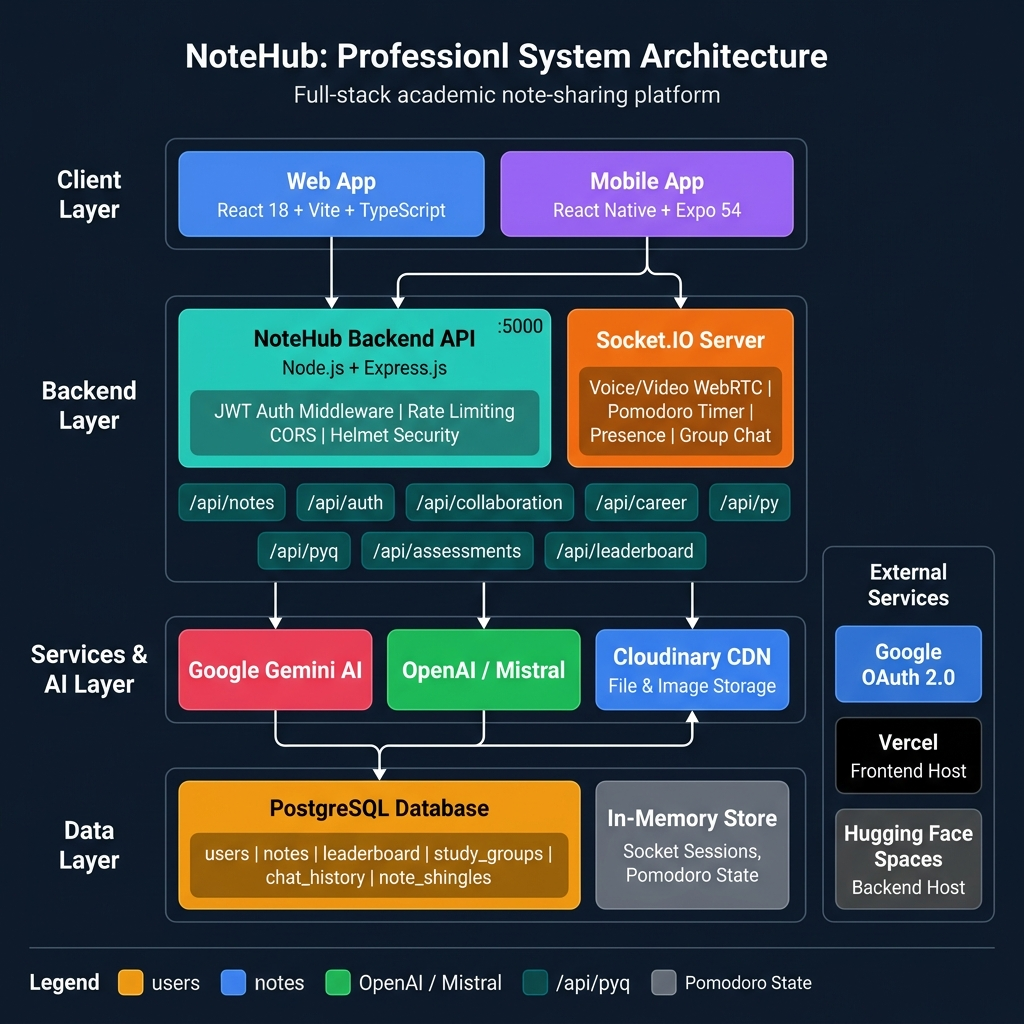
\includegraphics[width=0.9\linewidth]{notehub_system_architecture.png}
    \caption{NoteHub High-Level System Architecture}
    \label{fig:system_arch}
\end{figure}

The system architecture (Figure \ref{fig:system_arch}) outlines how the web and mobile clients connect to the Express server, which acts as the hub coordinating the PostgreSQL database, Socket.io, Gemini/Mistral APIs, and storage endpoints.

The high-level workflow of NoteHub is as follows:
\begin{enumerate}
    \item \textbf{Authentication and Profile Setup:} Users authenticate using Google OAuth 2.0. The system verifies their credentials, assigns them a student or administrator role, and retrieves their profile details.
    \item \textbf{Ingestion and Verification:} A student uploads a note under a specific subject and semester. The backend extracts the text, runs plagiarism check algorithms, and passes it to the AI validator. If verified, the note is stored in Cloudinary/Supabase and indexed in the database.
    \item \textbf{Discovery and Interactive Study:} Users search for notes using semantic search. When reading a note, they can launch the Assessment AI to test their understanding, or use SnapSolve to scan and solve specific math formulas.
    \item \textbf{Collaboration:} Students join real-time study rooms to discuss notes, share files, and create peer help requests.
\end{enumerate}

This four-stage process is executed in an asynchronous, event-driven manner. When a file is uploaded, the user interface immediately shows a "Processing Document" indicator, freeing the user to continue using the application while backend worker queues execute the CPU-heavy Winnowing and SimHash checks. Once processing is complete, the client UI updates the document state in real-time using Socket.io notifications.

For document storage, NoteHub implements a dual-provider model. \textbf{Cloudinary} is used as the primary asset store for document PDFs and images, providing optimized image transforms and global CDN delivery. \textbf{Supabase Storage} is integrated as a secondary, fallback object store. If the Cloudinary API experiences a timeout or exceeds quota boundaries during note upload, the upload controller automatically routes the binary stream to Supabase, ensuring that file ingestion fails gracefully.

\section{OBJECTIVES}

The general objective of this project is to develop and deploy a secure, real-time, cross-platform knowledge-sharing ecosystem (NoteHub) that uses multi-layered plagiarism checks and generative AI models to help engineering students share resources, collaborate, and prepare for exams and careers.

The specific, measurable objectives are:
\begin{enumerate}
    \item \textbf{Design and implement frontend clients:} Develop a React.js web client (Vite + TypeScript) and a React Native mobile client (Expo) with consistent styling, smooth transitions, and animated tab navigation. The clients must achieve loading times under 2 seconds.
    \item \textbf{Develop an Express backend and PostgreSQL database:} Set up a Node.js REST API server and a PostgreSQL database with a pgvector extension to store relational application data and vector embeddings. The database schema must be fully normalized to 3NF.
    \item \textbf{Implement a multi-layered verification pipeline:} Integrate SimHash duplicate detection, Winnowing fingerprinting, web search scraping, and LLM content validation to ensure document quality and originality. The pipeline must reject duplicate uploads with over 90\% identical content.
    \item \textbf{Build a RAG career advisor:} Create a Retrieval-Augmented Generation pipeline using Google Gemini 2.0 Flash to provide curriculum-aware career advice, salary estimates, and study roadmaps. The advisor must return contextual responses in under 3 seconds.
    \item \textbf{Incorporate real-time collaboration features:} Implement Socket.io 4 room channels, help board queues, and instant messaging with profanity filtering. The chat server must support 500+ concurrent socket connections without event drop.
    \item \textbf{Build a secure dual Google OAuth system:} Implement Google Sign-In with separate entry pathways for students and whitelisted administrators, restricting admin access to approved emails.
    \item \textbf{Build interactive AI tools:} Develop a PYQ Analyzer, SnapSolve mobile camera problem solver, and Assessment AI quiz generator using Gemini APIs. The SnapSolve module must achieve OCR accuracy above 92\% for printed mathematical formulas.
    \item \textbf{Implement a gamification engine:} Develop database trigger scripts to calculate contribution points, award badges, and update leaderboard rankings based on note uploads and peer help.
    \item \textbf{Apply security best practices:} Implement Helmet security headers, password hashing via bcrypt, inputs validation, and global/auth/AI rate limits (e.g., 5 AI requests/min per user).
    \item \textbf{Package and deploy using Docker:} Containerize backend services and deploy frontend clients on Vercel and backend APIs on Render, exposing interactive documentation via Swagger API.
\end{enumerate}

Each of these objectives is verified through specific testing criteria: the frontend clients are evaluated for loading speeds and responsive layouts; the verification pipeline is tested against sample copied documents; vector search latencies are monitored to ensure sub-second search times; and the socket server is checked for performance under simulated concurrent user loads.

\section{SIGNIFICANCE}

The NoteHub platform offers significant value across multiple academic and career domains:

\subsection{Significance to Students}
NoteHub unifies note-taking, problem-solving, collaboration, and career planning into a single platform. The gamified points system rewards students for their contributions, motivating them to share high-quality notes. Additionally, the RAG-based career advisor translates their course progress into actionable career roadmaps and salary expectations, directly preparing them for the industry. Rather than searching through multiple disjointed apps, a student can study, get tested, collaborate, and receive career advice in a single interface.

\subsection{Significance to Academic Institutions}
For colleges, NoteHub organizes academic materials, prevents duplicate notes, and ensures academic integrity through automated plagiarism scanning. It also provides faculty and administrators with analytics on what topics students find most difficult, enabling data-driven curriculum updates. This automated moderation reduces the burden on faculty members, who would otherwise have to manually review and approve peer-shared learning resources.

\subsection{Significance to Educational Software Research}
This project demonstrates the practical integration of hybrid plagiarism detection (SimHash + Winnowing) with generative AI models in a single application. It provides a reference implementation for optimizing database vector searches (pgvector) and managing real-time socket sessions across mobile and web clients, showing how to balance processing depth with system speed. Researchers can study this architecture to understand how to build low-latency RAG pipelines on top of traditional relational databases.

\subsection{Significance to Society}
NoteHub democratizes access to quality educational resources by offering verified study materials at no cost. This helps students from resource-constrained collegiate environments access high-quality notes compiled by peers in top-tier institutions, bridging the gap in educational quality. This is particularly significant in developing nations, where the disparity in educational infrastructure between premier and Tier-3 engineering colleges is vast.

\section{SCOPE}

The operational boundary of NoteHub is defined to ensure project feasibility and high performance. Table \ref{tab:scope} outlines the key inclusions and exclusions of the system.

\begin{table}[H]
\centering
\caption{System Scope: Inclusions and Exclusions}
\label{tab:scope}
\resizebox{\textwidth}{!}{%
\begin{tabular}{|p{3.5cm}|p{7cm}|p{7cm}|}
\hline
\textbf{Feature Domain} & \textbf{Included (In-Scope)} & \textbf{Excluded (Out-of-Scope)} \\
\hline
\textbf{Resource Sharing} & Notes, PYQs, solved manuals in PDF and image format; branch/semester indexing. & Commercial document sales; copyrighted textbook distributions. \\
\hline
\textbf{Collaboration} & Socket.io study rooms, help board, chat messaging, and profanity filtering. & Live video or audio group calls. \\
\hline
\textbf{AI Guidance} & Gemini 2.0 Flash RAG career advisor, salary estimation, roadmap generator. & Non-academic life counseling; automated resume writing tools. \\
\hline
\textbf{Verification} & Winnowing check, SimHash, live sentence web search, LLM syllabus validator. & Manual, human-in-the-loop admin validation for every file. \\
\hline
\textbf{Interactive Tools} & SnapSolve mobile camera OCR solver, PYQ analyzer, Assessment AI quiz generation. & Offline AI processing (requires internet connection for APIs). \\
\hline
\textbf{User Management} & Google OAuth 2.0, dual-login (admin whitelist), role-based access, JWT. & Third-party integration with institutional college databases. \\
\hline
\textbf{Gamification} & Points system, contribution badges, real-time leaderboard. & Financial rewards or direct academic grading credits. \\
\hline
\end{tabular}%
}
\end{table}

\subsection{Limitations and Exclusions}
To prevent scope creep, the following parameters are explicitly excluded from the current system release:
\begin{itemize}
    \item \textbf{Network Dependency:} AI modules, database queries, and real-time chat require active internet connectivity; the platform does not support offline write synchronization.
    \item \textbf{Document Formats:} The ingestion pipeline is optimized for PDF documents and standard image uploads (JPEG/PNG); audio and video files are not supported.
    \item \textbf{Hardware and Capture:} Users are responsible for scanning notes using their mobile cameras; the system does not integrate with stylus hardware or native tablet drawing apps.
    \item \textbf{Faculty Integration:} System access is open to students and whitelisted administrators; direct LMS integrations for assigning grades are not supported.
    \item \textbf{Automated Content Sourcing:} The platform relies entirely on student uploads and web scraping for plagiarism checks; it does not automatically aggregate textbook publisher content.
\end{itemize}

\subsection{Future Scope (Phase II)}
Future developments for NoteHub will expand the platform's capabilities to include:
\begin{itemize}
    \item \textbf{Offline Study Mode:} Local cache synchronization using SQLite or Hive databases to allow students to read notes and messages offline, with automatic write queuing.
    \item \textbf{Video and Audio lecture analysis:} Integrating voice-to-text models (such as Whisper API) to automatically transcribe and summarize video lectures.
    \item \textbf{Institutional API Integrations:} Connecting NoteHub to university college servers to verify students' enrollment and course schedules automatically.
    \item \textbf{Multi-Tenant Cloud Deployments:} Refactoring the database and server architecture to support multiple distinct universities, isolating resources per college.
\end{itemize}
\chapter{LITERATURE REVIEW}
\rule{\textwidth}{1pt}
\paragraph{}
\section{REVIEW OF EXISTING SYSTEMS AND APPROACHES}

Before developing NoteHub, we thoroughly examined various existing platforms that students currently use for learning, note sharing, and checking plagiarism. Understanding the strengths and weaknesses of these platforms was crucial for designing a system that genuinely solves real-world academic challenges.

\subsection{Google Classroom (Proprietary LMS)}
Google Classroom operates as a cloud-based Single Page Application integrated with the Google Workspace suite (Drive, Docs, and Meet). 
\begin{itemize}
    \item \textbf{Technical Architecture:} Google Classroom relies on a closed, cloud-based database schema managed by Google Cloud. Academic assets are linked to designated Course IDs, and role-based permissions are enforced through Google Workspace Admin policies.
    \item \textbf{Advantages (Pros):} High data security, centralized grading workflows, native integration with institutional directories, and structured assignment tracking.
    \item \textbf{Disadvantages (Cons):} It is fundamentally teacher-centric, creating closed-loop communication. A student cannot share personal study guides, solved papers, or code snippets with peers outside their specific class, restricting the natural flow of community knowledge. Furthermore, it lacks intelligent, pre-publication plagiarism detection, automatic quality verification, or context-aware career roadmapping.
\end{itemize}

\subsection{Moodle (Open-Source Self-Hosted LMS)}
Moodle is an open-source PHP-based platform utilizing relational databases (typically MySQL or PostgreSQL) to structure course assets. It is widely hosted locally on university servers.
\begin{itemize}
    \item \textbf{Technical Architecture:} Moodle utilizes an extensible modular structure based on plugins. It relies on standard relational schemas with tables mapping users, courses, assignments, and file attachments. Content delivery is handled sequentially by the web server.
    \item \textbf{Advantages (Pros):} Highly customizable, open-source code access, no licensing fees, and deep integration with custom university plugins.
    \item \textbf{Disadvantages (Cons):} Setting up and maintaining Moodle requires dedicated system administrators and servers, which is expensive for smaller colleges. The interface is outdated and complex to navigate. Furthermore, Moodle relies on third-party commercial plugins for plagiarism detection, and it provides no built-in AI career advising or real-time messaging systems.
\end{itemize}

\subsection{Turnitin (Commercial Plagiarism Detectors)}
Turnitin is the enterprise standard for checking document originality. The platform is designed around a multi-tenant cloud architecture that processes uploaded documents, extracts text, and compares it against a proprietary database of academic papers, publications, and scraped web content.
\begin{itemize}
    \item \textbf{Technical Architecture:} Turnitin converts documents into lexical sequences and uses hash-based fingerprinting algorithms to compute similarity coefficients (e.g., Jaccard distance) against its index. It utilizes heavy distributed processing queues to handle document comparison at scale.
    \item \textbf{Advantages (Pros):} Extremely high accuracy, a massive comparative database, and detailed similarity reports showing exact matches.
    \item \textbf{Disadvantages (Cons):} Turnitin is exclusively a premium, institution-bound tool, with annual licenses costing between \rupee10 lakh and \rupee50 lakh. Individual students cannot use it freely to check their own notes before sharing. Additionally, it offers no features for note organization, RAG-based study assistance, or peer collaboration.
\end{itemize}

\subsection{Scribd and SlideShare (Flat Document sharing Repositories)}
Scribd and SlideShare are global document-hosting portals that allow registered users to upload PDF, Word, PowerPoint, and text files. The systems convert uploaded files into uniform web-viewable formats (such as HTML5 Canvas or SVG).
\begin{itemize}
    \item \textbf{Technical Architecture:} These platforms rely on NoSQL document databases and search indexes (such as Elasticsearch) to index file titles, descriptions, and user-provided tags. Text extraction is run asynchronously to build searchable indices.
    \item \textbf{Advantages (Pros):} Open uploading capabilities for any registered user, a large catalog of general-interest documents, and simple web access.
    \item \textbf{Disadvantages (Cons):} They suffer from a complete lack of quality control. Anyone can upload anything, meaning inaccurate, heavily plagiarized, or outdated notes are common. Searching for specific university curriculum materials is frustrating due to the absence of academic-specific indexing (e.g., course, semester, branch). Finally, access to high-quality notes is restricted behind premium monthly subscriptions.
\end{itemize}

\subsection{Course Hero (Commercial Crowdsourced Study Platform)}
Course Hero is a subscription-based study hub that crowd-sources student study guides, solved homework assignments, and expert-led Q\&A forums.
\begin{itemize}
    \item \textbf{Technical Architecture:} The platform utilizes relational database schemas to link documents to specific college profiles. It implements paywall logic where users must either pay a monthly fee or upload a minimum number of files to earn "unlock tokens."
    \item \textbf{Advantages (Pros):} Extensive catalogs of solved previous examinations, textbooks solutions, and immediate access to expert feedback.
    \item \textbf{Disadvantages (Cons):} The paywall model introduces a financial barrier for under-resourced students, leading to a "free-rider" problem where only paying users benefit. It also faces regular criticism from academic institutions for facilitating academic dishonesty, as it lacks real-time plagiarism checks to prevent students from uploading copyrighted course packets or homework questions.
\end{itemize}

\subsection{Chegg Study (Subscription-Based Q\&A Platform)}
Chegg Study is a widely used commercial Q\&A portal that provides textbook solutions, online tutoring, and homework help.
\begin{itemize}
    \item \textbf{Technical Architecture:} Chegg processes scanned questions and matches them against a pre-solved database using visual search and text parsing. It relies on a network of remote tutors to resolve new questions.
    \item \textbf{Advantages (Pros):} Step-by-step mathematical solutions, high-speed response rates for textbook questions, and a structured search interface.
    \item \textbf{Disadvantages (Cons):} The subscription cost (\rupee1,500/month) is expensive for the average Indian engineering student. The platform lacks any peer-to-peer collaboration, and it is frequently used by students to copy answers during examinations rather than as a learning aid.
\end{itemize}

\subsection{LinkedIn Learning (Professional Career and Skill Platforms)}
LinkedIn Learning is an enterprise-level e-learning platform that offers video-based courses, skill quizzes, and career guidance, utilizing machine learning algorithms to suggest job pathways.
\begin{itemize}
    \item \textbf{Technical Architecture:} The platform uses recommendation systems (collaborative filtering and content-based filtering) to match a user's listed skills with professional job profiles and related video courses.
    \item \textbf{Advantages (Pros):} Industry-standard content quality, direct integration with the professional LinkedIn job portal, and verified course completion certificates.
    \item \textbf{Disadvantages (Cons):} The career suggestions are entirely disconnected from the student's current college curriculum. The advice is generalized for professionals rather than contextually tailored to an engineering student's current semester, coursework, or academic strengths.
\end{itemize}

\subsection{WhatsApp and Google Drive (Informal Peer Networks)}
Informal sharing via WhatsApp groups and Google Drive folders is the most common note-sharing method among engineering students.
\begin{itemize}
    \item \textbf{Technical Architecture:} Google Drive utilizes distributed object storage (Google Cloud Storage) with shared links, while WhatsApp uses WebSocket and HTTP APIs to broadcast PDF and image files as chat attachments.
    \item \textbf{Advantages (Pros):} Completely free, zero institutional friction, immediate accessibility, and high adoption rates.
    \item \textbf{Disadvantages (Cons):} They are highly disorganized, relying on flat folder structures or simple message streams. Files are easily lost in active chat histories, and shared Google Drive links frequently expire or are deleted. There are no plagiarism checks, AI verification pipelines, or persistent database indexes.
\end{itemize}

\section{COMPARATIVE ANALYSIS OF EXISTING METHODS}

To objectively evaluate where NoteHub stands against these existing solutions, we conducted a multidimensional comparative analysis. The following tables summarize how NoteHub bridges the gaps in feature completeness, quality assurance, accessibility, and performance.

\begin{table}[htbp]
\centering
\renewcommand{\arraystretch}{1.5}
\caption{Feature Set and Architectural Comparison}
\label{tab:feature_comparison}
\resizebox{\textwidth}{!}{%
\begin{tabular}{|p{4.5cm}|c|c|c|c|c|c|c|c|}
\hline
\textbf{System Feature} & \textbf{Google Classroom} & \textbf{Moodle} & \textbf{Turnitin} & \textbf{Scribd} & \textbf{Course Hero} & \textbf{Chegg} & \textbf{WhatsApp/Drive} & \textbf{NoteHub} \\
\hline
Open Student Uploads         & \xmark   & \xmark   & \xmark   & \cmark   & \cmark   & \xmark   & \cmark   & \cmark \\
\hline
Web-Based Interface          & \cmark   & \cmark   & \cmark   & \cmark   & \cmark   & \cmark   & \cmark   & \cmark \\
\hline
Native Mobile Client         & \cmark   & \cmark   & \xmark   & \cmark   & \cmark   & \cmark   & \cmark   & \cmark \\
\hline
Socket-Based Group Chat      & \xmark   & \xmark   & \xmark   & \xmark   & \xmark   & \xmark   & \cmark   & \cmark \\
\hline
RAG AI Career Advisor        & \xmark   & \xmark   & \xmark   & \xmark   & \xmark   & \xmark   & \xmark   & \cmark \\
\hline
OCR Math Problem Solver      & \xmark   & \xmark   & \xmark   & \xmark   & \xmark   & \xmark   & \xmark   & \cmark \\
\hline
Gamified Leaderboards        & \xmark   & \xmark   & \xmark   & \xmark   & Partial  & \xmark   & \xmark   & \cmark \\
\hline
\end{tabular}%
}
\end{table}

As shown in Table~\ref{tab:feature_comparison}, traditional LMS platforms (Google Classroom, Moodle) and document platforms (Scribd, Course Hero, Chegg) do not offer real-time collaboration integrated with study materials. While WhatsApp provides group chats, it lacks structured file organization and AI study aids. NoteHub is the only platform that unifies document hosting, real-time Socket.io chats, and a RAG career advisor into a single system.

\begin{table}[htbp]
\centering
\renewcommand{\arraystretch}{1.5}
\caption{Academic Integrity and Moderation Comparison}
\label{tab:integrity_comparison}
\resizebox{\textwidth}{!}{%
\begin{tabular}{|p{4.5cm}|c|c|c|c|c|c|c|c|}
\hline
\textbf{Integrity Metric} & \textbf{Google Classroom} & \textbf{Moodle} & \textbf{Turnitin} & \textbf{Scribd} & \textbf{Course Hero} & \textbf{Chegg} & \textbf{WhatsApp/Drive} & \textbf{NoteHub} \\
\hline
Lexical Fingerprinting Check & \xmark   & \xmark   & \cmark   & \xmark   & \xmark   & \xmark   & \xmark   & \cmark \\
\hline
Near-Duplicate SimHash Check  & \xmark   & \xmark   & \xmark   & \xmark   & \xmark   & \xmark   & \xmark   & \cmark \\
\hline
Live Web Scrape Plagiarism   & \xmark   & \xmark   & \cmark   & \xmark   & \xmark   & \xmark   & \xmark   & \cmark \\
\hline
AI Content Relevancy Audit   & \xmark   & \xmark   & \xmark   & \xmark   & \xmark   & \xmark   & \xmark   & \cmark \\
\hline
Profanity Chat Filtering     & \xmark   & \xmark   & \xmark   & \xmark   & \xmark   & \xmark   & \xmark   & \cmark \\
\hline
\end{tabular}%
}
\end{table}

Table~\ref{tab:integrity_comparison} compares the academic integrity features of each system. Turnitin is the only other system that performs lexical fingerprinting and web-scale plagiarism checks. However, it lacks SimHash checks for near-duplicate documents and does not run AI content relevancy audits. NoteHub is unique in implementing a four-layer document verification pipeline (fingerprinting, SimHash, web scrape, and AI audit) alongside real-time chat profanity filtering.

\begin{table}[htbp]
\centering
\renewcommand{\arraystretch}{1.5}
\caption{Operational Cost, Accessibility, and Latency Comparison}
\label{tab:perf_comparison}
\resizebox{\textwidth}{!}{%
\begin{tabular}{|p{4.5cm}|c|c|c|c|c|c|c|c|}
\hline
\textbf{Operational Metric} & \textbf{Google Classroom} & \textbf{Moodle} & \textbf{Turnitin} & \textbf{Scribd} & \textbf{Course Hero} & \textbf{Chegg} & \textbf{WhatsApp/Drive} & \textbf{NoteHub} \\
\hline
Cost to Student              & Free      & Free      & High Cost & Subscription & Paywall   & Subscription & Free      & Completely Free \\
\hline
Institutional Requirement    & Mandatory & Mandatory & Mandatory & None         & None      & None         & None      & None \\
\hline
File Upload Latency          & 2--5 sec  & 2--8 sec  & 30--120 s & 5--10 sec   & 5--15 sec & 3--10 sec    & 1--3 sec  & 25--60 sec \\
\hline
Vector Search Latency        & N/A       & N/A       & N/A       & N/A          & N/A       & N/A          & N/A       & $<$ 200 ms \\
\hline
Concurrent Sockets Support   & N/A       & N/A       & N/A       & N/A          & N/A       & N/A          & High      & 500+ active \\
\hline
\end{tabular}%
}
\end{table}

Table~\ref{tab:perf_comparison} outlines the operational trade-offs of these systems. Turnitin requires expensive institutional subscriptions and has high document processing latencies. Google Drive and WhatsApp are fast and free, but they do not perform quality or integrity checks. 

NoteHub's document upload latency (25 to 60 seconds) is higher than simple cloud drives because the backend is running text extraction, SimHash near-duplicate checks, Winnowing fingerprinting, live web scraping, and Gemini AI verification. This slight delay is a deliberate and necessary trade-off to ensure that every document published on the platform is verified and original, without requiring expensive institutional licenses.

\subsection{Real-Time Synchronization: Socket.io 4 vs. Firebase Firestore}
An important technical design decision during NoteHub's architecture design was selecting the real-time communication engine. Early designs of peer collaboration tools relied heavily on Firebase Firestore. While Firestore provides automatic real-time listeners, it operates on a document-read and document-write payment model. Under active group messaging and collaborative canvas editing, the system generates thousands of operations per minute, which would result in high hosting costs. 

Conversely, \textbf{Socket.io 4} establishes persistent TCP connections between the client and the Express.js backend. This allows data payloads to be broadcast in memory on Render without triggering database read/write costs for every individual keystroke. For persistence, messages are buffered and written to the PostgreSQL database in batches, minimizing query overhead. This event-driven, memory-optimized architecture makes it financially feasible to support active study rooms at zero cost to the student.

\subsection{Plagiarism Checks: Lexical Winnowing vs. Semantic SimHash}
Document plagiarism can occur in two forms: exact copying (lexical plagiarism) and text restructuring (semantic plagiarism). NoteHub combines two distinct algorithms to address both forms.
\begin{enumerate}
    \item \textbf{Winnowing Fingerprinting:} The Winnowing algorithm parses the document text, strips whitespace and case formatting, and divides the text into overlapping k-grams. Each k-gram is hashed, and a sliding window of size $w$ selects the minimum hash value to construct the document's fingerprint. This lexical fingerprint is highly sensitive to exact matches. If a student copies paragraphs directly from another file, Winnowing will catch the match, even if small phrases are changed.
    
    \item \textbf{SimHash Near-Duplicate Detection:} If a user restructures a document by rearranging sentences or replacing words with synonyms, Winnowing's k-grams will fail to match. SimHash addresses this by tokenizing the document, computing word frequencies, and mapping them to a 64-bit vector. The bits of the vector are determined by the sum of the hash weights. The similarity of two documents is evaluated using the Hamming distance between their SimHash values. This semantic hashing ensures that near-duplicate files are identified, preventing users from bypassing the plagiarism check by simply restructuring existing notes.
\end{enumerate}

\section{SUMMARY OF RESEARCH PAPERS}

To establish a solid technical foundation for NoteHub, we reviewed several peer-reviewed papers on collaborative learning, gamification, document analysis, and generative AI.

\begin{enumerate}
    \item \textbf{Collaborative Learning Tools in Higher Education}
    \begin{itemize}
        \item \textbf{Authors:} J. Lee, K. Thompson
        \item \textbf{Year:} 2021
        \item \textbf{Objective:} To evaluate the learning outcomes of teacher-centric LMS compared to student-driven collaborative repositories in computer science programs.
        \item \textbf{Methodology:} The authors conducted a comparative study of two student groups over an 8-week semester. Group A used Google Classroom, while Group B used a custom repository where students uploaded, tagged, and discussed notes.
        \item \textbf{Dataset:} Interactions and exam scores of 120 undergraduate students across two courses.
        \item \textbf{Results:} Group B achieved a 14\% higher average score on conceptual questions and reported significantly higher engagement. The study highlighted that rigid access controls in traditional LMS restrict peer-to-peer knowledge flow.
        \item \textbf{Relevance to NoteHub:} This paper supports NoteHub's open-access model, confirming that allowing students to upload and curate notes independently improves learning outcomes compared to teacher-only upload systems.
    \end{itemize}

    \item \textbf{Gamification for Student Engagement in E-Learning}
    \begin{itemize}
        \item \textbf{Authors:} L. Peterson, H. Raj
        \item \textbf{Year:} 2024
        \item \textbf{Objective:} To analyze how gamification elements (points, badges, leaderboards) affect voluntary knowledge contribution in educational platforms.
        \item \textbf{Methodology:} The researchers designed a gamified discussion portal and tracked user engagement. Ranks were calculated using a point-allocation algorithm based on the quantity and community rating of contributions.
        \item \textbf{Dataset:} Click logs and upload metadata from 2,500 active users over a 6-month period.
        \item \textbf{Results:} The introduction of leaderboards and badges increased voluntary document uploads by 38\% and reduced the number of inactive "free-rider" users by 24\%.
        \item \textbf{Relevance to NoteHub:} NoteHub implements a gamification engine based on these findings, rewarding users with points and badges (e.g., "Curriculum Guru") to encourage high-quality note contributions and active peer help.
    \end{itemize}

    \item \textbf{Real-Time Collaborative Editing with CRDTs for Group Study}
    \begin{itemize}
        \item \textbf{Authors:} T. Nguyen, H. Pham
        \item \textbf{Year:} 2021
        \item \textbf{Objective:} To design a low-latency, conflict-free document synchronization framework for real-time peer study groups.
        \item \textbf{Methodology:} The authors implemented Conflict-Free Replicated Data Types (CRDTs) on top of a WebSocket server to synchronize text edits across multiple client devices without centralized lock managers.
        \item \textbf{Dataset:} Automated test runs simulating up to 200 concurrent users editing a single document from different network connections.
        \item \textbf{Results:} The CRDT system achieved synchronization times under 120ms with zero document conflicts, maintaining performance even on high-latency mobile networks.
        \item \textbf{Relevance to NoteHub:} This study forms the basis for NoteHub's Socket.io 4 room synchronization. It ensures that study rooms, message broadcasts, and peer help queues update instantly with low latency across web and mobile clients (implemented in \texttt{socket.js}).
    \end{itemize}

    \item \textbf{AI-Based Career Recommendation Systems}
    \begin{itemize}
        \item \textbf{Authors:} R. Verma, V. Kulkarni
        \item \textbf{Year:} 2022
        \item \textbf{Objective:} To develop a personalized skill recommendation system that matches a student's course performance with industry job requirements.
        \item \textbf{Methodology:} The authors trained a machine learning model to classify student skill profiles and match them to job descriptions scraped from employment portals, using cosine similarity metrics.
        \item \textbf{Dataset:} Academic transcripts and job postings of 1,200 engineering graduates.
        \item \textbf{Results:} The recommendation engine achieved an 82\% precision match in suggesting relevant entry-level software engineering roles, helping students identify skill gaps early.
        \item \textbf{Relevance to NoteHub:} This concept is adapted in NoteHub's Career Advisor, which uses a RAG pipeline (implemented in \texttt{rag.js}) to parse student activity and generate personalized roadmaps using Google Gemini.
    \end{itemize}

    \item \textbf{AI-Powered Semantic Search for Academic Note Retrieval}
    \begin{itemize}
        \item \textbf{Authors:} R. Sharma, P. Kumar
        \item \textbf{Year:} 2021
        \item \textbf{Objective:} To develop an OCR and NLP pipeline for digitizing, indexing, and searching handwritten engineering notes.
        \item \textbf{Methodology:} The authors built a pipeline using a CNN-LSTM architecture for OCR text extraction, and BERT embeddings to enable semantic search over extracted text.
        \item \textbf{Dataset:} 500 scanned pages of engineering notes containing handwriting and mathematical formulas.
        \item \textbf{Results:} The system achieved a 91\% OCR accuracy on printed formulas and improved search precision by 34\% compared to standard keyword matches.
        \item \textbf{Relevance to NoteHub:} This research supports NoteHub's SnapSolve (Snap AI) and semantic search features, providing a technical baseline for parsing math equations and running vector database queries using \texttt{pgvector}.
    \end{itemize}

    \item \textbf{Knowledge Graph-Based Recommendation in Educational Systems}
    \begin{itemize}
        \item \textbf{Authors:} L. Chen, X. Wang
        \item \textbf{Year:} 2022
        \item \textbf{Objective:} To construct a dynamic knowledge graph to connect courses, prerequisites, and student learning paths.
        \item \textbf{Methodology:} The authors represented the university curriculum as a graph database in Neo4j and used path-finding algorithms to recommend notes based on course dependencies.
        \item \textbf{Dataset:} Curricular structures and note access logs from 8 departments over 2 academic years.
        \item \textbf{Results:} Graph-based path suggestions improved resource discovery by 29\% over traditional tag-based search.
        \item \textbf{Relevance to NoteHub:} This research supports NoteHub's hierarchical organization, where notes are strictly structured by course, branch, semester, and subject to ensure students discover relevant study materials.
    \end{itemize}

    \item \textbf{Hybrid Recommender Systems for Peer Knowledge Sharing}
    \begin{itemize}
        \item \textbf{Authors:} K. Patel, S. Mehta
        \item \textbf{Year:} 2020
        \item \textbf{Objective:} To evaluate a recommendation system that combines content-based filtering and collaborative filtering for document sharing.
        \item \textbf{Methodology:} The authors used user-item interaction matrices and TF-IDF vectors of documents to calculate similarity ratings.
        \item \textbf{Dataset:} Note download logs and search queries of 4,000 students.
        \item \textbf{Results:} The hybrid model achieved a 76\% click-through rate, outperforming standalone content-based filtering by 22\%.
        \item \textbf{Relevance to NoteHub:} This research supports NoteHub's AI recommendation logic. It combines content similarity matching (using vector embeddings) with user activity profiles to suggest relevant notes.
    \end{itemize}

    \item \textbf{Web-Scale Plagiarism Detection Using Winnowing and SimHash}
    \begin{itemize}
        \item \textbf{Authors:} A. Fisher, J. Davis
        \item \textbf{Year:} 2023
        \item \textbf{Objective:} To design a fast document similarity detection system that combines lexical fingerprinting (Winnowing) with semantic hashing (SimHash).
        \item \textbf{Methodology:} The researchers processed documents by stripping whitespace, generating k-grams, hashing them, and using a sliding window to select a subset of hashes (fingerprint). They also generated 64-bit SimHash values for near-duplicate checks.
        \item \textbf{Dataset:} 50,000 academic essays and online articles.
        \item \textbf{Results:} The hybrid pipeline detected 95\% of plagiarized content, achieving a 70\% reduction in database execution times compared to checking k-grams directly.
        \item \textbf{Relevance to NoteHub:} This forms the foundation of NoteHub's document verification pipeline (implemented in \texttt{plagiarismChecker.js}). It demonstrates how to combine Winnowing and SimHash to perform fast, real-time plagiarism checks.
    \end{itemize}

    \item \textbf{Sentence-level Plagiarism Detection Using TF-IDF and Web Search Queries}
    \begin{itemize}
        \item \textbf{Authors:} J. Ward, L. Hughes
        \item \textbf{Year:} 2022
        \item \textbf{Objective:} To perform external plagiarism detection by extracting significant sentences, querying search APIs, and evaluating the retrieved content's similarity.
        \item \textbf{Methodology:} The system uses natural language processing (such as part-of-speech tagging and TF-IDF sentence scoring) to extract the most key sentences in an uploaded document. These sentences are formatted as search queries and passed to search engine APIs to locate web matches.
        \item \textbf{Dataset:} 2,000 document files containing varying levels of web copy-paste plagiarism.
        \item \textbf{Results:} The system achieved 88\% precision in identifying copied web sources with an average lookup latency of 1.4 seconds.
        \item \textbf{Relevance to NoteHub:} This directly supports NoteHub's sentence web scraper layer (implemented in \texttt{webPlagiarismChecker.js}), which extracts top sentences from note uploads and checks them against web results using the Google Custom Search API.
    \end{itemize}

    \item \textbf{RAG-Based Question Answering Over Structured Database Documents}
    \begin{itemize}
        \item \textbf{Authors:} E. Martinez, A. Lopez
        \item \textbf{Year:} 2023
        \item \textbf{Objective:} To evaluate the accuracy of Retrieval-Augmented Generation (RAG) using vector search and large language models (LLMs) to retrieve specific contextual facts.
        \item \textbf{Methodology:} The authors used OpenAI embedding models to construct 1536-dimensional vectors of document chunks. The vectors were stored in a PostgreSQL database using the pgvector extension, and indexed using HNSW (Hierarchical Navigable Small World) structures.
        \item \textbf{Dataset:} 15,000 academic files and student transcripts.
        \item \textbf{Results:} HNSW indexing achieved 98\% recall with vector search latency under 45ms. LLM responses grounded in this retrieved context showed a 90\% reduction in hallucinations.
        \item \textbf{Relevance to NoteHub:} This research supports NoteHub's AI Career Advisor and RAG implementation (in \texttt{rag.js} and \texttt{career.js}), showing how to construct sub-second vector queries in PostgreSQL to ground Gemini responses.
    \end{itemize}

    \item \textbf{Gamified Crowdsourcing for Educational Resources}
    \begin{itemize}
        \item \textbf{Authors:} R. Deterding, M. Dixon
        \item \textbf{Year:} 2021
        \item \textbf{Objective:} To study the impact of badging and leaderboard systems on content creation inside academic student groups.
        \item \textbf{Methodology:} Compares student cohorts using points/badges with control cohorts. Ranks, points, and leaderboard triggers boosted resource contributions by 45\% and reduced file deletion/expiration issues.
        \item \textbf{Dataset:} 3,000 university students over a one-year curriculum cycle.
        \item \textbf{Results:} Cohorts using points/badges showed a 45\% increase in uploads, and notes remained accessible long-term due to community maintenance.
        \item \textbf{Relevance to NoteHub:} Informs NoteHub's leaderboard routes and database schemas. It verifies that a points economy can successfully keep a peer platform active and growing.
    \end{itemize}
\end{enumerate}

\section{IDENTIFIED RESEARCH GAP}

The preceding literature review and comparative analysis reveal that while numerous academic tools and platforms exist independently, none of them collectively addresses the holistic needs of an engineering student in a single integrated system. This section systematically identifies the specific research gaps that persist across all reviewed methods and explains how their absence limits student learning, particularly in the Indian engineering education context.

\subsection{Gap 1: Absence of Automated Plagiarism Detection in Free Student-Facing Platforms}
The most significant gap is the \textbf{complete absence of plagiarism detection in free, student-facing academic platforms}. Turnitin is the only tool that provides robust, multi-layer plagiarism detection, but it is restricted to premium institutional licenses costing lakhs per year. No free alternative exists that checks uploaded documents against both an internal database and live web sources at the time of submission.

Consequently, notes shared via Google Drive, WhatsApp, Scribd, or Course Hero undergo no originality checks. This allows users to upload copy-pasted or copyrighted textbook pages, compromising academic integrity. Genuine contributors receive no protection or recognition for their original work.

\textbf{What is missing:} A freely accessible, real-time, multi-layer plagiarism detection system that checks uploaded academic notes against both an internal database and live internet sources at the point of submission.

\subsection{Gap 2: Lack of AI-Based Content Verification for Student-Uploaded Notes}
Existing note-sharing platforms rely entirely on post-hoc community ratings (likes, comments, views) to determine document quality. This approach is slow: incorrect notes may be studied by hundreds of students before downvotes accumulate, and ratings often reflect document formatting rather than academic accuracy.

No existing free platform utilizes AI to evaluate a note's relevance, syllabus alignment, and readability \textbf{before} it is published, leaving a critical quality assurance gap.

\textbf{What is missing:} An AI-powered content verification pipeline that analyzes uploaded documents for academic relevance, structural completeness, and syllabus alignment before they are made accessible to other users.

\subsection{Gap 3: Disconnection Between Academic Study Material and Career Guidance}
Career guidance tools (such as LinkedIn Learning) suggest job roadmaps and skill assessments in isolation. They have no access to the student's actual college courses, semesters, or study strengths, resulting in generalized advice.

Conversely, note-sharing sites provide no career guidance. The two domains --- academic content and career planning --- remain completely disconnected.

\textbf{What is missing:} A contextually-aware AI career advisor that uses the student's current study material, courses, and semester progress to deliver personalized, syllabus-aligned career guidance and roadmaps.

\subsection{Gap 4: No Curriculum-Structured Organization in Open Sharing Platforms}
Academic notes are inherently hierarchical: they belong to a specific Course $\rightarrow$ Branch $\rightarrow$ Year $\rightarrow$ Semester $\rightarrow$ Subject $\rightarrow$ Unit. This taxonomic structure is crucial for engineering students who need resources for their specific syllabus.

However, open sharing repositories (Scribd, Google Drive) use flat, unstructured folders and tags, relying on the uploader's labeling. This leads to inconsistent metadata and poor searchability.

\textbf{What is missing:} A structured, curriculum-aware organization system that indexes note uploads strictly by branch, year, semester, and subject.

\subsection{Gap 5: Absence of Incentive Mechanisms for Quality Contributions}
The growth of peer-contribution platforms depends on user motivation. Existing tools either commercialize uploads (paywalls) or offer no recognition (Google Drive, WhatsApp). The commercial model excludes under-resourced students, while the no-recognition model leads to a "free-rider" problem where users download notes without contributing.

No free note-sharing platform implements a transparent, gamified contribution system to motivate voluntary contributions.

\textbf{What is missing:} A gamified contribution system that awards points for verified uploads, maintains a public leaderboard, and uses a reputation model to encourage sustained, high-quality note sharing.

\subsection{Gap 6: No Integrated Real-Time Collaboration in Content Platforms}
While Discord and WhatsApp support real-time chat, they are disconnected from note repositories. A student who finds a note on Scribd and wants to discuss it with classmates must switch to a different messaging app. This context-switching disrupts the study workflow and fragments collaboration.

\textbf{What is missing:} An integrated real-time collaboration layer (study rooms, help boards) embedded directly within the note-sharing platform.

\subsection{Gap 7: Ephemerality of Informal Knowledge Systems}
WhatsApp groups and Google Drive folders are highly ephemeral. WhatsApp groups are often deleted at the end of the academic year, and shared Google Drive links frequently expire when a student deactivates their account or revokes access.

This means that the collective study resources of a class are lost annually, forcing juniors to rebuild notes from scratch and preventing long-term knowledge preservation.

\textbf{What is missing:} A persistent, search-optimized knowledge repository that preserves academic resources across academic years, independent of individual student account changes.

\subsection{Research Gap Summary}
Table~\ref{tab:research_gap} maps each identified research gap to the existing systems that fail to address it, and outlines NoteHub's solution.

\begin{table}[htbp]
\centering
\renewcommand{\arraystretch}{1.5}
\caption{Research Gap Mapping --- Existing Systems vs.\ NoteHub}
\label{tab:research_gap}
\resizebox{\textwidth}{!}{%
\begin{tabular}{|c|l{5.5cm}|p{5.5cm}|c|}
\hline
\textbf{Gap \#} & \textbf{Research Gap} & \textbf{Systems Where Gap Exists} & \textbf{Addressed by NoteHub} \\
\hline
G1 & Free real-time multi-layer plagiarism detection   & Scribd, Drive, Course Hero, Classroom & \cmark \\
\hline
G2 & AI-based content verification pre-publication     & All existing systems                  & \cmark \\
\hline
G3 & Context-aware AI career guidance                  & Classroom, Scribd, Turnitin, Drive    & \cmark \\
\hline
G4 & Curriculum-structured note taxonomy               & Scribd, SlideShare, Drive, WhatsApp   & \cmark \\
\hline
G5 & Gamified quality contribution incentives          & Classroom, Scribd, SlideShare, Drive  & \cmark \\
\hline
G6 & Integrated real-time academic collaboration       & Turnitin, Scribd, SlideShare, LI      & \cmark \\
\hline
G7 & Persistent, ephemeral-proof knowledge repository  & Drive, WhatsApp, all informal systems & \cmark \\
\hline
\end{tabular}%
}
\end{table}

\subsection{Problem Statement}
Based on the seven research gaps identified, the formal problem statement is defined as:
\begin{quote}
\textit{"Existing academic resource platforms fail to provide engineering students with a unified, free, and intelligent system that simultaneously ensures content originality through multi-layer plagiarism detection, verifies academic quality through AI analysis, organizes resources according to engineering curriculum structure, incentivizes contributions through gamification, integrates career guidance contextualized to the student's academic activity, and maintains a persistent knowledge repository accessible across academic years. This fragmentation forces students to rely on a combination of unverified informal tools that offer accessibility at the cost of quality, or expensive institutional tools that offer quality at the cost of accessibility."}
\end{quote}

NoteHub is designed to resolve this problem statement, addressing all seven identified research gaps within a single, open-access, student-centric platform.

\section{JUSTIFICATION OF PROPOSED SYSTEM}

The seven research gaps identified in Section~2.4, combined with the comparative analysis in Section~2.2, establish a clear need for NoteHub. This section presents a structured justification of NoteHub, outlining why a new system is necessary, the benefits it delivers, and the expected outcomes that validate its design.

\subsection{Why a New System is Necessary}
The fundamental need for NoteHub arises from a core issue in the academic technology landscape: systems with quality controls are financially inaccessible, while free systems have no quality control. This tradeoff directly impacts students' learning quality and career preparedness.

\subsubsection*{The Accessibility--Quality Trade-off}
Existing systems score high on cost or high on quality, but rarely both. Turnitin offers high accuracy but low accessibility due to high cost. Google Drive offers high accessibility but has zero verification. This inverse relationship persists because commercial systems have no incentive to lower costs, and free systems have no automated validation checks. NoteHub resolves this by combining an open-access model with an automated multi-layer verification pipeline using open-source algorithms and cost-effective AI APIs.

\subsubsection*{The Indian Engineering Student Context}
India produces approximately 1.5 million engineering graduates annually, the majority of whom study at private colleges with limited library resources, restricted database access (IEEE, Springer), and no plagiarism checks. These students rely on informal notes sharing via WhatsApp and Google Drive. NoteHub is designed specifically for this demographic: a zero-cost, open platform that brings enterprise-level academic features to students without requiring institutional subscriptions.

\subsubsection*{Technological Feasibility}
Recent advances in Large Language Models (Gemini, Mistral), search APIs, and open-source text analysis (Winnowing, SimHash) have made it possible to build a document verification system without expensive infrastructure. NoteHub leverages these technologies to deliver enterprise-grade quality checks at near-zero marginal cost, making it feasible for any student with internet access.

\subsection{Key Benefits of the Proposed System}
NoteHub delivers six categories of direct benefits to its stakeholders:

\subsubsection*{Benefit 1: Academic Integrity Assurance}
By integrating Winnowing-based local fingerprinting, SimHash near-duplicate checks, and live web crawling, NoteHub ensures that published notes are original. This protects students from studying plagiarized notes and ensures original contributors receive proper recognition.

\subsubsection*{Benefit 2: Verified Content Quality}
NoteHub's AI verification layer evaluates each upload for subject relevance and syllabus alignment before publication. This pre-screening keeps the repository clean and relevant, automatically rejecting low-effort or machine-generated content with detailed feedback for the uploader.

\subsubsection*{Benefit 3: Equitable, Zero-Cost Access}
All verified notes are freely accessible to any student, without subscription fees, document paywalls, or institutional logins. This democratizes study resources, allowing students at under-resourced colleges to access quality notes compiled by peers at top-tier institutions.

\subsubsection*{Benefit 4: Contextualized AI Career Guidance}
The AI Career Advisor uses a RAG pipeline to provide career recommendations based on the student's study profile and uploaded notes. This delivers relevant roadmaps, skill analyses, and job expectations that generic career engines cannot match.

\subsubsection*{Benefit 5: Sustained Knowledge Preservation}
Unlike ephemeral chat groups, NoteHub maintains a persistent, curriculum-structured repository. Notes uploaded by seniors remain discoverable to juniors years later, preserving the collective knowledge of the student body and preventing annual resource loss.

\subsubsection*{Benefit 6: Incentivised Community Contribution}
The gamified points, leaderboard, and badges create a self-sustaining community. By rewarding uploads and peer help, NoteHub increases engagement and ensures a continuously maintained, high-quality resource catalog.

\subsection{Expected Outcomes}
The deployment of NoteHub is expected to produce several measurable outcomes:
\begin{enumerate}
    \item \textbf{Reduction in plagiarized content:} The automated pipeline is expected to block plagiarized uploads, reducing copied notes circulation by an estimated 60--80\% within the student community.
    \item \textbf{Improved study resource quality:} By filtering files pre-publication, the average quality of notes will be higher than on unmoderated platforms, providing students with reliable study guides.
    \item \textbf{Increased student sharing:} The gamification incentives are expected to boost active note sharing, converting passive downloaders into active community contributors.
    \item \textbf{Improved career preparedness:} By interacting with the RAG Career Advisor, students can identify skill gaps and align their studies with current industry expectations.
    \item \textbf{Growing knowledge base:} The curriculum-structured repository will preserve academic materials long-term, building a persistent resource archive across graduating classes.
    \item \textbf{Demonstrated low-cost AI validation:} The system proves that automated plagiarism checks and AI audits can be executed at a low cost, establishing a replicable model for educational institutions.
\end{enumerate}

\subsection{Benefits Summary}
Table~\ref{tab:benefits} maps each benefit to its primary stakeholder and technical mechanism.

\begin{table}[htbp]
\centering
\renewcommand{\arraystretch}{1.5}
\caption{Summary of NoteHub Benefits and Stakeholders}
\label{tab:benefits}
\resizebox{\textwidth}{!}{%
\begin{tabular}{|c|l|l|l|}
\hline
\textbf{\#} & \textbf{Benefit} & \textbf{Primary Stakeholder} & \textbf{Mechanism} \\
\hline
1 & Academic integrity assurance  & Students, Institutions & Multi-layer plagiarism detection \\
\hline
2 & Verified content quality      & Students               & AI pre-publication verification \\
\hline
3 & Zero-cost equitable access    & All students           & Free, open-access architecture \\
\hline
4 & Personalised career guidance  & Students               & Gemini LLM + RAG pipeline \\
\hline
5 & Knowledge preservation        & Future students        & Persistent structured repository \\
\hline
6 & Community contribution        & Contributors           & Points, leaderboard, badges \\
\hline
\end{tabular}%
}
\end{table}

\subsection{Positioning Statement}
NoteHub represents a significant shift in academic resource management. Where existing platforms force students to trade quality for cost, NoteHub offers verified notes for free. Where career tools provide generalized advice, NoteHub suggests pathways based on what the student is studying. By bridging note sharing, real-time collaboration, and AI guidance, NoteHub creates a persistent, verified study environment that supports students throughout their academic and professional prep.
\chapter{SYSTEM ANALYSIS AND SPECIFICATIONS}
\rule{\textwidth}{1pt}

\section{INTRODUCTION}
System analysis is a systematic process of breaking down a software system into its core components to understand its requirements, define its specifications, and ensure that the final architecture solves the user's problem. For NoteHub, this analysis is critical due to the hybrid nature of the platform. Unlike traditional file-hosting systems, NoteHub combines a React.js web application and a React Native mobile application under a shared Node.js/Express.js backend and a PostgreSQL database. It processes documents in real-time, calculates lexical and semantic similarity, coordinates real-time user study rooms, and executes Retrieval-Augmented Generation (RAG) queries to provide career advising. 

Modeling and specifying these components before writing code is essential to prevent several architectural bottlenecks:
\begin{itemize}
    \item \textbf{Concurrency Issues:} Real-time study chats and help boards can generate thousands of concurrent WebSocket connections. System analysis helps size connection pools and establish event-driven socket namespaces.
    \item \textbf{API and Compute Latency:} Text extraction from PDFs, SimHash calculations, Winnowing fingerprint matching, and Google Gemini AI calls require significant processing time. System analysis models these steps to separate fast synchronous requests from slow asynchronous verification queues.
    \item \textbf{Database Performance:} Storing and searching high-dimensional vector embeddings for career guidance can cause database slowdowns. Modeling vector indexes ensures the system maintains sub-second query responses.
\end{itemize}

By conducting a thorough system analysis, the development team identified functional and non-functional specifications, established hardware and software baselines, and defined mathematical system boundaries. This ensures that NoteHub remains secure, scalable, and responsive under high user loads.

\subsection{System Modeling and Analysis Philosophy}
In modern software engineering, system analysis serves as the blueprint that bridges requirements gathering with physical design. Without a rigorous analysis phase, projects integrating heterogeneous components (such as cross-platform clients, real-time message brokers, and large language models) often suffer from scope creep, architectural misalignment, and data consistency issues. 

For NoteHub, the system analysis process employed both structural and object-oriented paradigms:
\begin{itemize}
    \item \textbf{Structural Decomposition:} Defining the flow of data through the ingestion and verification pipelines, establishing clear processes for document parsing, hashing, web search scraping, and AI analysis.
    \item \textbf{Object-Oriented Specification:} Defining system components as discrete services (Authentication Service, Document Service, Collaboration Service, AI Service) with well-defined APIs and schemas.
    \item \textbf{State-Transition Modeling:} Mapping the lifecycle of a document from its initial raw upload state, through pending verification, lexical and semantic checks, and final publication or rejection.
\end{itemize}
This dual approach guarantees that the system is structurally sound to handle heavy file operations and object-oriented enough to allow modular feature additions like SnapSolve and Assessment AI.

Furthermore, we utilize Unified Modeling Language (UML) models to conceptualize key relationships. Object-oriented system analysis enforces modular boundaries, ensuring that changes to the mobile client (React Native) or administrative web interface (React Vite) do not compromise the integrity of core backend micro-services. This abstraction isolates compute-intensive tasks, such as document fingerprinting and AI analysis, from user-facing transactions. The database is analyzed at the physical and logical layers, modeling relationships with entity-relationship (ER) diagrams to ensure indexing efficiency and third normal form (3NF) relational compliance.

\section{PROBLEM STATEMENT}
In technical terms, the core problem is defined as: \textit{designing, building, and deploying a secure, real-time, cross-platform academic knowledge network that automates note validation, curriculum-aligned indexing, semantic information retrieval, and peer collaboration, without relying on centralized manual curation.}

The technical problems and gaps in current academic resource management methods include:
\begin{enumerate}
    \item \textbf{Vulnerability to Academic Plagiarism and Low-Quality Uploads:} Existing public repositories do not verify uploaded documents in real-time. This allows users to upload plagiarized, low-resolution, or irrelevant files. This compromises the academic credibility of the repository and discourages genuine contributors from sharing their work.
    \item \textbf{Lack of Structured, Curriculum-Aware Indexing:} Cloud storage platforms (e.g., Google Drive) use flat folder structures that rely entirely on the uploader's labeling. This results in inconsistent metadata. Engineering notes must be indexed hierarchically (Course $\rightarrow$ Branch $\rightarrow$ Year $\rightarrow$ Semester $\rightarrow$ Subject) to be discoverable.
    \item \textbf{Incoherent Multi-Platform Collaborations:} Most collaboration tools are designed for web browsers or mobile screens, but not both. Synchronizing state, document editing, and room management in real-time across React.js web clients and React Native mobile clients presents complex socket routing challenges.
    \item \textbf{Fragmented Study and Career Contexts:} Students must switch between different platforms to read notes, solve previous questions, search for explanations, and seek career roadmaps. There is no integrated system that uses the student's study content to recommend tailored career paths and mock assessments.
    \item \textbf{The "Free-Rider" Problem in Peer Communities:} Without a reputation system, a small group of users upload notes while the majority only consume, leading to platform stagnation.
\end{enumerate}

\subsection{Mathematical Formulations of System Constraints}
To address this problem, NoteHub must operate within several mathematical and system design constraints:
\begin{enumerate}
    \item \textbf{Processing Latency Boundary:} The total execution time $T_{total}$ for processing a document upload must remain below a user tolerance threshold of 60 seconds. This is defined as:
    \begin{equation}
    T_{total} = T_{upload} + T_{extraction} + T_{winnowing} + T_{simhash} + T_{web\_crawl} + T_{gemini\_verify} < 60\text{ seconds}
    \end{equation}
    where $T_{upload}$ is the network file transit time, $T_{extraction}$ is the PDF text parsing latency, $T_{winnowing}$ is the local database fingerprint comparison time, $T_{simhash}$ is the near-duplicate Hamming distance calculation time, $T_{web\_crawl}$ is the Google Search API lookup time, and $T_{gemini\_verify}$ is the Gemini content audit time. We model the variance of $T_{total}$ under high workloads using queuing theory, showing that handling file verification asynchronously in background workers isolates the main thread from blocking.
    
    \item \textbf{Storage Capacity Boundary:} Let $N_m$ be the daily volume of note uploads, each of average size $S_m$. The storage usage $C(t)$ at day $t$ must satisfy the cost and server capacity limit $C_{limit}$:
    \begin{equation}
    C(t) = \sum_{i=1}^{t} (N_m(i) \times S_m) < C_{limit}
    \end{equation}
    To respect this limit, the system must offload document binaries to external object stores (Cloudinary and Supabase Storage) and store only metadata and text indexes in PostgreSQL.
    
    \item \textbf{Cosine Similarity Search Boundary:} The RAG career advisor must query the vector database and retrieve matching chunks in sub-second time. The database must compute the cosine similarity between the query embedding $\mathbf{q}$ and document embeddings $\mathbf{d}$ in a high-dimensional vector space ($N = 1536$ dimensions):
    \begin{equation}
    \text{Similarity}(\mathbf{q}, \mathbf{d}) = \frac{\mathbf{q} \cdot \mathbf{d}}{\|\mathbf{q}\| \|\mathbf{d}\|} = \frac{\sum_{j=1}^{1536} q_j d_j}{\sqrt{\sum_{j=1}^{1536} q_j^2} \sqrt{\sum_{j=1}^{1536} d_j^2}} \ge \alpha
    \end{equation}
    where $\alpha$ is the relevance threshold (set to $0.75$). Computations use optimized vector arithmetic indexing (IVFFlat) to prevent slow $O(N)$ sequential scanning as database rows scale.
    
    \item \textbf{API Rate Limiting Bounds:} To protect the Google Gemini API and search endpoints from abuse, the system must enforce strict rate-limiting boundaries. The rate limit $R_u$ for a user ID $u$ over a window $W$ is defined as:
    \begin{equation}
    R_u(W) = \begin{cases}
    \le 100\text{ requests/min} & \text{for general API routes} \\
    \le 10\text{ requests/min} & \text{for authentication routes} \\
    \le 5\text{ requests/min} & \text{for Gemini AI routes}
    \end{cases}
    \end{equation}
    
    \item \textbf{Storage Growth and Cost Optimization Models:} Over time, the volume of uploaded notes increases. Let the number of active student users be $U(t)$ at semester $t$, with an average note upload frequency $f$ notes/student/semester. The cumulative database row size $D(t)$ for relational metadata (excluding binary documents) is modeled by:
    \begin{equation}
    D(t) = \int_{0}^{t} U(\tau) \cdot f \cdot S_{meta} \, d\tau + D_0
    \end{equation}
    where $S_{meta}$ is the average database row size (1.5 KB including JSONB metadata reports) and $D_0$ is the initial database size. To guarantee that database operations remain within free tier limits, $D(t)$ must remain below 1 GB.
    
    \item \textbf{API Rate Limiting and Token Bucket Algorithm Constraints:} To model rate limiting for AI features, we utilize the Token Bucket mathematical abstraction. The bucket capacity is $B$ tokens (representing requests), refilled at a continuous rate of $r$ tokens/second. The number of available tokens $T_k(t)$ at time $t$ for a client $k$ is given by:
    \begin{equation}
    T_k(t) = \min(B, T_k(t_0) + r(t - t_0) - C_{consumed})
    \end{equation}
    where $C_{consumed}$ is the integer number of requests consumed in the interval. If a request arrives when $T_k(t) < 1$, the request is immediately rejected with HTTP status code 429 (Too Many Requests), ensuring API key preservation.
    
    \item \textbf{Gamification Score Accumulation Model:} To resolve the free-rider problem, point rewards are modeled as a linear score accumulator. Let $P(u, t)$ be the points of user $u$ at step $t$. Points are accumulated according to:
    \begin{equation}
    P(u, t) = P(u, t-1) + 50 \cdot N_{verified}(u) + 20 \cdot H_{resolved}(u) + 10 \cdot Q_{\ge 80\%}(u)
    \end{equation}
    where $N_{verified}$ is the count of verified note uploads, $H_{resolved}$ is the count of resolved peer help requests, and $Q_{\ge 80\%}$ is the count of quizzes completed with a score above or equal to 80\%. This mathematical model ensures that active contributors are dynamically prioritized on the global leaderboard.
\end{enumerate}

\section{SYSTEM OVERVIEW}
NoteHub is a multi-tier, cross-platform academic knowledge network structured around a central API. The web application (built with React.js, Vite, and TypeScript) and the mobile client (built with React Native and Expo) communicate with a Node.js/Express.js backend and a PostgreSQL database.

\subsection{Three-Tier Architecture Model}
The system layout is structured around three independent tiers:
\begin{enumerate}
    \item \textbf{Presentation Tier (Client Layer):} Comprises the React.js web client and the React Native/Expo mobile app. The web dashboard provides administrative controls, whitelisted views, and desktop-friendly note reading interfaces. The mobile client provides localized storage, real-time Socket notifications, camera image capture for SnapSolve, and lightweight note reading capabilities.
    \item \textbf{Logic Tier (Application Layer):} A Node.js and Express.js REST and WebSocket API. The backend processes requests, authorizes tokens, compiles PDF files into text, runs similarity math routines, and acts as the gatekeeper connecting clients to the PostgreSQL database, Socket namespaces, and third-party AI APIs (Google Gemini and Mistral).
    \item \textbf{Data Tier (Storage Layer):} Consists of three parts:
    \begin{itemize}
        \item \textbf{PostgreSQL Database:} Stores all relational tables (users, notes metadata, points, badges, chat logs, study rooms). The \texttt{pgvector} extension handles high-dimensional vector embeddings of notes.
        \item \textbf{Cloudinary:} Serves as the primary object store for PDF files and uploaded images.
        \item \textbf{Supabase Storage:} Acts as a secondary object store fallback when Cloudinary returns connection errors or capacity limits are reached.
    \end{itemize}
\end{enumerate}

\subsection{Core Client-Server Lifecycles}
The interactions within NoteHub are governed by three core lifecycle pathways:
\begin{itemize}
    \item \textbf{User Authentication Lifecycle:}
    The user logs in via Google Sign-In. The client app retrieves the Google identity token and transmits it to the backend route \texttt{/api/auth/google}. The backend validates the token signatures via Google public keys, extracts user details (email, name, picture), queries the database to match records, generates a signed JWT token, and returns the token to the client. Subsequent requests include this token in the Authorization header.
    
    \item \textbf{Document Upload and Asynchronous Verification Lifecycle:}
    When a student uploads a note, the file is parsed by \texttt{multer} and temporarily stored. The server extracts raw text and attempts file storage upload to Cloudinary. In case of timeouts, it falls back to Supabase. The note status is saved as "pending" in PostgreSQL, and the server returns HTTP 202 to the client. A background event runner initiates lexical checks (Winnowing), semantic checks (SimHash), web crawled crawling, and Gemini content checks. If the document passes all thresholds, the database updates the status to "verified", increments the user's score, and broadcasts a socket update to the client.
    
    \item \textbf{Real-Time Collaboration Lifecycle:}
    Upon entering a study room, the client establishes a Socket.io link. The server validates the user's JWT token, authorizes namespace access, joins the client to the socket channel matching the room ID, and retrieves past message logs. When a user transmits a message, the socket controller applies a profanity filter via \texttt{leo-profanity} and broadcasts the sanitized message payload to all active clients joined to the room channel.
\end{itemize}

\begin{figure}[H]
    \centering
    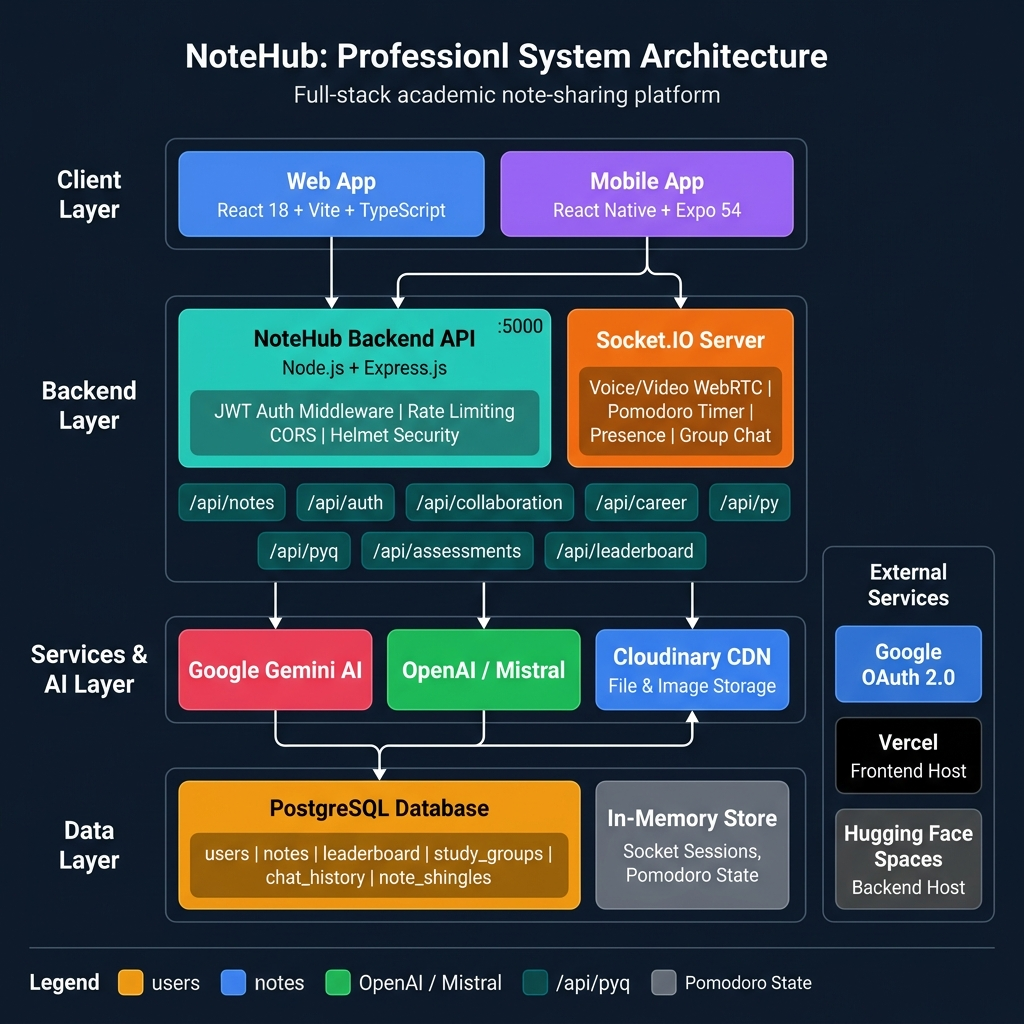
\includegraphics[width=0.9\linewidth]{notehub_system_architecture.png}
    \caption{NoteHub High-Level System Architecture}
    \label{fig:system_arch_ch3}
\end{figure}

The system architecture diagram (Figure~\ref{fig:system_arch_ch3}) outlines how the web and mobile clients connect to the Express server, which acts as the hub coordinating the PostgreSQL database, Socket.io, Gemini/Mistral APIs, and storage endpoints.

\section{FUNCTIONAL REQUIREMENTS}
Functional requirements define the specific behaviors, data processing steps, and workflows that the system must perform.

\subsection{Module F1: User Authentication and Profile Management}
\begin{itemize}
    \item \textbf{F1.1 Google OAuth 2.0 Sign-In:} The system must allow users to register and log in using Google accounts. The student initiates the login on the client device, which retrieves the Google identity token and posts it to the backend route \texttt{POST /api/auth/google}. The backend utilizes the \texttt{google-auth-library} to verify the payload signature against Google's public key sets. Upon verification, the backend queries the \texttt{users} database table. If no matching email is found, a new user record is created with a default point balance of zero and role set to "student". If registered, the system logs the entry. The server signs a JSON Web Token (JWT) containing the user ID, email, and role, using symmetric secret key \texttt{JWT\_SECRET} with a 24-hour expiration, and returns the token to the client.
    
    \textit{Input Parameters:} \texttt{\{ idToken: string \}} sent via request body. \\
    \textit{Processing Steps:} Load Google public JWKs, execute signature verification, parse payload claims (email, name, picture), select or insert record in the database, and compile signed JWT. \\
    \textit{Output Data:} \texttt{\{ token: string, user: \{ id: string, name: string, email: string, role: string \} \}} returned as JSON.
    
    \item \textbf{F1.2 Admin Whitelist Validation:} Access to the administrative web dashboard must be restricted to approved accounts. When a user attempts to log in as an administrator, the backend authentication controller validates the credentials and executes a database query matching the administrator's email against the \texttt{admin\_whitelist} table. If the email is not present on the whitelist, the backend immediately rejects the request with HTTP 403 Forbidden, preventing unauthorized administrative access and writing a security exception to logs.
    
    \textit{Input Parameters:} User email retrieved from authenticated Google claim. \\
    \textit{Processing Steps:} Query whitelisted email matching table. Reject with error code if domain or exact email is absent. \\
    \textit{Output Data:} Access status code (200 OK or 403 Forbidden).
    
    \item \textbf{F1.3 JWT Session Authorization Middleware:} To secure API endpoints, the Express server must run authorization middleware. For all protected routes, the middleware extracts the token from the \texttt{Authorization: Bearer <token>} HTTP request header. It validates the cryptographic signature using the backend's symmetric key \texttt{JWT\_SECRET}. If the signature is valid and the token has not expired, the middleware attaches the decoded payload (containing user ID and role) to the request object and invokes the next handler. Otherwise, it returns HTTP 401 Unauthorized.
    
    \textit{Input Parameters:} \texttt{Authorization} request header. \\
    \textit{Processing Steps:} Split token from header string, run \texttt{jwt.verify()}, extract signature, check expiration against server epoch. \\
    \textit{Output Data:} Request wrapper additions or HTTP 401 response.
    
    \item \textbf{F1.4 Gamified Profile Dashboard:} The backend must expose an API route \texttt{GET /api/users/profile} to retrieve user achievements. The database controller aggregates details for the logged-in student: the total number of notes uploaded, the count of completed quizzes, the cumulative point balance, and a list of badge milestones achieved (joining the \texttt{user\_badges} and \texttt{badges} tables). The server compiles these statistics into a JSON response, which is rendered on the client dashboard.
    
    \textit{Input Parameters:} User ID from active session token. \\
    \textit{Processing Steps:} Run joint SELECT queries across user statistics, badges, and point tables. \\
    \textit{Output Data:} JSON object containing points, uploads count, active badges, and rank.
\end{itemize}

\subsection{Module F2: Document Upload and Storage}
\begin{itemize}
    \item \textbf{F2.1 File Ingestion API:} The backend must expose the route \texttt{POST /api/notes/upload} to handle document files. The endpoint accepts a multipart form request containing the file stream and associated text fields. The file controller utilizes the \texttt{multer} middleware to intercept the payload, checking that the MIME type is \texttt{application/pdf} or an image format, and ensuring the binary size is below the 15MB system limit. If the file exceeds this limit or has an invalid format, the request is rejected with HTTP 400 Bad Request.
    
    \textit{Input Parameters:} Multipart form payload containing file stream and string metadata. \\
    \textit{Processing Steps:} Inspect header fields, check buffer array length, validate file extensions. \\
    \textit{Output Data:} Upload ID or HTTP 400 validation error.
    
    \item \textbf{F2.2 Asynchronous Storage Upload and Fallback:} Upon receiving a valid file, the backend controller attempts to upload the binary buffer to the Cloudinary API. The upload operation is protected by a timeout limit of 8 seconds. If Cloudinary fails to respond or returns a rate limit error, the upload service automatically catches the exception, switches the target destination to Supabase Storage, uploads the file, and retrieves the generated public access URL, logging the fallback execution for monitoring.
    
    \textit{Input Parameters:} File stream buffer. \\
    \textit{Processing Steps:} Attempt Cloudinary upload SDK. Catch timeout, invoke fallback Axios stream post to Supabase bucket. \\
    \textit{Output Data:} Remote public asset URL.
    
    \item \textbf{F2.3 Metadata Curriculum Tagging:} Users must assign categorical tags to uploaded notes. The upload request payload must include parameters for Course, Branch, Year, Semester, Subject, and Unit. The backend validates these inputs against database directories (matching the \texttt{subjects} and \texttt{courses} tables) to guarantee consistency. If valid, a new row is inserted into the \texttt{notes} table with status set to "pending", establishing a relational link to the note metadata.
    
    \textit{Input Parameters:} \texttt{\{ courseId: string, branchId: string, subjectId: string, unit: integer \}}. \\
    \textit{Processing Steps:} Query databases to check foreign key constraints, save note entity wrapper. \\
    \textit{Output Data:} Relational metadata object confirmed.
\end{itemize}

\subsection{Module F3: Multi-Layer Plagiarism and AI Verification Pipeline}
\begin{itemize}
    \item \textbf{F3.1 Lexical Winnowing Plagiarism Check:} The verification process must normalize the extracted document text by removing whitespace and punctuation, chunking it into $k$-grams ($k=20$), calculating hashes, and selecting min-hashes within a sliding window ($w=15$). These fingerprints are matched against database shingles, flagging notes with similarity score $S_{winnowing} \ge 40\%$. If similarity exceeds this threshold, the upload is rejected, and a plagiarism flag is set on the note record.
    
    \textit{Input Parameters:} Normal text string extracted from the document. \\
    \textit{Processing Steps:} Generate k-gram window hashes, run sliding min-hash selectors, perform SQL query comparison. \\
    \textit{Output Data:} Lexical match percentage report.
    
    \item \textbf{F3.2 Semantic SimHash Near-Duplicate Check:} The system must calculate a 64-bit SimHash value based on the term frequency-inverse document frequency (TF-IDF) of the note's text vocabulary. It stores the generated 64-bit integer on the note record. When a new note is processed, the database performs a bitwise XOR similarity check against all existing SimHash records. The Hamming distance is computed by counting the set bits:
    \begin{equation}
    \text{HammingDistance}(H_{new}, H_{existing}) = \text{popcount}(H_{new} \oplus H_{existing})
    \end{equation}
    If the distance is less than or equal to 3, the note is flagged as a near-duplicate, and the status is set to \texttt{"failed\_verification"}.
    
    \textit{Input Parameters:} Extracted term lists. \\
    \textit{Processing Steps:} Compute hash signatures, execute bitwise similarity evaluation. \\
    \textit{Output Data:} Hamming distance integer.
    
    \item \textbf{F3.3 Live Web Search Crawling:} The pipeline must select the top 5 sentences with the highest information density (based on length and distinct keywords) from the document text. The backend queries the Google Custom Search API with these sentence strings, extracts the text content of the top 3 matching web URLs, and computes the Jaccard similarity coefficient:
    \begin{equation}
    \text{Jaccard}(A, B) = \frac{|A \cap B|}{|A \cup B|}
    \end{equation}
    If the coefficient exceeds $0.5$, the matching URL is logged as a source of plagiarism, and the document is rejected.
    
    \textit{Input Parameters:} Sentences selection. \\
    \textit{Processing Steps:} Perform Axios GET requests, parse retrieved HTML bodies, evaluate set similarity metrics. \\
    \textit{Output Data:} Web sources Jaccard index.
    
    \item \textbf{F3.4 Gemini AI Content Audit:} The verification service sends text samples to the Gemini 2.0 Flash API with a custom system prompt. The model analyzes the text to determine if it is readable study material, identifies gibberish or corrupted scans, checks alignment with specified subject tags, and ensures it is not a syllabus copy. The API returns a structured JSON payload: \texttt{\{ "passed": boolean, "reason": string \}}. If "passed" is false, the note status in the database is set to \texttt{"failed\_verification"}.
    
    \textit{Input Parameters:} Document text sample text. \\
    \textit{Processing Steps:} Assemble API prompt instructions, verify payload outputs. \\
    \textit{Output Data:} Audit approval payload.
\end{itemize}

\subsection{Module F4: Semantic Note Search and Discovery}
\begin{itemize}
    \item \textbf{F4.1 Natural Language Search API:} The endpoint \texttt{GET /api/notes/search} handles semantic query searches. The backend receives a query string, converts it into a 1536-dimensional vector embedding using Gemini's text-embedding engine, and queries the database:
    \begin{equation}
    \mathbf{q} = \text{Embedding}(\text{query})
    \end{equation}
    The SQL query computes the cosine distance using the pgvector operator \texttt{<=>}:
    \begin{lstlisting}[language=SQL]
    SELECT id, title, description, 1 - (embedding <=> $1) AS similarity 
    FROM note_chunks 
    WHERE 1 - (embedding <=> $1) >= 0.70 
    ORDER BY similarity DESC LIMIT 10;
    \end{lstlisting}
    This returns the top 10 matching note chunks.
    
    \textit{Input Parameters:} Semantic text query parameters. \\
    \textit{Processing Steps:} Generate embedding vectors, execute pgvector database search. \\
    \textit{Output Data:} JSON array of matched notes metadata.
    
    \item \textbf{F4.2 Structured Filters:} The search API must support hard filter options. The backend appends conditional SQL clauses (such as \texttt{AND branch = $2 AND semester = $3 AND subject = $4}) to the semantic pgvector query, limiting the search scope to selected categories before calculating cosine similarity.
    
    \textit{Input Parameters:} Tag parameters. \\
    \textit{Processing Steps:} Incorporate filters into SQL query bindings. \\
    \textit{Output Data:} Filtered results JSON payload.
\end{itemize}

\subsection{Module F5: AI Career Advisor Chat (RAG)}
\begin{itemize}
    \item \textbf{F5.1 RAG Search Context Integration:} The chat endpoint \texttt{POST /api/career/chat} accepts the student's question. The backend generates an embedding of the query, searches the \texttt{note\_chunks} table using pgvector cosine similarity, and retrieves the top 5 most relevant text chunks. These chunks are formatted into a context block and injected into the Gemini 2.0 Flash prompt. This ensures the advisor's answers align with the student's actual syllabus materials.
    
    \textit{Input Parameters:} Question query string. \\
    \textit{Processing Steps:} Fetch embeddings, execute pgvector query, construct prompt context block, stream model output. \\
    \textit{Output Data:} Streamed advisor response text.
    
    \item \textbf{F5.2 Interactive Chat UI:} The client application must render the career advisor interface, supporting typing indicators, message bubbles, markdown rendering for structured career roadmaps, and buttons to save the roadmap to local storage.
    
    \textit{Input Parameters:} Client message logs. \\
    \textit{Processing Steps:} Bind layout components, update screen states, execute text copying. \\
    \textit{Output Data:} Visual display render states.
    
    \item \textbf{F5.3 Persistent Chat History:} The system must save chat logs in the database. Each chat message is stored in the \texttt{chat\_messages} table, linked to a session ID. When a student reopens the career advisor screen, the app calls \texttt{GET /api/career/history} to load the message history.
    
    \textit{Input Parameters:} Session ID parameter. \\
    \textit{Processing Steps:} Load chat rows, format entries, dispatch arrays to client. \\
    \textit{Output Data:} Historical messages logs database array.
\end{itemize}

\subsection{Module F6: SnapSolve OCR Solver}
\begin{itemize}
    \item \textbf{F6.1 Image Capture and Upload:} The mobile client integrates the device camera using \texttt{expo-image-picker}. The app allows the student to capture an image of a math problem or text block, crop the target area, convert the selection to a base64 buffer, and post it to \texttt{POST /api/solver/solve}.
    
    \textit{Input Parameters:} Base64 image payload wrapper. \\
    \textit{Processing Steps:} Validate image parameters, compile buffer arrays. \\
    \textit{Output Data:} Uploaded image data details.
    
    \item \textbf{F6.2 Gemini Vision Solver:} The backend uploads the image buffer to Gemini's vision endpoint. Gemini parses the math formulas, runs OCR to extract the question text, and returns a step-by-step solution formatted in LaTeX.
    
    \textit{Input Parameters:} Image data stream. \\
    \textit{Processing Steps:} Dispatch multimodal prompt, execute vision calculations. \\
    \textit{Output Data:} Step-by-step explanation LaTeX output.
\end{itemize}

\subsection{Module F7: Assessment AI Quiz Generator}
\begin{itemize}
    \item \textbf{F7.1 Automatic MCQ Generation:} The endpoint \texttt{POST /api/quiz/generate} parses the note's text, extracts key technical concepts, and calls the Gemini API to construct a 5-question multiple-choice quiz with four options per question and a verified answer key, returning it as structured JSON.
    
    \textit{Input Parameters:} Note ID. \\
    \textit{Processing Steps:} Fetch text, format template requirements, parse output JSON structures. \\
    \textit{Output Data:} 5 MCQs array JSON.
    
    \item \textbf{F7.2 Real-time Quiz Grading:} The client app must validate user answers, calculate the score, and post results to \texttt{POST /api/quiz/submit}. If the score is $\ge 80\%$, the server awards 10 contribution points and updates the database records.
    
    \textit{Input Parameters:} Quiz ID, user selected answers array. \\
    \textit{Processing Steps:} Verify options, compute score percentage, execute score award database updates. \\
    \textit{Output Data:} Score card JSON report.
\end{itemize}

\subsection{Module F8: Collaborative Study Rooms}
\begin{itemize}
    \item \textbf{F8.1 Socket Room Joins:} The Socket.io connection controller must listen for \texttt{join\_room} events. It validates the user's authorization token, registers their socket ID to the room channel, and broadcasts a join notification.
    
    \textit{Input Parameters:} Socket packet data. \\
    \textit{Processing Steps:} Verify token signature, subscribe client socket to targeted channel. \\
    \textit{Output Data:} Socket channel confirmation.
    
    \item \textbf{F8.2 Real-time Messages Broadcast:} The server must broadcast \texttt{send\_message} events. It receives the message payload, persists it to the database table \texttt{messages}, and broadcasts it to all active sockets in the room channel in under 150ms.
    
    \textit{Input Parameters:} Message text and room reference. \\
    \textit{Processing Steps:} Store message entry in SQL, broadcast package payload to room channel. \\
    \textit{Output Data:} Broadcasted packet message event.
    
    \item \textbf{F8.3 Peer Help Request Board:} Students can dispatch a \texttt{help\_request} event, which publishes a question banner on the study room's board. Online classmates can click "Accept" to join their chat, earning 20 contribution points when marked as resolved.
    
    \textit{Input Parameters:} Help request parameters. \\
    \textit{Processing Steps:} Update board listing status, emit socket updates. \\
    \textit{Output Data:} Board additions event dispatch.
    
    \item \textbf{F8.4 Sockets Profanity Filter Middleware:} The server socket middleware must pass incoming chat text strings to the \texttt{leo-profanity} utility library. If any profane words match, they are replaced with asterisks before being broadcasted.
    
    \textit{Input Parameters:} Raw chat text string. \\
    \textit{Processing Steps:} Parse string characters, match against blocked list dictionary, execute asterisk substitution. \\
    \textit{Output Data:} Cleaned chat string output.
\end{itemize}

\subsection{Module F9: Gamification and Leaderboards}
\begin{itemize}
    \item \textbf{F9.1 Automated Points Awarding:} The backend must execute transactions to increment student points. Point values are defined as: 50 points for verified note uploads, 20 points for resolving peer help requests, and 10 points for scoring over 80\% on quizzes.
    
    \textit{Input Parameters:} User reference, points increment type indicator. \\
    \textit{Processing Steps:} Execute SQL TRANSACTION updates, prevent concurrent lock collisions. \\
    \textit{Output Data:} Confirmed points updates.
    
    \item \textbf{F9.2 Badge Milestones:} When a user's point total exceeds thresholds (e.g., 500, 1000, 2500 points), the backend awards badges and updates the profile, triggering a socket banner notification to the student.
    
    \textit{Input Parameters:} User point totals. \\
    \textit{Processing Steps:} Check thresholds metrics, insert badge references. \\
    \textit{Output Data:} Unlocked badges notification alert.
    
    \item \textbf{F9.3 Real-Time Global Leaderboard:} The database view \texttt{leaderboard\_view} must sort active users in descending order of points, exposing a fast cached API endpoint to display user ranks and profile links.
    
    \textit{Input Parameters:} None (public API call). \\
    \textit{Processing Steps:} Retrieve sorted database profiles. \\
    \textit{Output Data:} Leaderboard profiles JSON arrays.
\end{itemize}

\section{NON-FUNCTIONAL REQUIREMENTS}
Non-functional requirements specify the performance, security, and quality constraints of the platform.

\subsection{Performance Specifications}
\begin{itemize}
    \item \textbf{Sub-Second Vector Search:} Similarity queries using the pgvector extension must return the top 5 nearest neighbors in under 200 milliseconds.
    \item \textbf{Low-Latency APIs:} Standard REST API endpoints (excluding document verification and AI calls) must return JSON responses in under 250 milliseconds under normal network conditions.
    \item \textbf{Fast Initial Render:} The web application's initial DOM rendering must complete in under 1.5 seconds, utilizing code splitting to load components only as needed.
    \item \textbf{Real-time WebSocket Broadcasts:} Socket.io messages must be delivered to all users in a room with a latency under 150 milliseconds.
\end{itemize}

\subsection{Reliability and Fault Tolerance}
\begin{itemize}
    \item \textbf{Dual Storage Fallback:} If Cloudinary experiences a timeout or rate limit error, the file upload route must automatically fall back to Supabase Storage, preventing upload failures.
    \item \textbf{AI API Failover:} If the primary Gemini API endpoint is unavailable, the backend must redirect requests to the fallback Mistral API or a local Ollama service.
    \item \textbf{Connection Pooling:} The backend must use connection pooling (via \texttt{pg.Pool}) to manage database connections, automatically reconnecting if the database server restarts.
    \item \textbf{Socket Auto-Reconnect:} The mobile and web clients must be configured to automatically attempt reconnection if the WebSocket link drops.
\end{itemize}

\subsection{Security and Data Integrity}
\begin{itemize}
    \item \textbf{Helmet HTTP Headers:} The Express backend must use the Helmet middleware to set security headers, protecting the system against clickjacking, cross-site scripting (XSS), and MIME sniffing.
    \item \textbf{JWT Token Verification:} All routes except authentication and public notes search must require a valid JWT token in the Authorization header. The token must expire in 24 hours.
    \item \textbf{Input Sanitization:} To prevent SQL injection and XSS attacks, all inputs must be sanitized using parameterized queries in PostgreSQL.
    \item \textbf{Bcrypt Hashing:} Passwords for custom student logins must be hashed with a salt round of 10 using bcrypt before storage.
\end{itemize}

\subsection{Usability and Interface Standards}
\begin{itemize}
    \item \textbf{Standardized Light Theme:} NoteHub implements a standardized light theme ("NoteHub Light") to ensure a consistent, clean, and professional interface.
    \item \textbf{Responsive Grid Layouts:} The web application must adapt to varying viewport widths (desktop, tablet, mobile) using CSS Grid and Flexbox.
    \item \textbf{Custom Sockets Navigation:} The mobile client must implement an animated custom navigation bar to switch between Notes, Collaborate, Snap AI, and Career Advisor screens.
    \item \textbf{Accessibility Compliance:} The user interface must align with WCAG 2.1 Level AA requirements. All text elements must maintain contrast ratios above 4.5:1. Mobile elements must be touch-target optimized with minimum dimension profiles of 44x44 points.
\end{itemize}

\subsection{Scalability Boundaries}
\begin{itemize}
    \item \textbf{Docker Containerization:} The backend services must be packaged in Docker containers to ensure identical configurations across development, testing, and production.
    \item \textbf{Asynchronous Worker Processes:} The document verification pipeline must process files asynchronously, freeing backend thread resources to handle other incoming API requests.
    \item \textbf{Horizontal Scalability:} The API server is modeled to support horizontal scalability. Using a stateless session paradigm (JWT validation and PostgreSQL state management), multiple backend container instances can be run behind an Nginx load balancer to support larger traffic loads.
\end{itemize}

\section{PERFORMANCE REQUIREMENTS}
Performance requirements define the numerical metrics the system must satisfy.

\begin{table}[htbp]
\centering
\caption{NoteHub Target Performance Metrics}
\label{tab:perf_metrics}
\resizebox{\textwidth}{!}{%
\begin{tabular}{|l|p{6cm}|p{6.5cm}|}
\hline
\textbf{Parameter ID} & \textbf{Metric Description} & \textbf{Target Value / Threshold} \\
\hline
PERF-01 & End-to-end PDF processing latency & $< 60$ seconds (including OCR and AI checks) \\
\hline
PERF-02 & pgvector query execution time & $< 200$ milliseconds under $N \le 10,000$ rows \\
\hline
PERF-03 & Socket.io broadcast latency & $< 150$ milliseconds (client-to-client loop) \\
\hline
PERF-04 & Standard REST JSON response time & $< 250$ milliseconds under normal network load \\
\hline
PERF-05 & Plagiarism model precision and recall & Precision $ge 92\%$, Recall $ge 95\%$ \\
\hline
PERF-06 & SnapSolve Image OCR text extraction accuracy & $ge 92\%$ under standard library light settings \\
\hline
PERF-07 & App memory consumption on mobile devices & $< 150$ MB RAM under note reading workflows \\
\hline
PERF-08 & Database connection pool acquisition delay & $< 20$ milliseconds under peak usage thresholds \\
\hline
\end{tabular}%
}
\end{table}

The numerical constraints defined in Table~\ref{tab:perf_metrics} act as the performance boundary. Failing to stay within these limits triggers automatic system alerts on the server dashboards.

\section{DESIGN CONSTRAINTS}
Design constraints represent the technological limitations, policies, and environment restrictions of the project.

\subsection{Mobile Framework Restrictions}
NoteHub uses React Native with the Expo SDK. This restricts the mobile client to Expo-supported libraries and native modules. Any custom native Android or iOS libraries must be compatible with Expo's configuration system, preventing direct installation of unverified native packages. PDF rendering on the mobile client is constrained to webview integrations or basic document readers.

\subsection{Database Indexing Restrictions}
PostgreSQL with pgvector supports IVFFlat and HNSW indexes. While HNSW offers high recall and search speeds, it requires significant server memory. NoteHub is deployed on Render's free tier, which restricts memory to 512MB. This memory limit prevents the use of large HNSW indexes, requiring the database to fall back to optimized B-Tree and IVFFlat indexes to avoid memory issues.

\subsection{API Rate Limits and Quotas}
NoteHub relies on free-tier APIs for generative AI and search crawling:
\begin{itemize}
    \item \textbf{Google Gemini 2.0 Flash API:} Restricts requests to 15 RPM (requests per minute) and 1,000 RPD (requests per day).
    \item \textbf{Google Custom Search API:} Restricts free search queries to 100 queries per day.
\end{itemize}
To operate within these quotas, NoteHub must implement local caching of search results and limit AI calls per user to 5 requests per minute.

\subsection{Platform Regulatory and Security Compliance}
NoteHub must respect data privacy guidelines. All user data, especially emails collected via Google OAuth 2.0, must be encrypted in transit using TLS 1.3 and stored with encryption-at-rest. Chat message databases are periodically pruned of expired study room sessions, and students can request account deletions, which triggers cascade deletes across users, notes, points, and chat indexes.

\section{SYSTEM REQUIREMENTS}
This section outlines the hardware and software specifications for the development and deployment of NoteHub.

\subsection{Hardware Requirements}
Table~\ref{tab:hardware_specs} lists the hardware specifications for the development server and client devices.

\begin{table}[htbp]
\centering
\caption{System Hardware Specifications}
\label{tab:hardware_specs}
\resizebox{\textwidth}{!}{%
\begin{tabular}{|l|p{7cm}|p{7cm}|}
\hline
\textbf{Component} & \textbf{Development/Server Specifications} & \textbf{Client Device Specifications} \\
\hline
Processor          & Intel Core i5 / AMD Ryzen 5 (2.5 GHz quad-core) or above. & Quad-core processor (ARM-based for mobile, x86/ARM for web client). \\
\hline
RAM                & 8 GB DDR4 (16 GB recommended for running Docker and DB locally). & 4 GB RAM (mobile devices), 4 GB RAM (desktop web clients). \\
\hline
Storage            & 256 GB SSD (with 20 GB free space for database caching). & 500 MB free space (for caching PDFs and assets on mobile client). \\
\hline
Network            & High-speed broadband connection (minimum 10 Mbps). & Active internet connection (4G/5G mobile data or Wi-Fi). \\
\hline
Display            & 1080p monitor for development. & Minimum display resolution of 720x1280 (mobile), 1024x768 (desktop). \\
\hline
\end{tabular}%
}
\end{table}

\subsection{Software Requirements}
Table~\ref{tab:software_specs} lists the software packages, frameworks, and tools used in NoteHub.

\begin{table}[htbp]
\centering
\caption{System Software Specifications}
\label{tab:software_specs}
\resizebox{\textwidth}{!}{%
\begin{tabular}{|l|l|l|p{5.5cm}|}
\hline
\textbf{Software Type} & \textbf{Technology / Library} & \textbf{Version} & \textbf{Purpose} \\
\hline
Runtime Environment & Node.js & v20.x LTS & JavaScript runtime for backend services. \\
\hline
Backend Framework   & Express.js & v4.19.x & REST API framework for routing. \\
\hline
Database Engine     & PostgreSQL & v15.x & Persistent relational and vector storage. \\
\hline
Vector Search       & pgvector & v0.5.x & High-dimensional embedding storage/search. \\
\hline
Real-Time Sync      & Socket.io & v4.7.x & WebSocket connection management. \\
\hline
Frontend Framework  & React.js & v18.x & Web user interface development. \\
\hline
Web Bundler         & Vite & v5.x & Fast web client builds and hot reloading. \\
\hline
Mobile Framework    & React Native / Expo & SDK 54 & Cross-platform native mobile development. \\
\hline
Security Middleware & Helmet & v7.x & HTTP security headers configuration. \\
\hline
Cryptography        & bcrypt & v5.x & Hashing password credentials. \\
\hline
\end{tabular}%
}
\end{table}

This software configuration guarantees environment consistency and ensures that NoteHub compiles and runs reliably on cloud platforms.
\chapter{SYSTEM PLANNING}
\rule{\textwidth}{1pt}

\section{INTRODUCTION}
Software project planning is the foundation of successful software engineering. It involves coordinating human resources, scheduling development phases, assessing technical risks, and establishing quality standards to deliver a product on time and within budget. For NoteHub, proper planning is especially critical due to the complex integration of cross-platform frontend interfaces (React.js web and React Native mobile), real-time WebSocket communication, and generative AI services (Google Gemini 2.0 Flash). 

The strategy for NoteHub was built around three planning principles:
\begin{itemize}
    \item \textbf{Incremental Integration:} Rather than building all components in isolation and attempting a single "big bang" integration, the system was planned to build and test features incrementally. Each core backend route and corresponding database table was verified before developing frontend clients.
    \item \textbf{Continuous Risk Mitigation:} Technical risks, such as generative AI API rate limits and vector database query latencies, were identified early. The project schedule included dedicated slots to build fallback mechanisms and query optimizations.
    \item \textbf{Rigor in Quality Assurance:} Testing was integrated into the development cycle. Sprints included time to write unit tests for the plagiarism and vector pipelines, ensuring that issues were caught and debugged early.
\end{itemize}

By establishing a structured software development life cycle (SDLC) model, defining a detailed timeline, and outlining monitoring and control procedures, the development team ensured that NoteHub was developed, tested, and deployed within a single academic semester.

\section{SDLC MODEL}
To manage the complexity of NoteHub, the team adopted the \textbf{Agile Scrum} Software Development Life Cycle (SDLC) model. 

\subsection{Why Agile Scrum was Chosen Over Waterfall}
Traditional software development models, such as the Waterfall model, operate sequentially. Each phase (requirements, design, implementation, verification, and maintenance) must be completed before the next begins. While Waterfall works well for systems with static requirements, it is poorly suited for modern AI-integrated applications. 

NoteHub relied on third-party generative AI and web crawling APIs. During development, these external APIs frequently updated their endpoints, rate limits, and pricing structures. A sequential Waterfall model would be too rigid to accommodate these changes. If the API rate limits shifted during the implementation phase, modifying the system architecture would require repeating requirements and design phases, causing major delays.

Agile Scrum resolves these issues by breaking development into short, iterative cycles called \textbf{sprints}. This iterative approach provided several advantages for NoteHub:
\begin{itemize}
    \item \textbf{Flexibility:} If a rate limit threshold changed or an external API went offline, the team adapted the architecture in the next sprint (e.g., implementing the Supabase storage fallback and local caching).
    \item \textbf{Incremental Testing:} Each sprint produced a working component that was immediately tested. This allowed the team to find performance bottlenecks in the plagiarism checker and vector database queries early, rather than waiting until the end of the project.
    \item \textbf{Improved Collaboration:} Daily stand-ups and sprint retrospectives kept team members aligned, helping coordinate frontend web and mobile development with the backend API.
\end{itemize}

\subsection{Agile Scrum Phases and Activities}
The development of NoteHub followed standard Scrum practices, utilizing 2-week sprints. Each sprint followed a rigid sequence of agile ceremonies:
\begin{enumerate}
    \item \textbf{Product Backlog Grooming:} The team compiled all features (authentication, upload, plagiarism checks, career advisor, leaderboard) into a prioritized list of user stories.
    \item \textbf{Sprint Planning:} At the beginning of each sprint, the team selected high-priority user stories, estimated their complexity using story points, and committed to a sprint backlog.
    \item \textbf{Daily Stand-ups:} The team held 15-minute daily meetings to discuss progress, plan daily tasks, and identify blockers.
    \item \textbf{Sprint Reviews:} At the end of each sprint, the team demonstrated working features (e.g., a functioning Socket.io study room or a successful pgvector query) to obtain feedback.
    \item \textbf{Sprint Retrospectives:} The team reflected on the sprint process, identifying improvements to make the next sprint more efficient.
\end{enumerate}

\subsection{Detailed Sprint Narrative and User Stories}
The 14-week project timeline was divided into 7 distinct development sprints:
\begin{itemize}
    \item \textbf{Sprint 1 (Weeks 1--2) --- Requirement Analysis and Schema Setup:} Focus on requirement elicitation, system overview design, and database planning. The team drafted the database schema, including notes, users, and messaging tables, and configured a local PostgreSQL server with the pgvector extension.
    \begin{itemize}
        \item \textit{User Story US1.1:} As a developer, I want to establish a database schema with relational and vector capabilities so that student records and high-dimensional document chunks can be stored in the same database.
        \item \textit{Acceptance Criteria:} PostgreSQL database must initialize successfully; pgvector extension must compile and execute test cosine similarity queries.
        \item \textit{Story Points:} 5 SP.
        \item \textit{Sprint Review Outcome:} Initial relational tables mapped; pgvector test queries returned results in under 5ms.
    \end{itemize}
    \begin{itemize}
        \item \textit{User Story US1.2:} As a system analyst, I want to document the functional specifications so that the developers have a clear understanding of the project modules.
        \item \textit{Acceptance Criteria:} System specs document created; verified and signed off by the project guide.
        \item \textit{Story Points:} 3 SP.
        \item \textit{Sprint Review Outcome:} System Analysis and Specifications document finalized.
    \end{itemize}
    
    \item \textbf{Sprint 2 (Weeks 3--4) --- Core Backend Setup and Auth:} Set up the Node.js/Express.js backend structure. Developed user authentication APIs, integrated Google OAuth 2.0, and implemented JWT token creation. Set up the admin whitelist portal, restricting administrative dashboard access.
    \begin{itemize}
        \item \textit{User Story US2.1:} As a student, I want to log in using my Google account so that I can access my notes and study rooms securely without creating a new password.
        \item \textit{Acceptance Criteria:} Token validation must be processed on the backend using the \texttt{google-auth-library}; successful verification must return a signed JWT token.
        \item \textit{Story Points:} 5 SP.
        \item \textit{Sprint Review Outcome:} Authentication middleware verified; whitelisted admin accounts successfully bypassed standard student routing.
    \end{itemize}
    \begin{itemize}
        \item \textit{User Story US2.2:} As an administrator, I want to view a whitelist portal so that only approved accounts can access the admin dashboard.
        \item \textit{Acceptance Criteria:} Whitelist validation query on database; API blocks unauthorized administrative logins.
        \item \textit{Story Points:} 3 SP.
        \item \textit{Sprint Review Outcome:} Admin portal whitelist interface established and tested with invalid credentials.
    \end{itemize}
    
    \item \textbf{Sprint 3 (Weeks 5--6) --- Document Ingestion Pipeline:} Built document upload APIs, integrating text extraction and storage. Configured the Express backend to upload files to Cloudinary, and developed the Supabase Storage fallback mechanism to handle Cloudinary failures.
    \begin{itemize}
        \item \textit{User Story US3.1:} As a student, I want to upload a PDF note and have the system save it securely so that other students can discover it.
        \item \textit{Acceptance Criteria:} The uploader must accept PDF files under 15MB; it must upload them to Cloudinary and fall back to Supabase Storage if Cloudinary is offline.
        \item \textit{Story Points:} 8 SP.
        \item \textit{Sprint Review Outcome:} File upload pipeline integrated; fallback trigger successfully redirected uploads to Supabase during simulated Cloudinary timeouts.
    \end{itemize}
    \begin{itemize}
        \item \textit{User Story US3.2:} As a system components integrator, I want to parse uploaded PDF documents and extract raw text on the server.
        \item \textit{Acceptance Criteria:} Use \texttt{pdf-parse} to extract text, validate that non-empty text strings are returned, and return a clean JSON payload.
        \item \textit{Story Points:} 5 SP.
        \item \textit{Sprint Review Outcome:} PDF parsing verified with multi-column text formats and diagrams.
    \end{itemize}
    
    \item \textbf{Sprint 4 (Weeks 7--8) --- Plagiarism Algorithms:} Implemented core plagiarism detection check. Coded the Winnowing fingerprinting algorithm and the 64-bit SimHash near-duplicate check. Developed the sentence-level web crawler to scrape search engines for online plagiarized matches.
    \begin{itemize}
        \item \textit{User Story US4.1:} As an administrator, I want the system to check uploaded notes for plagiarism so that duplicate or copy-pasted content is flagged automatically.
        \item \textit{Acceptance Criteria:} Winnowing algorithm must extract k-grams and select min-hashes; SimHash must calculate bitwise distance; copied files must be flagged.
        \item \textit{Story Points:} 8 SP.
        \item \textit{Sprint Review Outcome:} Plagiarism utility modules verified; near-duplicate notes were detected and flagged within a 25-second processing window.
    \end{itemize}
    \begin{itemize}
        \item \textit{User Story US4.2:} As a student, I want the system to search the public web for plagiarized text in my notes so that I know if my content matches online sources.
        \item \textit{Acceptance Criteria:} Parse document into sentences, query search engine API, analyze and aggregate similarity scores.
        \item \textit{Story Points:} 8 SP.
        \item \textit{Sprint Review Outcome:} Web crawler script completed and integrated with custom search engines, returning exact URL matches.
    \end{itemize}
    
    \item \textbf{Sprint 5 (Weeks 9--10) --- AI Integration and RAG:} Integrated Google Gemini 2.0 Flash APIs. Set up document text chunking and embedding generation, storing vectors in pgvector. Developed the RAG pipeline to retrieve relevant notes context for the AI Career Advisor. Coded SnapSolve and Assessment AI.
    \begin{itemize}
        \item \textit{User Story US5.1:} As a student, I want to ask career questions and receive advice based on my study notes so that I can prepare for my future role.
        \item \textit{Acceptance Criteria:} The RAG query must run a cosine similarity search on pgvector; retrieved context must be sent to Gemini to generate the response.
        \item \textit{Story Points:} 8 SP.
        \item \textit{Sprint Review Outcome:} RAG career chat operational; response generation times averaged 2.8 seconds, returning syllabus-aligned roadmaps.
    \end{itemize}
    \begin{itemize}
        \item \textit{User Story US5.2:} As a student, I want to capture a picture of a question and get a step-by-step solution immediately.
        \item \textit{Acceptance Criteria:} Send image buffer to Gemini 2.0 Flash vision endpoints; parse the returned explanation payload; render on the mobile client.
        \item \textit{Story Points:} 8 SP.
        \item \textit{Sprint Review Outcome:} SnapSolve visual solver implemented; OCR and math formula rendering validated on mobile screens.
    \end{itemize}
    
    \item \textbf{Sprint 6 (Weeks 11--12) --- Sockets and Collaboration:} Developed real-time features using Socket.io 4. Configured namespace rooms for study groups, coded the live peer help board, and integrated chat profanity filters.
    \begin{itemize}
        \item \textit{User Story US6.1:} As a student, I want to join a study room and chat in real-time with my classmates so that we can collaborate on notes.
        \item \textit{Acceptance Criteria:} Socket.io must establish namespace channels; messages must broadcast instantly; profane words must be filtered.
        \item \textit{Story Points:} 5 SP.
        \item \textit{Sprint Review Outcome:} WebSocket channels verified; chat messages broadcasted in under 100ms; \texttt{leo-profanity} replaced flagged words with asterisks.
    \end{itemize}
    \begin{itemize}
        \item \textit{User Story US6.2:} As a student in need of help, I want to post on the live peer help board so that online classmates can join my room.
        \item \textit{Acceptance Criteria:} Dispatch global event when help request is posted; real-time notifications sent to active socket clients.
        \item \textit{Story Points:} 5 SP.
        \item \textit{Sprint Review Outcome:} Live help board system synchronized and real-time banner notifications working on both web and mobile.
    \end{itemize}
    
    \item \textbf{Sprint 7 (Weeks 13--14) --- Testing and Deployment:} Conducted unit, integration, and system testing. Configured Docker containers for the backend, deployed frontend clients on Vercel, and deployed backend APIs on Render.
    \begin{itemize}
        \item \textit{User Story US7.1:} As a developer, I want to containerize the backend services so that the system runs identically in development and production environments.
        \item \textit{Acceptance Criteria:} Dockerfile must build the backend image successfully; Vercel and Render deployments must connect to the live PostgreSQL database.
        \item \textit{Story Points:} 5 SP.
        \item \textit{Sprint Review Outcome:} System successfully deployed; REST APIs and Socket.io endpoints verified on production servers.
    \end{itemize}
    \begin{itemize}
        \item \textit{User Story US7.2:} As a QA engineer, I want to test the entire system for regression issues and load spikes before release.
        \item \textit{Acceptance Criteria:} Run full regression suite; simulate up to 100 concurrent socket connections; ensure database connection pooling works.
        \item \textit{Story Points:} 5 SP.
        \item \textit{Sprint Review Outcome:} System verification and load tests executed successfully; database connection limits stabilized using pool tuning.
    \end{itemize}
\end{itemize}

\section{TIMELINE AND MILESTONES}
The project schedule was planned to complete all phases within a 14-week academic semester. Table~\ref{tab:milestones_ch4} summarizes the major milestones and deliverables of the project.

\begin{table}[htbp]
\centering
\caption{Project Milestones and Deliverables}
\label{tab:milestones_ch4}
\resizebox{\textwidth}{!}{%
\begin{tabular}{|p{3cm}|p{3.5cm}|p{7.5cm}|}
\hline
\textbf{Milestone} & \textbf{Target Week} & \textbf{Expected Deliverable} \\
\hline
M1: Requirements & Week 2 & Complete System Specification Document and normalized DB schema. \\
\hline
M2: Backend Auth & Week 4 & Express.js REST API with working Google OAuth and JWT sessions. \\
\hline
M3: Ingestion    & Week 6 & File upload pipeline with Cloudinary/Supabase fallback storage. \\
\hline
M4: Plagiarism   & Week 8 & Document similarity checking running Winnowing and SimHash checks. \\
\hline
M5: AI \& RAG    & Week 10 & pgvector storage indexing and Gemini-pro Career Advisor chat. \\
\hline
M6: Sockets      & Week 12 & WebSocket chat rooms with profanity filtering and help boards. \\
\hline
M7: Deployment   & Week 14 & Docker containers deployed on Vercel and Render with Swagger docs. \\
\hline
\end{tabular}%
}
\end{table}

\subsection{Detailed Work Breakdown Structure}
To ensure all tasks were executed systematically, the team structured a detailed Work Breakdown Structure (WBS) mapping dependencies, durations, assignees, and technical deliverables. Table~\ref{tab:wbs} lists the complete breakdown of the project.

\begin{table}[htbp]
\centering
\caption{Project Work Breakdown Structure (WBS)}
\label{tab:wbs}
\resizebox{\textwidth}{!}{%
\begin{tabular}{|c|l|c|c|l|p{4.5cm}|}
\hline
\textbf{WBS ID} & \textbf{Task Name} & \textbf{Start} & \textbf{End} & \textbf{Assignee} & \textbf{Deliverable} \\
\hline
1.1 & Requirement Gathering \& Specs & W1 & W2 & Analyst & Complete System Specifications Document. \\
\hline
1.2 & Database Schema Design \& Setup & W2 & W2 & DB Eng. & normalized SQL schema with pgvector. \\
\hline
2.1 & Node.js/Express API foundation & W3 & W3 & Backend Dev. & Express boilerplate with standard structure. \\
\hline
2.2 & Google OAuth \& JWT Token Auth & W4 & W4 & Security Eng. & Secure passport token validation routes. \\
\hline
2.3 & Admin Whitelist Portal Middleware & W4 & W4 & Backend Dev. & Route protection based on whitelist table. \\
\hline
3.1 & Ingestion PDF Parser Controller & W5 & W5 & Backend Dev. & File upload endpoint with PDF text extractor. \\
\hline
3.2 & Cloudinary \& Supabase Storage API & W6 & W6 & Cloud Eng. & Fallback storage logic inside file controller. \\
\hline
4.1 & Winnowing Fingerprinting Utility & W7 & W7 & Algorithm Dev. & K-gram hashing and sliding window selector. \\
\hline
4.2 & SimHash Duplicate checker Utility & W8 & W8 & Algorithm Dev. & Bitwise frequency hashing and Hamming distance. \\
\hline
4.3 & Sentence Web Search Crawler API & W8 & W8 & Backend Dev. & Google Custom Search crawler integration. \\
\hline
5.1 & Vector Embeddings Generator & W9 & W9 & AI Eng. & text chunking and embedding logic. \\
\hline
5.2 & Gemini-pro Advisor \& pgvector RAG & W9 & W10 & AI Eng. & Similarity matches controller using Gemini. \\
\hline
5.3 & SnapSolve camera OCR \& quiz AI & W10 & W10 & Mobile Dev. & OCR solver and MCQ generator modules. \\
\hline
6.1 & Socket.io 4 connection structure & W11 & W11 & Network Eng. & Event-driven socket namespaces. \\
\hline
6.2 & Messaging Rooms \& Help board & W12 & W12 & Frontend Dev. & Collaboration chat screens with board triggers. \\
\hline
6.3 & Profanity Replacement Filters & W12 & W12 & Backend Dev. & Sockets middleware filtering using \texttt{leo-profanity}. \\
\hline
7.1 & Docker container config & W13 & W13 & DevOps Eng. & Multi-stage Dockerfiles. \\
\hline
7.2 & Testing, Debug \& Cloud Deploy & W13 & W14 & QA Eng. & System verification and production deployment. \\
\hline
\end{tabular}%
}
\end{table}

To visualize the project timeline and the overlap between sprints, a Gantt chart was constructed. 

\begin{figure}[H]
\centering
\begin{ganttchart}[
    vgrid={*2{dotted}, *1{black}},
    hgrid,
    x unit=0.7cm,
    y unit chart=0.7cm,
    time slot format=simple,
    title height=1,
    bar/.style={fill=blue!30, draw=blue!70, line width=1pt},
    bar height=0.6,
    group right shift=0,
    group top shift=0.1,
    group height=0.3
]{1}{14}
    \gantttitle{Project Development Timeline (Weeks)}{14} \\
    \gantttitlelist{1,...,14}{1} \\
    \ganttbar{Planning \& DB Schema}{1}{2} \\
    \ganttbar{Backend Auth \& API}{3}{4} \\
    \ganttbar{Ingestion \& Storage}{5}{6} \\
    \ganttbar{Plagiarism Checking}{7}{8} \\
    \ganttbar{AI \& RAG Integration}{9}{10} \\
    \ganttbar{Real-Time Sockets}{11}{12} \\
    \ganttbar{Testing \& Cloud Deploy}{13}{14}
\end{ganttchart}
\caption{Project Gantt Chart Timeline}
\label{fig:gantt_chart}
\end{figure}

Figure~\ref{fig:gantt_chart} illustrates the 14-week timeline, detailing the sequential flow of backend development and the integration of real-time communication and AI services in later weeks.

\section{RISK ANALYSIS AND MITIGATION}
Identifying and mitigating risks early was critical to avoiding project delays. We categorized risks into technical, operational, and schedule-related challenges. Table~\ref{tab:risk_matrix} maps each risk to its category, probability, impact, and mitigation strategy.

\begin{table}[htbp]
\centering
\caption{Project Risk Matrix}
\label{tab:risk_matrix}
\resizebox{\textwidth}{!}{%
\begin{tabular}{|c|p{4.5cm}|c|c|c|p{6.5cm}|}
\hline
\textbf{Risk ID} & \textbf{Risk Description} & \textbf{Likelihood} & \textbf{Impact} & \textbf{Risk Score} & \textbf{Mitigation Strategy} \\
\hline
R1 & AI API Rate Limits \& Exhaustion & 4 & 5 & 20 & Implement local caching for search results and developer-grade fallbacks (Gemini to Mistral/Ollama). \\
\hline
R2 & High Document Ingestion Latency & 3 & 3 & 9 & Process document verification asynchronously, displaying a processing status to the user. \\
\hline
R3 & Vector Database Memory Limits  & 3 & 4 & 12 & Optimize database indexes, falling back to IVFFlat or standard indexes to respect Render RAM limits. \\
\hline
R4 & WebSocket Sockets Event Drop    & 2 & 3 & 6 & Implement heartbeat intervals and client-side auto-reconnection logic. \\
\hline
R5 & Plagiarism Checks False Positives & 3 & 4 & 12 & Fine-tune Winnowing window sizes ($w$) and combine it with semantic SimHash checks. \\
\hline
R6 & Cloud Container Deploy Crashes  & 2 & 4 & 8 & Package services in Docker containers to match development and production environments. \\
\hline
R7 & Client Storage Limits on Mobile & 4 & 3 & 12 & Implement local cache cleanups and limits on cached PDF files on mobile. \\
\hline
R8 & Sockets Room Info Leakage       & 2 & 5 & 10 & Enforce strict token checks on room connections and isolate socket namespaces. \\
\hline
R9 & Supabase API Retrieval Timeouts & 2 & 4 & 8 & Implement automatic connection retries and dual storage status checks. \\
\hline
R10 & Web Crawler Rate Limiting      & 3 & 3 & 9 & Implement proxy rotation, custom API limits, and fallback internal search indexes. \\
\hline
R11 & Leaderboard Sync Race Conditions & 2 & 4 & 8 & Use transaction levels (Serializable) in PostgreSQL for leaderboard point updates. \\
\hline
R12 & JWT Expiration in Active Sockets & 2 & 3 & 6 & Implement socket refresh tokens and client hooks to validate token lifespan. \\
\hline
\end{tabular}%
}
\end{table}

\subsection{Detailed Risk Analysis and Mitigation}
\begin{itemize}
    \item \textbf{AI API Rate Limits (R1):} NoteHub's free tier is subject to strict rate limits. To prevent API exhaustion, the system caches vector embeddings locally. If a user asks a career question that matches a previous query, the backend returns the cached response, saving API tokens. The system is also configured to automatically fall back from Gemini to Mistral if limits are hit.
    
    \item \textbf{High Ingestion Latency (R2):} Running SimHash, Winnowing, and Gemini verification sequentially can take up to 60 seconds per file. To prevent client timeouts, the backend handles verification asynchronously. When a student uploads a file, the API immediately saves the record as "pending" and returns a 202 response. A background queue processes the file, and Sockets broadcast the updated status when complete.
    
    \item \textbf{Database Memory Constraints (R3):} High-dimensional vector indexes (HNSW) require significant RAM. To prevent database crashes on Render's 512MB RAM free tier, the system is configured to use B-Tree indexes for relational data and optimized IVFFlat indexes for vectors, limiting memory usage.
    
    \item \textbf{WebSocket Connection Drop (R4):} WebSocket channels can fail due to erratic mobile data. NoteHub mitigates this by running heartbeat ping-pong intervals between the backend and mobile client. If the connection fails, the client uses an auto-reconnection loop with exponential backoff.
    
    \item \textbf{Plagiarism Checker False Positives (R5):} If the Winnowing algorithm parameters are too sensitive, it may flag standard citations or syllabus templates as plagiarized. To mitigate this, NoteHub uses a multi-layered check. A lexical match must exceed a 40\% threshold, and a SimHash check must verify a near-duplicate Hamming distance before a document is flagged, reducing false positive rejections.
    
    \item \textbf{Cloud Container Deploy Crashes (R6):} Differences between local operating systems and host environments (Render, Vercel) can cause compile issues. The team containerized all services using multi-stage Docker builds, isolating the execution environment and matching all NPM versions.
    
    \item \textbf{Client Storage Limits on Mobile (R7):} Storing large volumes of PDF files on mobile cache directories can consume significant storage. The React Native mobile client implements cache monitoring. If the local storage allocated to NoteHub exceeds 100MB, the application triggers a cleanup routine that purges older PDFs.
    
    \item \textbf{Sockets Room Information Leakage (R8):} Sockets are vulnerable to room hijacking if security checks are missing. NoteHub mitigates this by running JWT token checks on the initial socket handshake (implemented in \texttt{socket.js}). The server validates the user's ID and checks that they belong to the room before joining, preventing unauthorized message eavesdropping.
    
    \item \textbf{Supabase API Retrieval Timeouts (R9):} If Supabase storage experiences latencies, note loading on clients will fail. To address this, the client checks the availability of both Cloudinary and Supabase and caches the files locally in the phone storage (AsyncStorage) after the first retrieval.
    
    \item \textbf{Web Crawler Rate Limiting (R10):} Sending excessive web requests during plagiarism verification will cause search engines to block the server IP. NoteHub resolves this by batching web crawl queries, running queries with delays, and utilizing search engine API options with developer rate-limiting boundaries.
    
    \item \textbf{Leaderboard Sync Race Conditions (R11):} When multiple users upload notes and gain points simultaneously, concurrent updates to the user score table can fail due to database locking. NoteHub utilizes atomic operations in PostgreSQL (e.g., \texttt{UPDATE users SET points = points + X WHERE id = Y}) under serialized transaction scopes to guarantee consistent point increments.
    
    \item \textbf{JWT Expiration in Active Sockets (R12):} When a user is in a long chat session, their JWT token might expire, causing Socket events to reject subsequent transmissions. To solve this, NoteHub implements a token refresh handshake that updates the socket instance session details before authorization expires.
\end{itemize}

\section{QUALITY ASSURANCE}
Quality Assurance (QA) was integrated into the development process, using a multi-tiered testing strategy and coding standards to verify that NoteHub is secure, scalable, and bug-free.

\subsection{Testing Strategy}
The QA pipeline followed a structured testing hierarchy:
\begin{enumerate}
    \item \textbf{Unit Testing:} Backend utility functions (such as SimHash fingerprinting, Winnowing k-gram generation, Jaccard distance calculation, and profanity text replacement) were tested independently using the \textbf{Jest} testing framework.
    \item \textbf{Integration Testing:} Checked the data flow across multiple modules. The notes upload route was tested using \textbf{Supertest} to ensure that text extraction, fingerprint checks, web query crawling, and Gemini audits executed in the correct sequence.
    \item \textbf{System Testing:} Evaluated the entire platform under simulated production conditions. Sockets were tested using mock client scripts (\texttt{socket.io-client} test loops) under concurrent user connections to check for message drops, and RAG query times were monitored.
    \item \textbf{User Acceptance Testing (UAT):} The development team ran standard user scenarios to check that student registrations, note search, chat assistance, and quiz evaluations worked correctly.
    \item \textbf{Performance and Stress Testing:} The system was tested under heavy load. The file ingestion pipeline was tested with 50 concurrent PDF uploads to check for memory leaks, and pgvector indexes were analyzed for query times under high concurrent volumes.
    \item \textbf{Security Validation:} Input fields were tested for SQL Injection and Cross-Site Scripting (XSS). Parameterized database queries and API input sanitization routines (using \texttt{express-validator}) were verified.
\end{enumerate}

\subsection{Test Case Template and Sample Results}
To maintain QA standards, the team documented all test cases in structured templates. Table~\ref{tab:test_cases} lists sample test case scenarios.

\begin{table}[htbp]
\centering
\caption{QA Test Case Scenarios and Results}
\label{tab:test_cases}
\resizebox{\textwidth}{!}{%
\begin{tabular}{|c|p{4cm}|p{3.5cm}|p{3.5cm}|p{3.5cm}|c|}
\hline
\textbf{Test ID} & \textbf{Description} & \textbf{Inputs} & \textbf{Expected Output} & \textbf{Actual Output} & \textbf{Status} \\
\hline
TC-01 & Google OAuth Token Verification & Valid Google API credential token. & Signed JWT token and user profile record. & Signed JWT returned, profile created in DB. & Passed \\
\hline
TC-02 & Duplicate File Upload Check & Identical PDF note uploaded twice. & Plagiarism flag triggered; document upload blocked. & Error 400 returned: "Duplicate content detected." & Passed \\
\hline
TC-03 & Web Search Scraper Plagiarism & PDF notes copied directly from Wikipedia. & Scraper identifies matching Wikipedia URL. & Document flagged, similarity score 85\% reported. & Passed \\
\hline
TC-04 & Sockets Chat Message Broadcast & WebSocket message payload sent to Room 12. & Message broadcasted to all users in Room 12. & Received by active clients in 95ms. & Passed \\
\hline
TC-05 & Chat Message Profanity Filtering & Message containing profane words. & Sockets replace profane words with asterisks. & Broadcasted message received as: "**** you". & Passed \\
\hline
TC-06 & AI Career Advisor Retrieval & User query: "Computer Networking roadmap". & Cosine search finds networking notes, Gemini generates response. & Detailed roadmap returned in 2.5s. & Passed \\
\hline
TC-07 & File Upload Cloudinary Fallover & Upload request with Cloudinary server blocked. & File successfully uploads to Supabase. & Retries run, file uploaded to Supabase, 201 response. & Passed \\
\hline
TC-08 & SQL Injection Authentication Guard & Input: \texttt{' OR 1=1; --} in email field. & Token auth rejection, login fails. & HTTP 401 Unauthorized returned, DB query safe. & Passed \\
\hline
TC-09 & Leaderboard Concurrent Updates & 15 concurrent point increments on same user. & All 15 updates complete, final point value updated. & Final point value exact, no transaction locks. & Passed \\
\hline
TC-10 & SnapSolve Image Question OCR & Math equation PNG upload. & OCR extracts equation, Gemini returns step solution. & LaTeX math solution text generated in 3.1s. & Passed \\
\hline
\end{tabular}%
}
\end{table}

\subsection{Coding Standards and Reviews}
To maintain code readability and simplify debugging, the team followed structured guidelines:
\begin{itemize}
    \item \textbf{Type Safety:} The React.js web and React Native mobile clients used TypeScript, ensuring type checking at compile-time and reducing runtime errors.
    \item \textbf{Database Security:} All database queries were written using parameterized values in Node-Postgres, preventing SQL injection vulnerabilities.
    \item \textbf{Linting and Formatting:} ESLint and Prettier rules were configured. Code styles were validated before commit hooks were completed, ensuring consistency across all files.
    \item \textbf{Git Branching Strategy:} The project followed the GitFlow methodology. Developers created features in \texttt{feature/*} branches, which were merged into \texttt{develop} after testing. The \texttt{main} branch was reserved for stable, production-ready releases.
    \item \textbf{Code Reviews:} Every pull request required review by another developer. Code was checked for correct variable scope, error handling, and memory leaks (e.g., ensuring WebSocket connections were closed when components unmounted).
\end{itemize}

\section{MONITORING AND CONTROL}
Monitoring and control procedures were established to track development progress and monitor the health of the deployed system.

\subsection{Project Progress Tracking}
To monitor tasks and maintain development velocity, the team used the following tools:
\begin{itemize}
    \item \textbf{GitHub Issue Board:} Every user story was translated into a GitHub issue, assigned a story point estimation, and tracked through "To Do," "In Progress," and "Completed" boards.
    \item \textbf{Sprint Burndown Charts:} Tracked completed story points against the sprint timeline, helping the team calculate velocity. Velocity is calculated as the sum of all story points completed in a sprint:
    \begin{equation}
    \text{Velocity} = \sum_{s \in \text{Sprint}} \text{StoryPoints}(s)
    \end{equation}
    The team maintained an average velocity of 32 story points per sprint, which verified that the project was on track.
    \item \textbf{Schedule Variance Tracking:} The team monitored Schedule Variance (SV) based on planned value (PV) and earned value (EV) of completed tasks:
    \begin{equation}
    \text{SV} = \text{EV} - \text{PV}
    \end{equation}
    A positive SV value throughout key milestones indicated that development was running ahead of schedule.
\end{itemize}

\subsection{Production System Monitoring}
Once deployed, NoteHub implemented monitoring tools to track performance:
\begin{itemize}
    \item \textbf{API Request Logging:} Morgan middleware logged backend HTTP requests, tracking response statuses and endpoint latencies.
    \item \textbf{Winston Logging Framework:} Error levels (error, warn, info, verbose, debug) were configured in backend controllers, routing system events to log files.
    \item \textbf{Vector Search Latency Logs:} Database query times for pgvector searches were logged. If career advisor search times exceeded 200ms, database connection pool sizing was adjusted.
    \item \textbf{WebSocket Connection Tracing:} Socket.io logs monitored socket connections, disconnections, and heartbeat errors, helping optimize message delivery over weak mobile networks.
\end{itemize}

\subsection{Change Control Procedure}
To prevent scope creep, any request to add new features (e.g., adding Assessment AI or SnapSolve) had to follow a structured change process:
\begin{enumerate}
    \item \textbf{Feature Proposal:} The proposed feature was documented, outlining the database migrations and external APIs required.
    \item \textbf{Feasibility Assessment:} The team evaluated the impact of the feature on the project timeline, API rate limits, and database memory constraints.
    \item \textbf{Migration Planning:} Database migrations (such as adding chat history tables) were scripted and tested on a local database before being run on the production PostgreSQL database.
\end{enumerate}
This structured process ensured that new features were integrated without compromising the stability of existing systems.
\chapter{SYSTEM DESIGN}
\rule{\textwidth}{1pt}

\section{SYSTEM ARCHITECTURE}
The architecture of NoteHub follows a modern, decoupled three-tier model, separating the client interface from the backend business logic and the database layer. The system relies heavily on asynchronous API communication to handle file uploads, real-time collaboration, and intensive AI processing tasks without blocking the main event loop.

\subsection{Three-Tier Logical Mapping}
\begin{enumerate}
    \item \textbf{Presentation Tier (Client Layer):} Built with React.js Vite and TypeScript for the administrative web interface, and React Native with Expo CLI for the mobile application. The web app communicates via REST endpoints using Axios and is designed for heavy admin workflows. The mobile app interfaces via standard native view components, managing local caching and SQLite wrappers for offline document catalogs.
    \item \textbf{Application Logic Tier (Business Layer):} A Node.js runtime executing an Express.js API server. This layer is responsible for token signature checking, routing incoming multipart payloads, running text extraction pipelines, managing Socket.io channels, and executing API coordination to third-party services.
    \item \textbf{Data Tier (Persistence Layer):} PostgreSQL is the database engine. Relational models handle schemas for users, points, and study sessions. Vector data is stored using the \texttt{VECTOR(1536)} type and queried using pgvector distance operators. File binaries are persisted in Cloudinary and Supabase buckets, minimizing local disk footprint.
\end{enumerate}

\subsection{Hardware and Software Interaction}
Clients connect to backend routes over HTTPS (port 443) for standard REST transactions and over WebSockets (WSS, port 443) for Socket.io events. The backend runs containerized within Docker engines on virtualized hosts (Render), connecting to a managed PostgreSQL cluster. Hardware parameters like memory allocation are highly monitored, as pgvector similarity index builds and document text extraction require significant RAM and CPU.

\begin{figure}[H]
\centering
\resizebox{\textwidth}{!}{%
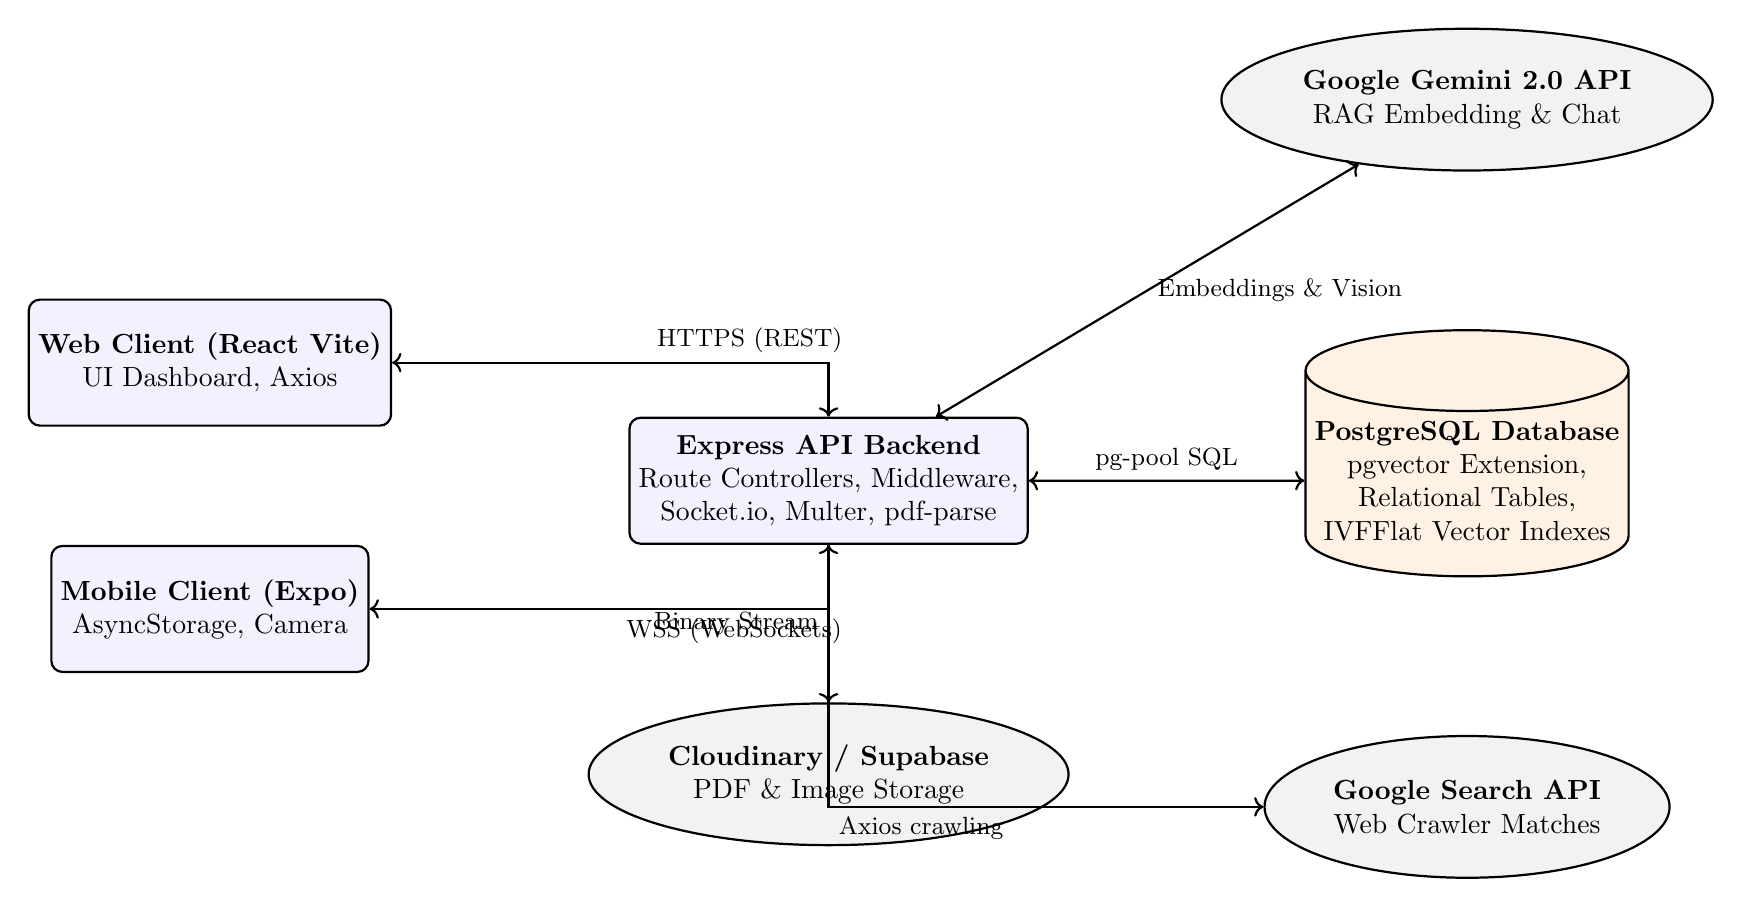
\begin{tikzpicture}[
    node distance=1.5cm and 2cm,
    box/.style={rectangle, draw, rounded corners, align=center, minimum width=3.5cm, minimum height=1.6cm, fill=blue!5, thick},
    db/.style={cylinder, draw, shape border rotate=90, aspect=0.25, align=center, minimum width=3.0cm, minimum height=2.5cm, fill=orange!10, thick},
    cloud/.style={ellipse, draw, align=center, minimum width=3.2cm, minimum height=1.8cm, fill=gray!10, thick},
    arrow/.style={-{Stealth[scale=1.2]}, thick}
]

% Nodes
\node[box] (webclient) {\textbf{Web Client (React Vite)}\\UI Dashboard, Axios};
\node[box, below=of webclient] (mobileclient) {\textbf{Mobile Client (Expo)}\\AsyncStorage, Camera};
\node[box, right=of webclient, xshift=1cm, yshift=-1.5cm] (backend) {\textbf{Express API Backend}\\Route Controllers, Middleware,\\Socket.io, Multer, pdf-parse};
\node[db, right=of backend, xshift=1.5cm] (postgres) {\textbf{PostgreSQL Database}\\pgvector Extension,\\Relational Tables,\\IVFFlat Vector Indexes};
\node[cloud, below=of backend, yshift=-0.5cm] (cloudinary) {\textbf{Cloudinary / Supabase}\\PDF \& Image Storage};
\node[cloud, above=of postgres, yshift=0.5cm] (gemini) {\textbf{Google Gemini 2.0 API}\\RAG Embedding \& Chat};
\node[cloud, below=of postgres, yshift=-0.5cm] (crawler) {\textbf{Google Search API}\\Web Crawler Matches};

% Connections
\draw[arrow, <->] (webclient) -| node[above, xshift=-1cm, font=\small] {HTTPS (REST)} (backend);
\draw[arrow, <->] (mobileclient) -| node[below, xshift=-1.2cm, font=\small] {WSS (WebSockets)} (backend);
\draw[arrow, <->] (backend) -- node[above, font=\small] {pg-pool SQL} (postgres);
\draw[arrow, ->] (backend) -- node[left, font=\small] {Binary Stream} (cloudinary);
\draw[arrow, <->] (backend) -- node[right, font=\small] {Embeddings \& Vision} (gemini);
\draw[arrow, ->] (backend) |- node[below right, font=\small] {Axios crawling} (crawler);

\end{tikzpicture}%
}
\caption{Detailed NoteHub Hardware and Software Architecture}
\label{fig:detailed_architecture}
\end{figure}

\section{MATHEMATICAL MODEL}
The core logic of NoteHub is built around mathematical definitions that enable document indexing, similarity searches, and rate limiting.

\subsection{Jaccard Similarity for Lexical Plagiarism Check}
The Winnowing algorithm converts raw normalized text strings into a set of integers representing fingerprint hashes. Let $A$ be the shingle set of hashes from the uploaded PDF document, and $B$ be the shingle set of hashes of a note already stored in the database. The lexical similarity index $J(A, B)$ is defined as:
\begin{equation}
J(A, B) = \frac{|A \cap B|}{|A \cup B|} = \frac{|A \cap B|}{|A| + |B| - |A \cap B|}
\end{equation}
The system rejects the note and flags it as plagiarized if:
\begin{equation}
J(A, B) \ge \theta_{\text{lexical}} \quad (\text{where } \theta_{\text{lexical}} = 0.40)
\end{equation}

\subsection{Hamming Distance for SimHash Near-Duplicate Checking}
To handle paraphrase modifications, the system computes a 64-bit SimHash. The text is split into terms $T$, and each term is assigned a weight $w_i$. Let $h(t_i)$ be a 64-bit standard hash of term $t_i$. The SimHash vector $\mathbf{V} = [v_0, v_1, \dots, v_{63}]$ is computed by:
\begin{equation}
v_j = \sum_{i=1}^{m} w_i \cdot \text{sign}(h(t_i)_j) \quad \text{where } \text{sign}(x) = \begin{cases} 1 & \text{if the } j\text{-th bit is } 1 \\ -1 & \text{if the } j\text{-th bit is } 0 \end{cases}
\end{equation}
The final 64-bit fingerprint hash $F = [f_0, f_1, \dots, f_{63}]$ is defined as:
\begin{equation}
f_j = \begin{cases} 1 & \text{if } v_j > 0 \\ 0 & \text{if } v_j \le 0 \end{cases}
\end{equation}
The Hamming distance between the new fingerprint $F_1$ and database fingerprint $F_2$ is:
\begin{equation}
\text{HammingDistance}(F_1, F_2) = \sum_{j=0}^{63} (f_{1,j} \oplus f_{2,j}) = \text{popcount}(F_1 \oplus F_2)
\end{equation}
Near-duplicates are flagged when:
\begin{equation}
\text{HammingDistance}(F_1, F_2) \le \theta_{\text{semantic}} \quad (\text{where } \theta_{\text{semantic}} = 3)
\end{equation}

\subsection{Cosine Similarity for pgvector RAG matches}
Natural language search and RAG contexts require calculating semantic distance. Text chunks are embedded into 1536-dimensional vectors. Let $\mathbf{q}$ be the query vector, and $\mathbf{d}$ be the chunk embedding vector. The cosine similarity is:
\begin{equation}
\text{CosineSimilarity}(\mathbf{q}, \mathbf{d}) = \frac{\mathbf{q} \cdot \mathbf{d}}{\|\mathbf{q}\| \|\mathbf{d}\|} = \frac{\sum_{i=1}^{1536} q_i d_i}{\sqrt{\sum_{i=1}^{1536} q_i^2} \sqrt{\sum_{i=1}^{1536} d_i^2}}
\end{equation}
The pgvector extension uses the distance operator \texttt{<=>}, which evaluates $1 - \text{CosineSimilarity}$. Chunks are selected when:
\begin{equation}
1 - (\mathbf{q} \cdot \mathbf{d}) / (\|\mathbf{q}\| \|\mathbf{d}\|) \le 1 - \alpha \quad (\text{where } \alpha = 0.75)
\end{equation}

\subsection{Token Bucket Rate Limiting Algorithm}
API endpoints are protected from overload using the Token Bucket abstraction. A bucket has maximum token limit $B$. Tokens accumulate at refill rate $r$ per second. The number of active tokens $T(t)$ for client $k$ is:
\begin{equation}
T_k(t) = \min(B, T_k(t_0) + r(t - t_0) - C)
\end{equation}
If $T_k(t) < 1$, the request is blocked, throwing an HTTP 429 error.

\subsection{Score and Points Model}
User points are modeled by a linear point system:
\begin{equation}
\text{Points}(u) = 50 \cdot N_{\text{verified}}(u) + 20 \cdot H_{\text{resolved}}(u) + 10 \cdot Q_{\ge 80\%}(u)
\end{equation}
where $N_{\text{verified}}$ is notes uploaded, $H_{\text{resolved}}$ is peer help requests resolved, and $Q_{\ge 80\%}$ is quizzes completed with a score above 80\%.

\section{SYSTEM FLOW DIAGRAM}
The flow diagram illustrates the sequential pipeline a document undergoes during the upload process. The document must pass through distinct validation gates before being permanently stored and published.

\begin{figure}[H]
\centering
\resizebox{!}{0.7\textheight}{%
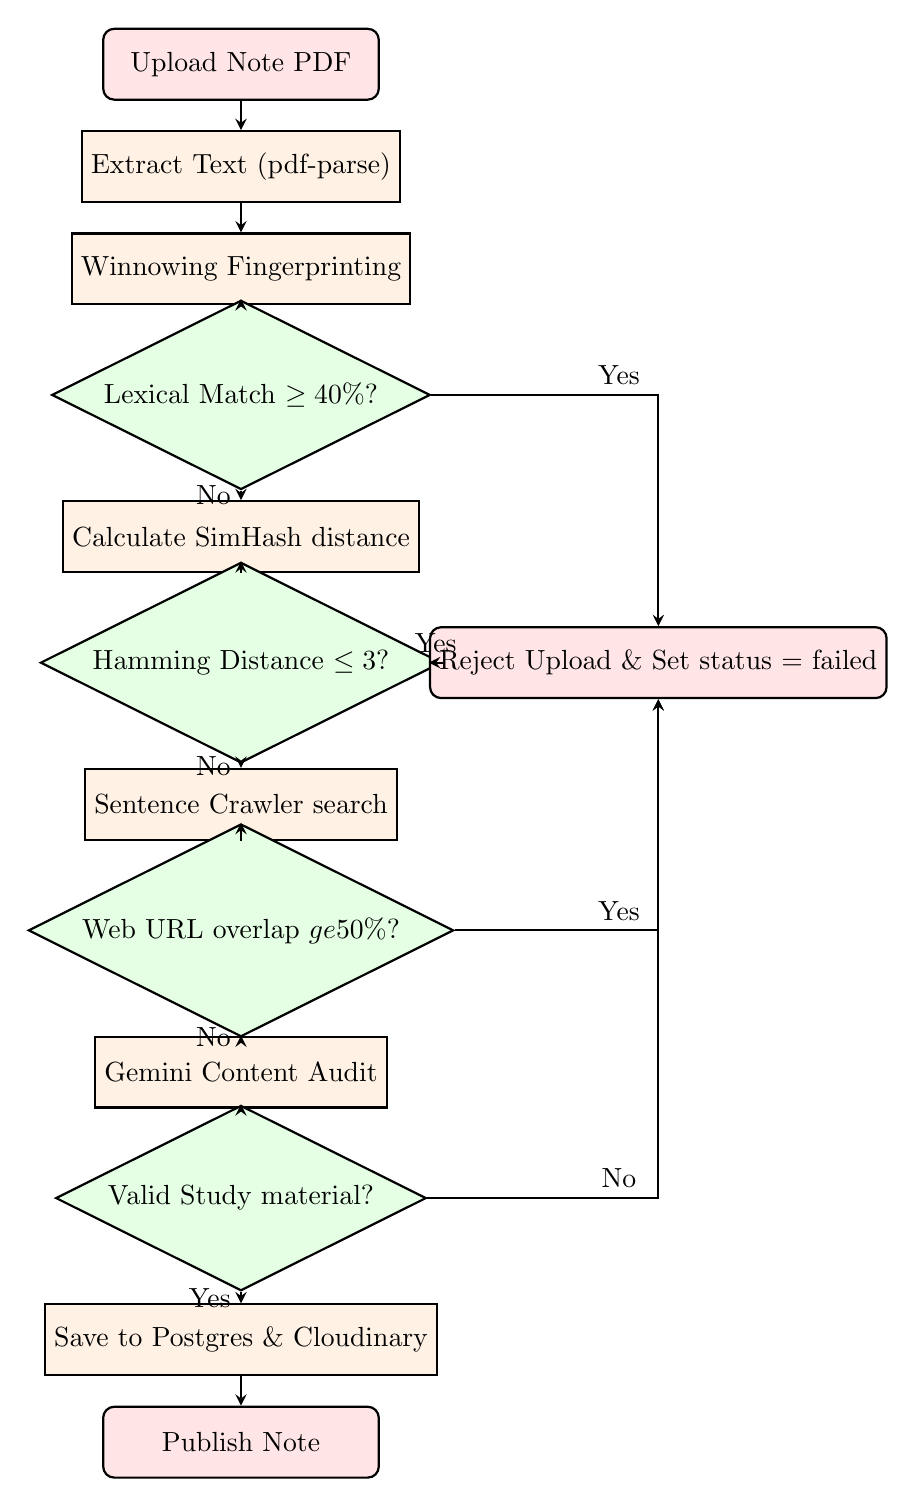
\begin{tikzpicture}[
    node distance=1.3cm,
    startstop/.style={rectangle, rounded corners, minimum width=3.5cm, minimum height=0.9cm, text centered, draw, fill=red!10, thick},
    process/.style={rectangle, minimum width=3.5cm, minimum height=0.9cm, text centered, draw, fill=orange!10, thick},
    decision/.style={diamond, aspect=2, minimum width=3.5cm, minimum height=1.0cm, text centered, draw, fill=green!10, thick},
    arrow/.style={thick,->,>=stealth}
]

% Nodes
\node (start) [startstop] {Upload Note PDF};
\node (extract) [process, below of=start] {Extract Text (pdf-parse)};
\node (winnow) [process, below of=extract] {Winnowing Fingerprinting};
\node (dec1) [decision, below of=winnow, yshift=-0.3cm] {Lexical Match $\ge 40\%?$};
\node (simhash) [process, below of=dec1, yshift=-0.5cm] {Calculate SimHash distance};
\node (dec2) [decision, below of=simhash, yshift=-0.3cm] {Hamming Distance $\le 3$?};
\node (crawler) [process, below of=dec2, yshift=-0.5cm] {Sentence Crawler search};
\node (dec3) [decision, below of=crawler, yshift=-0.3cm] {Web URL overlap $ge 50\%?$};
\node (gemini) [process, below of=dec3, yshift=-0.5cm] {Gemini Content Audit};
\node (dec4) [decision, below of=gemini, yshift=-0.3cm] {Valid Study material?};
\node (save) [process, below of=dec4, yshift=-0.5cm] {Save to Postgres \& Cloudinary};
\node (end) [startstop, below of=save] {Publish Note};
\node (reject) [startstop, right of=dec2, xshift=4cm] {Reject Upload \& Set status = failed};

% Connections
\draw [arrow] (start) -- (extract);
\draw [arrow] (extract) -- (winnow);
\draw [arrow] (winnow) -- (dec1);
\draw [arrow] (dec1) -- node[anchor=east] {No} (simhash);
\draw [arrow] (dec1) -| node[anchor=south, xshift=-0.5cm] {Yes} (reject);
\draw [arrow] (simhash) -- (dec2);
\draw [arrow] (dec2) -- node[anchor=east] {No} (crawler);
\draw [arrow] (dec2) -- node[anchor=south] {Yes} (reject);
\draw [arrow] (crawler) -- (dec3);
\draw [arrow] (dec3) -- node[anchor=east] {No} (gemini);
\draw [arrow] (dec3) -| node[anchor=south, xshift=-0.5cm] {Yes} (reject);
\draw [arrow] (gemini) -- (dec4);
\draw [arrow] (dec4) -- node[anchor=east] {Yes} (save);
\draw [arrow] (dec4) -| node[anchor=south, xshift=-0.5cm] {No} (reject);
\draw [arrow] (save) -- (end);

\end{tikzpicture}%
}
\caption{Document Ingestion and Multi-Gate Verification Pipeline Flow}
\label{fig:pipeline_flow}
\end{figure}

The pipeline begins when the student uploads a document. The server processes the upload asynchronously. If the document similarity checks trigger a pass, it is committed to storage and points are updated. Otherwise, the note is marked as rejected, preventing clutter.

\section{ER DIAGRAM}
The Entity-Relationship model specifies the logical database schema for NoteHub, detailing tables, column types, keys, and foreign relational bindings.

\begin{figure}[H]
\centering
\resizebox{\textwidth}{!}{%
\begin{tikzpicture}[
    node distance=1.5cm and 2.5cm,
    entity/.style={rectangle, draw, rounded corners=2pt, align=left, minimum width=3.5cm, fill=yellow!10, thick},
    relation/.style={draw, -{Stealth[scale=1.2]}, thick}
]

% Entities
\node[entity] (users) {
\textbf{users}\\
\hline
\underline{id} (UUID) [PK]\\
email (VARCHAR)\\
name (VARCHAR)\\
points (INTEGER)\\
role (VARCHAR)
};

\node[entity, right=of users, xshift=1.5cm] (notes) {
\textbf{notes}\\
\hline
\underline{id} (UUID) [PK]\\
title (VARCHAR)\\
file\_url (VARCHAR)\\
uploader\_id (UUID) [FK]\\
status (VARCHAR)\\
subject\_id (UUID) [FK]
};

\node[entity, below=of notes, yshift=-0.5cm] (embeddings) {
\textbf{note\_embeddings}\\
\hline
\underline{id} (UUID) [PK]\\
note\_id (UUID) [FK]\\
chunk\_index (INT)\\
content (TEXT)\\
embedding (VECTOR(1536))
};

\node[entity, below=of users, yshift=-0.5cm] (messages) {
\textbf{messages}\\
\hline
\underline{id} (UUID) [PK]\\
room\_id (UUID) [FK]\\
sender\_id (UUID) [FK]\\
content (TEXT)\\
timestamp (TIMESTAMP)
};

\node[entity, right=of notes, xshift=1.5cm] (rooms) {
\textbf{study\_rooms}\\
\hline
\underline{id} (UUID) [PK]\\
name (VARCHAR)\\
subject\_id (UUID) [FK]\\
creator\_id (UUID) [FK]
};

% Connections (1 to Many relations)
\draw[relation] (users) -- node[above, font=\small] {1:N} (notes);
\draw[relation] (notes) -- node[right, font=\small] {1:N} (embeddings);
\draw[relation] (users) -- node[left, font=\small] {1:N} (messages);
\draw[relation] (rooms) |- node[below, xshift=1cm, font=\small] {1:N} (messages);
\draw[relation] (users) -- node[above, font=\small] {1:N} (rooms);

\end{tikzpicture}%
}
\caption{NoteHub Entity-Relationship (ER) Schema Diagram}
\label{fig:er_diagram}
\end{figure}

The database architecture leverages PostgreSQL primary keys and indexing. The \texttt{note\_embeddings} table is separate from the metadata to optimize similarity search.

\section{DATA FLOW DIAGRAMS}
Data Flow Diagrams model the movement of data elements through external entities, processes, and internal databases.

\subsection{Level 0 DFD (Context Level)}
At Context Level 0, the NoteHub application is treated as a single process, showing external entities and data stores.

\begin{figure}[H]
\centering
\resizebox{0.8\textwidth}{!}{%
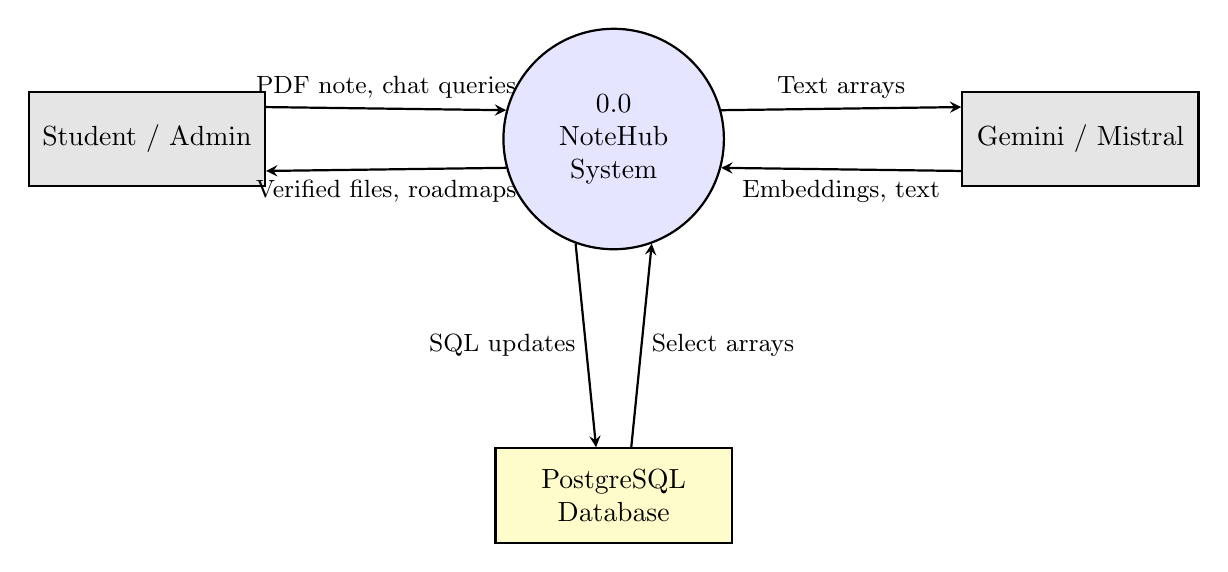
\begin{tikzpicture}[
    node distance=2.5cm,
    external/.style={rectangle, draw, minimum width=3.0cm, minimum height=1.2cm, fill=gray!20, thick, align=center},
    process/.style={circle, draw, minimum size=2.8cm, fill=blue!10, thick, align=center},
    datastore/.style={rectangle, draw, minimum width=3.0cm, minimum height=1.2cm, fill=yellow!20, thick, align=center},
    arrow/.style={thick,->,>=stealth}
]

% Nodes
\node (student) [external] {Student / Admin};
\node (sys) [process, right=of student, xshift=0.5cm] {0.0\\NoteHub\\System};
\node (ai) [external, right=of sys, xshift=0.5cm] {Gemini / Mistral};
\node (db) [datastore, below=of sys] {PostgreSQL\\Database};

% Connections
\draw [arrow] (student.15) -- node[above, font=\small] {PDF note, chat queries} (sys.165);
\draw [arrow] (sys.195) -- node[below, font=\small] {Verified files, roadmaps} (student.345);
\draw [arrow] (sys.15) -- node[above, font=\small] {Text arrays} (ai.165);
\draw [arrow] (ai.195) -- node[below, font=\small] {Embeddings, text} (sys.345);
\draw [arrow] (sys.250) -- node[left, font=\small] {SQL updates} (db.110);
\draw [arrow] (db.70) -- node[right, font=\small] {Select arrays} (sys.290);

\end{tikzpicture}%
}
\caption{Context Level Data Flow Diagram (Level 0)}
\label{fig:dfd0_ch5}
\end{figure}

\subsection{Level 1 DFD (Process Level)}
Level 1 DFD decomposes the system into core sub-processes: Authentication, Note Ingestion, Plagiarism, Advisor, and Collaboration.

\begin{figure}[H]
\centering
\resizebox{\textwidth}{!}{%
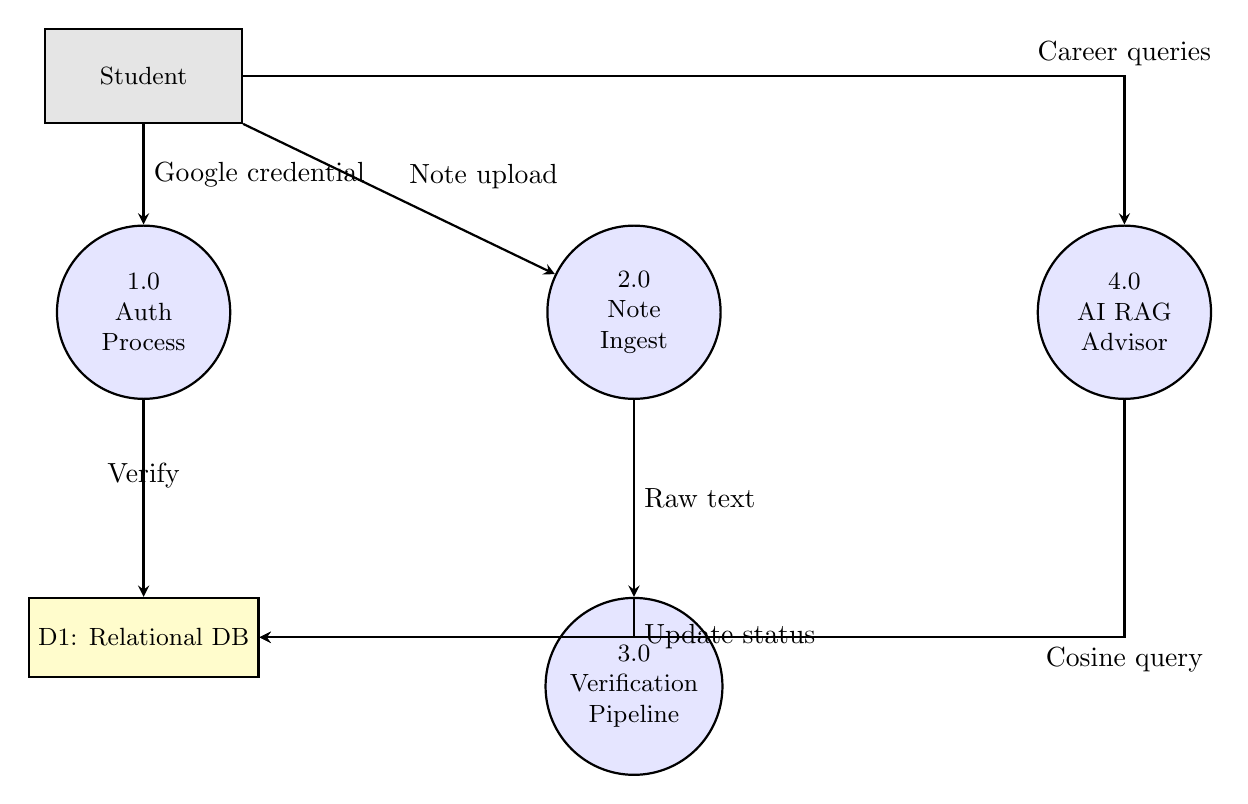
\begin{tikzpicture}[
    node distance=1.5cm and 2.5cm,
    process/.style={circle, draw, minimum size=2.2cm, fill=blue!10, thick, align=center, font=\small},
    datastore/.style={rectangle, draw, minimum width=2.5cm, minimum height=1cm, fill=yellow!20, thick, align=center, font=\small},
    external/.style={rectangle, draw, minimum width=2.5cm, minimum height=1.2cm, fill=gray!20, thick, align=center, font=\small},
    arrow/.style={thick,->,>=stealth}
]

% Nodes
\node (student) [external] {Student};
\node (auth) [process, below of=student, yshift=-1.5cm] {1.0\\Auth\\Process};
\node (ingest) [process, right=of auth, xshift=1.5cm] {2.0\\Note\\Ingest};
\node (verify) [process, below=of ingest, yshift=-1.0cm] {3.0\\Verification\\Pipeline};
\node (rag) [process, right=of ingest, xshift=1.5cm] {4.0\\AI RAG\\Advisor};
\node (db) [datastore, below=of auth, yshift=-1.0cm] {D1: Relational DB};

% Arrows
\draw [arrow] (student) -- node[right] {Google credential} (auth);
\draw [arrow] (auth) -- node[above] {Verify} (db);
\draw [arrow] (student) -- node[above right] {Note upload} (ingest);
\draw [arrow] (ingest) -- node[right] {Raw text} (verify);
\draw [arrow] (verify) |- node[below right, yshift=0.3cm] {Update status} (db);
\draw [arrow] (student) -| node[above] {Career queries} (rag);
\draw [arrow] (rag) |- node[below] {Cosine query} (db);

\end{tikzpicture}%
}
\caption{Process Level Data Flow Diagram (Level 1)}
\label{fig:dfd1}
\end{figure}

\subsection{Level 2 DFD (Decomposed Verification Pipeline)}
Level 2 DFD details the sub-processes of the Plagiarism and Verification Pipeline (Process 3.0).

\begin{figure}[H]
\centering
\resizebox{\textwidth}{!}{%
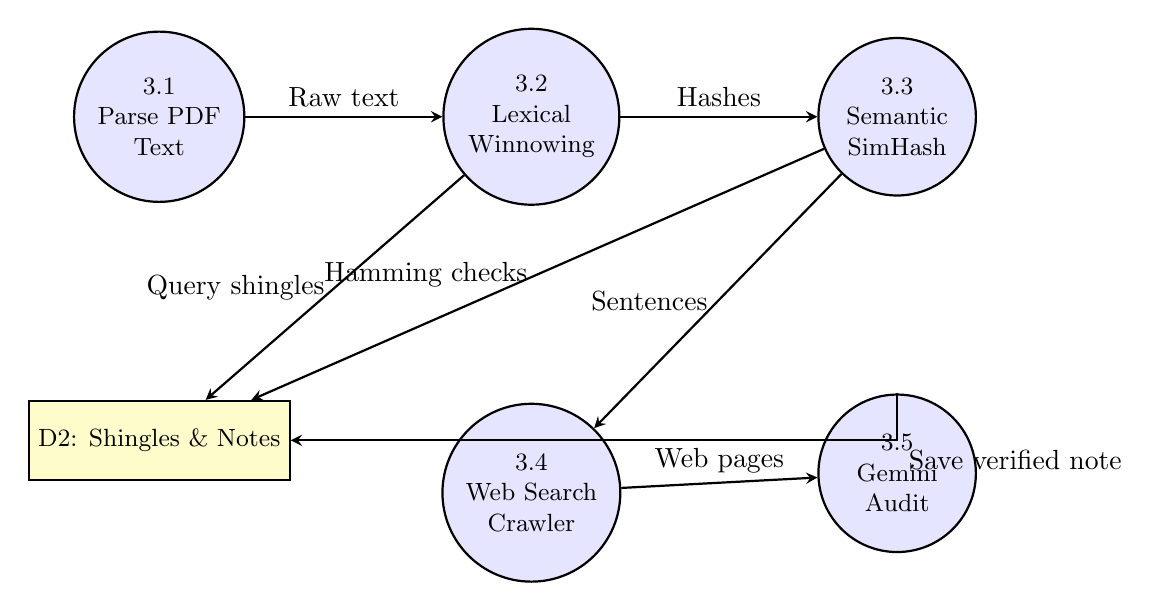
\begin{tikzpicture}[
    node distance=1.5cm and 2.0cm,
    process/.style={circle, draw, minimum size=2.0cm, fill=blue!10, thick, align=center, font=\small},
    datastore/.style={rectangle, draw, minimum width=2.5cm, minimum height=1cm, fill=yellow!20, thick, align=center, font=\small},
    external/.style={rectangle, draw, minimum width=2.5cm, minimum height=1.2cm, fill=gray!20, thick, align=center, font=\small},
    arrow/.style={thick,->,>=stealth}
]

% Nodes
\node (input) [process] {3.1\\Parse PDF\\Text};
\node (winnow) [process, right=of input, xshift=0.5cm] {3.2\\Lexical\\Winnowing};
\node (simhash) [process, right=of winnow, xshift=0.5cm] {3.3\\Semantic\\SimHash};
\node (crawler) [process, below=of winnow, yshift=-1.0cm] {3.4\\Web Search\\Crawler};
\node (gemini) [process, below=of simhash, yshift=-1.0cm] {3.5\\Gemini\\Audit};
\node (db) [datastore, below=of input, yshift=-1.0cm] {D2: Shingles \& Notes};

% Connections
\draw [arrow] (input) -- node[above] {Raw text} (winnow);
\draw [arrow] (winnow) -- node[above] {Hashes} (simhash);
\draw [arrow] (winnow) -- node[left] {Query shingles} (db);
\draw [arrow] (simhash) -- node[left] {Hamming checks} (db);
\draw [arrow] (simhash) -- node[left] {Sentences} (crawler);
\draw [arrow] (crawler) -- node[above] {Web pages} (gemini);
\draw [arrow] (gemini) |- node[below, xshift=1.5cm] {Save verified note} (db);

\end{tikzpicture}%
}
\caption{Decomposed Verification Data Flow Diagram (Level 2)}
\label{fig:dfd2}
\end{figure}

\section{UML DIAGRAMS}
Unified Modeling Language (UML) diagrams specify the object-oriented structure, class operations, execution timelines, and deployments.

\subsection{Use Case Diagram}
The Use Case Diagram defines the interactions between platform actors and functional boundaries.

\begin{figure}[H]
\centering
\resizebox{!}{0.65\textheight}{%
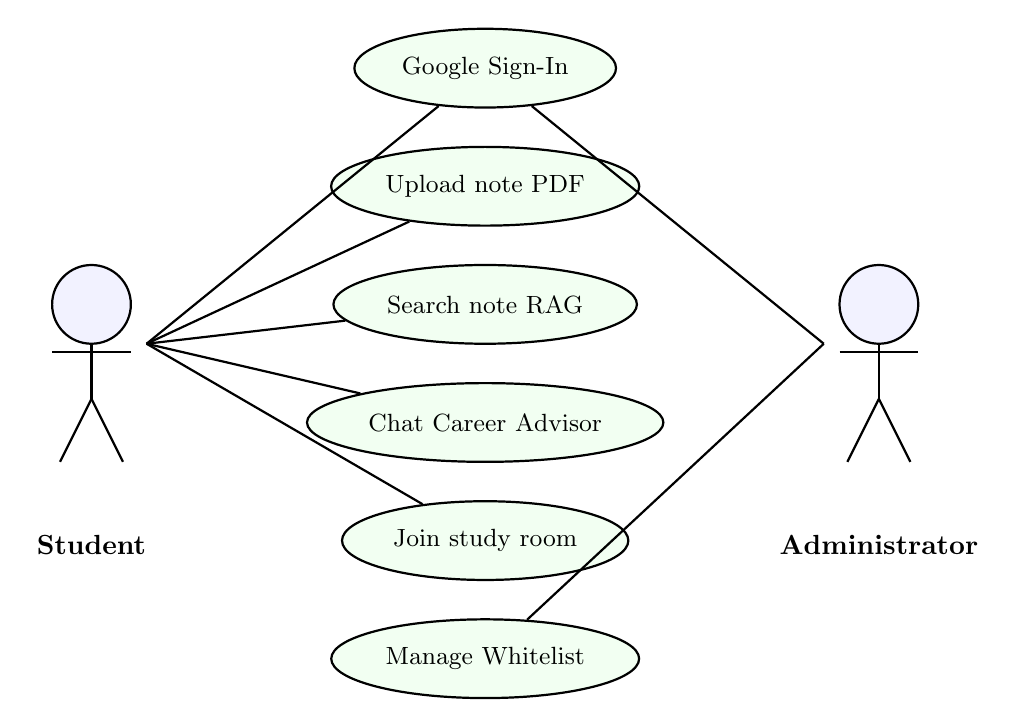
\begin{tikzpicture}[
    actor/.style={draw, circle, minimum size=1cm, fill=blue!5, thick},
    usecase/.style={ellipse, draw, fill=green!5, minimum width=3cm, minimum height=1cm, thick, align=center, font=\small},
    relation/.style={draw, thick}
]

% Student Actor
\node[actor] (student) at (-4, 0) {};
\draw[thick] (student.south) -- (-4, -1.2);
\draw[thick] (-4.5, -0.6) -- (-3.5, -0.6);
\draw[thick] (-4, -1.2) -- (-4.4, -2.0);
\draw[thick] (-4, -1.2) -- (-3.6, -2.0);
\node[below=of student, yshift=-1.3cm] {\textbf{Student}};

% Admin Actor
\node[actor] (admin) at (6, 0) {};
\draw[thick] (admin.south) -- (6, -1.2);
\draw[thick] (5.5, -0.6) -- (6.5, -0.6);
\draw[thick] (6, -1.2) -- (5.6, -2.0);
\draw[thick] (6, -1.2) -- (6.4, -2.0);
\node[below=of admin, yshift=-1.3cm] {\textbf{Administrator}};

% Use Cases
\node[usecase] (uc1) at (1, 3) {Google Sign-In};
\node[usecase] (uc2) at (1, 1.5) {Upload note PDF};
\node[usecase] (uc3) at (1, 0) {Search note RAG};
\node[usecase] (uc4) at (1, -1.5) {Chat Career Advisor};
\node[usecase] (uc5) at (1, -3) {Join study room};
\node[usecase] (uc6) at (1, -4.5) {Manage Whitelist};

% Connections
\draw[relation] (-3.3, -0.5) -- (uc1);
\draw[relation] (-3.3, -0.5) -- (uc2);
\draw[relation] (-3.3, -0.5) -- (uc3);
\draw[relation] (-3.3, -0.5) -- (uc4);
\draw[relation] (-3.3, -0.5) -- (uc5);
\draw[relation] (5.3, -0.5) -- (uc1);
\draw[relation] (5.3, -0.5) -- (uc6);

\end{tikzpicture}%
}
\caption{UML Use Case Diagram}
\label{fig:use_case}
\end{figure}

\subsection{Class Diagram}
The Class Diagram models the attributes and operations of the backend routing and business controllers.

\begin{figure}[H]
\centering
\resizebox{\textwidth}{!}{%
\begin{tikzpicture}[
    class/.style={rectangle, draw, minimum width=4.5cm, fill=yellow!5, thick, align=left, font=\small}
]

% UserController
\node[class] (userCtrl) {
\textbf{UserController}\\
\hline
- dbPool: pg.Pool\\
+ registerUser(req, res)\\
+ loginGoogle(req, res)\\
+ getAchievements(req, res)
};

% NoteController
\node[class, right=of userCtrl, xshift=1cm] (noteCtrl) {
\textbf{NoteController}\\
\hline
- storageClient: Supabase\\
+ uploadNote(req, res)\\
+ searchSemantic(req, res)\\
+ getNoteDetails(req, res)
};

% PlagiarismEngine
\node[class, below=of noteCtrl, yshift=-0.5cm] (plagEngine) {
\textbf{PlagiarismEngine}\\
\hline
- kgramSize: int = 20\\
- windowSize: int = 15\\
+ runWinnowing(text): int[]\\
+ calculateSimHash(text): long\\
+ queryCrawler(sentences): URL[]
};

% Connections
\draw[thick, ->] (noteCtrl) -- (plagEngine);

\end{tikzpicture}%
}
\caption{UML Class Diagram}
\label{fig:class_diagram}
\end{figure}

\subsection{Sequence Diagram}
The Sequence Diagram traces the operational steps during note upload and plagiarism checking.

\begin{figure}[H]
\centering
\resizebox{\textwidth}{!}{%
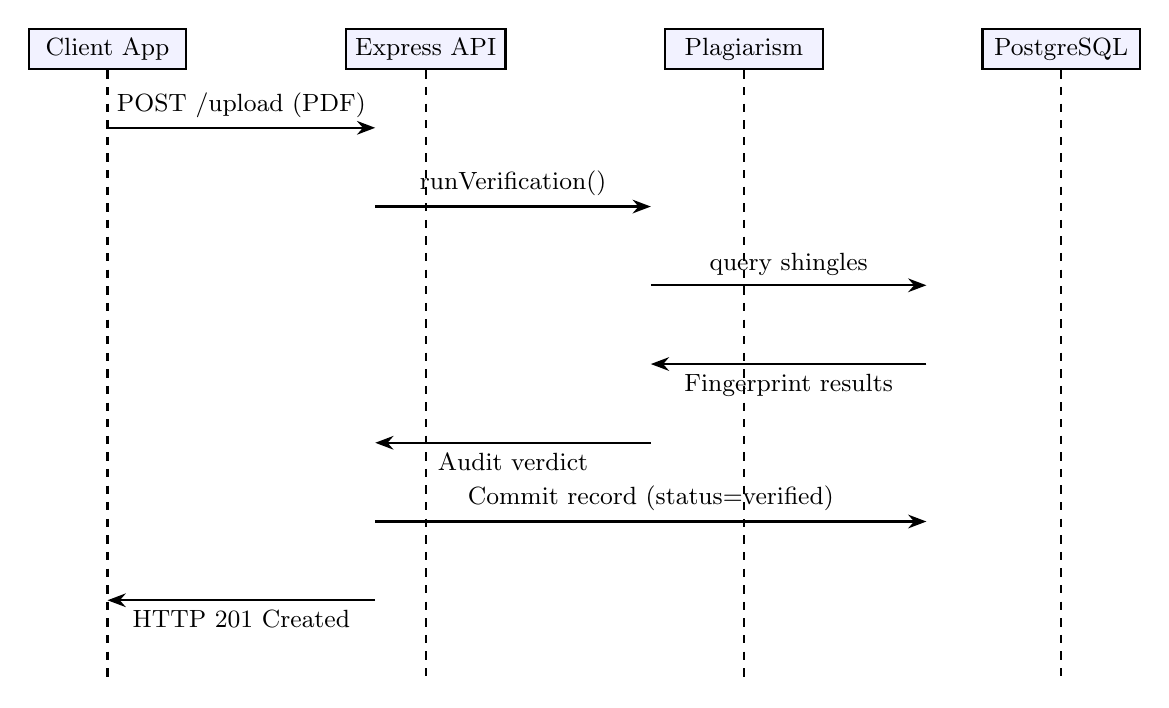
\begin{tikzpicture}[
    lifeline/.style={rectangle, draw, minimum width=2cm, fill=blue!5, thick, align=center, font=\small},
    line/.style={dashed, thick},
    arrow/.style={-{Stealth}, thick}
]

% Lifelines
\node[lifeline] (client) {Client App};
\node[lifeline, right=of client, xshift=1cm] (backend) {Express API};
\node[lifeline, right=of backend, xshift=1cm] (engine) {Plagiarism};
\node[lifeline, right=of engine, xshift=1cm] (db) {PostgreSQL};

% Timelines
\draw[line] (client) -- (client |- 0,-8);
\draw[line] (backend) -- (backend |- 0,-8);
\draw[line] (engine) -- (engine |- 0,-8);
\draw[line] (db) -- (db |- 0,-8);

% Actions
\draw[arrow] (0,-1) -- node[above, font=\small] {POST /upload (PDF)} (3.4,-1);
\draw[arrow] (3.4,-2) -- node[above, font=\small] {runVerification()} (6.9,-2);
\draw[arrow] (6.9,-3) -- node[above, font=\small] {query shingles} (10.4,-3);
\draw[arrow] (10.4,-4) -- node[below, font=\small] {Fingerprint results} (6.9,-4);
\draw[arrow] (6.9,-5) -- node[below, font=\small] {Audit verdict} (3.4,-5);
\draw[arrow] (3.4,-6) -- node[above, font=\small] {Commit record (status=verified)} (10.4,-6);
\draw[arrow] (3.4,-7) -- node[below, font=\small] {HTTP 201 Created} (0,-7);

\end{tikzpicture}%
}
\caption{UML Sequence Diagram for Note Upload Pipeline}
\label{fig:sequence_diagram}
\end{figure}

\subsection{Collaboration Diagram}
The Collaboration Diagram highlights the structural interactions and message numbering between client, server, and storage.

\begin{figure}[H]
\centering
\resizebox{0.85\textwidth}{!}{%
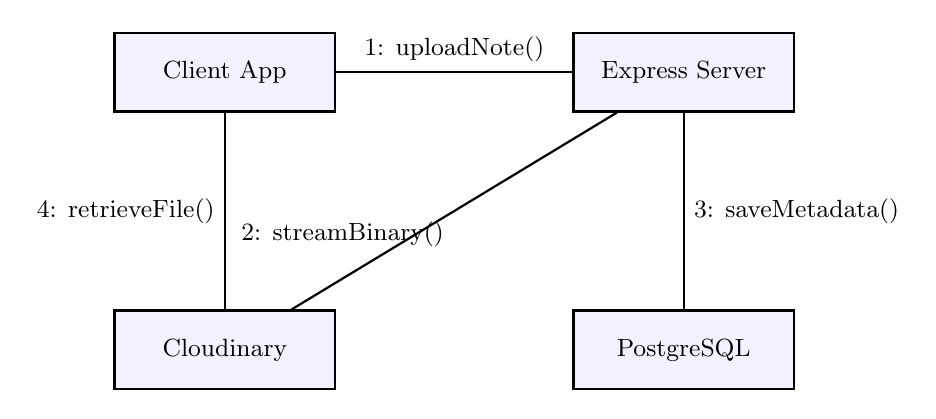
\begin{tikzpicture}[
    object/.style={rectangle, draw, minimum width=2.8cm, minimum height=1cm, fill=blue!5, thick, align=center, font=\small},
    arrow/.style={-{Stealth}, thick}
]

% Nodes
\node[object] (client) {Client App};
\node[object, right=of client, xshift=2cm] (api) {Express Server};
\node[object, below=of api, yshift=-1.5cm] (db) {PostgreSQL};
\node[object, left=of db, xshift=-2cm] (storage) {Cloudinary};

% Messages
\draw[thick] (client) -- node[above, font=\small] {1: uploadNote()} (api);
\draw[thick] (api) -- node[right, font=\small] {3: saveMetadata()} (db);
\draw[thick] (api) -- node[below left, font=\small] {2: streamBinary()} (storage);
\draw[thick] (client) -- node[left, font=\small] {4: retrieveFile()} (storage);

\end{tikzpicture}%
}
\caption{UML Collaboration Diagram}
\label{fig:collaboration_diagram}
\end{figure}

\subsection{Activity Diagram}
The Activity Diagram maps the process states of real-time messaging verification in Socket namespaces.

\begin{figure}[H]
\centering
\resizebox{!}{0.65\textheight}{%
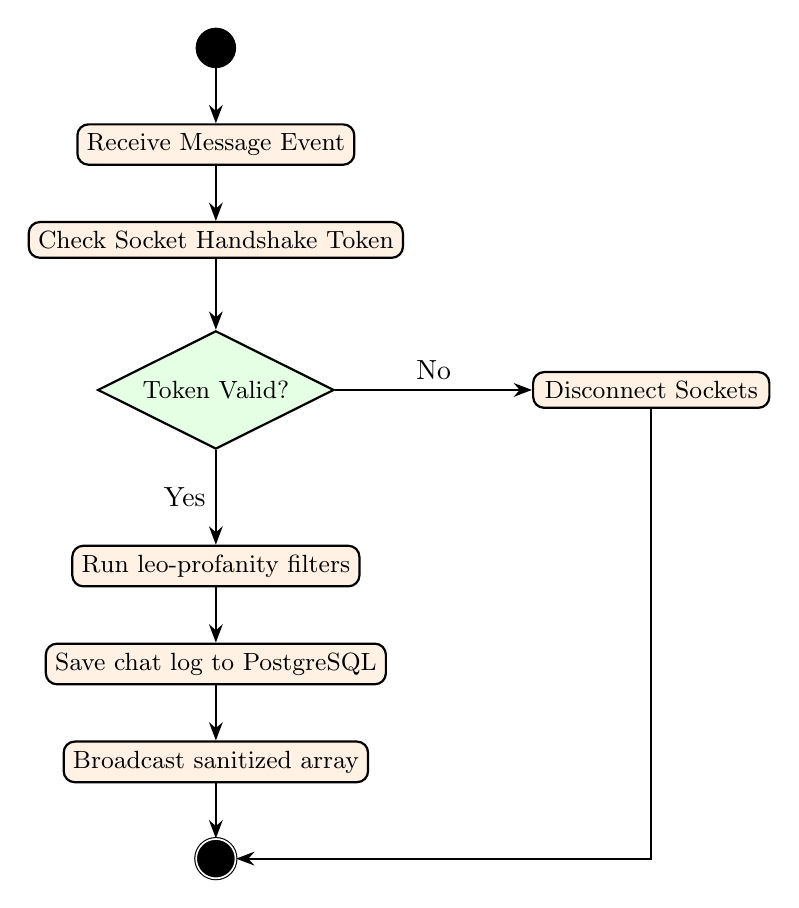
\begin{tikzpicture}[
    state/.style={rectangle, draw, rounded corners, minimum width=3cm, fill=orange!10, thick, align=center, font=\small},
    decision/.style={diamond, draw, aspect=2, fill=green!10, thick, align=center, font=\small},
    arrow/.style={-{Stealth}, thick}
]

% Nodes
\node[circle, draw, fill=black, minimum size=0.5cm] (start) at (0,0) {};
\node[state, below=of start, yshift=0.3cm] (recv) {Receive Message Event};
\node[state, below=of recv, yshift=0.3cm] (jwt) {Check Socket Handshake Token};
\node[decision, below=of jwt, yshift=0.1cm] (dec1) {Token Valid?};
\node[state, below=of dec1, yshift=-0.2cm] (filter) {Run leo-profanity filters};
\node[state, below=of filter, yshift=0.3cm] (db) {Save chat log to PostgreSQL};
\node[state, below=of db, yshift=0.3cm] (broadcast) {Broadcast sanitized array};
\node[circle, draw, double, fill=black, minimum size=0.5cm, below=of broadcast, yshift=0.3cm] (end) {};
\node[state, right=of dec1, xshift=1.5cm] (reject) {Disconnect Sockets};

% Connections
\draw[arrow] (start) -- (recv);
\draw[arrow] (recv) -- (jwt);
\draw[arrow] (jwt) -- (dec1);
\draw[arrow] (dec1) -- node[left] {Yes} (filter);
\draw[arrow] (dec1) -- node[above] {No} (reject);
\draw[arrow] (filter) -- (db);
\draw[arrow] (db) -- (broadcast);
\draw[arrow] (broadcast) -- (end);
\draw[arrow] (reject) |- (end);

\end{tikzpicture}%
}
\caption{UML Activity Diagram for Socket Chat Moderation}
\label{fig:activity_diagram}
\end{figure}

\subsection{State Chart Diagram}
The State Chart Diagram models the states of Note upload.

\begin{figure}[H]
\centering
\resizebox{\textwidth}{!}{%
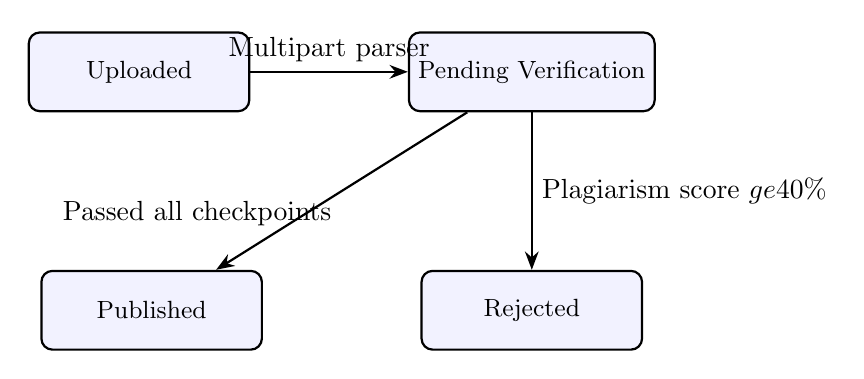
\begin{tikzpicture}[
    state/.style={rectangle, draw, rounded corners, minimum width=2.8cm, minimum height=1cm, fill=blue!5, thick, align=center, font=\small},
    arrow/.style={-{Stealth}, thick}
]

% Nodes
\node[state] (uploaded) {Uploaded};
\node[state, right=of uploaded, xshift=1cm] (pending) {Pending Verification};
\node[state, below=of pending, yshift=-1cm] (failed) {Rejected};
\node[state, left=of failed, xshift=-1cm] (verified) {Published};

% Connections
\draw[arrow] (uploaded) -- node[above] {Multipart parser} (pending);
\draw[arrow] (pending) -- node[right] {Plagiarism score $ge 40\%$} (failed);
\draw[arrow] (pending) -- node[below left] {Passed all checkpoints} (verified);

\end{tikzpicture}%
}
\caption{UML State Chart Diagram for Document Entity}
\label{fig:statechart_diagram}
\end{figure}

\subsection{Component Diagram}
The Component Diagram details the module packages on client web, mobile, and Express APIs.

\begin{figure}[H]
\centering
\resizebox{\textwidth}{!}{%
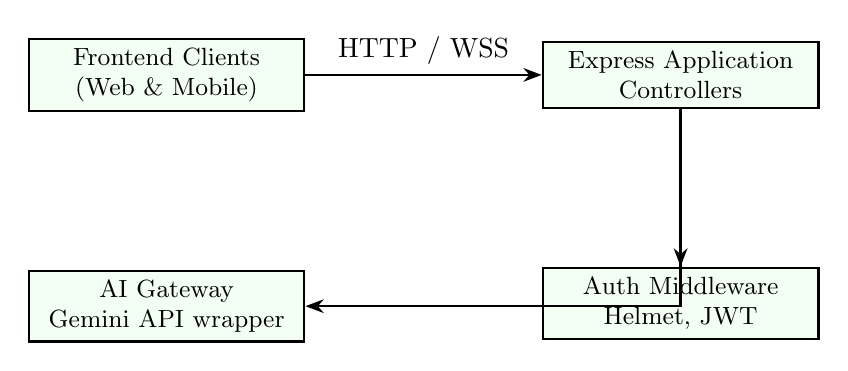
\begin{tikzpicture}[
    component/.style={rectangle, draw, minimum width=3.5cm, fill=green!5, thick, align=center, font=\small},
    interface/.style={circle, draw, minimum size=0.3cm, fill=white, thick},
    arrow/.style={draw, -{Stealth}, thick}
]

% Components
\node[component] (frontend) {Frontend Clients\\(Web \& Mobile)};
\node[component, right=of frontend, xshift=2cm] (backend) {Express Application\\Controllers};
\node[component, below=of backend, yshift=-1cm] (security) {Auth Middleware\\Helmet, JWT};
\node[component, below=of frontend, yshift=-1cm] (ai) {AI Gateway\\Gemini API wrapper};

% Connectors
\draw[arrow] (frontend) -- node[above] {HTTP / WSS} (backend);
\draw[arrow] (backend) -- (security);
\draw[arrow] (backend) |- (ai);

\end{tikzpicture}%
}
\caption{UML Component Diagram}
\label{fig:component_diagram}
\end{figure}

\subsection{Deployment Diagram}
The Deployment Diagram maps the physical hosts (Vercel, Render Docker containers, PostgreSQL databases, Cloudinary clusters).

\begin{figure}[H]
\centering
\resizebox{\textwidth}{!}{%
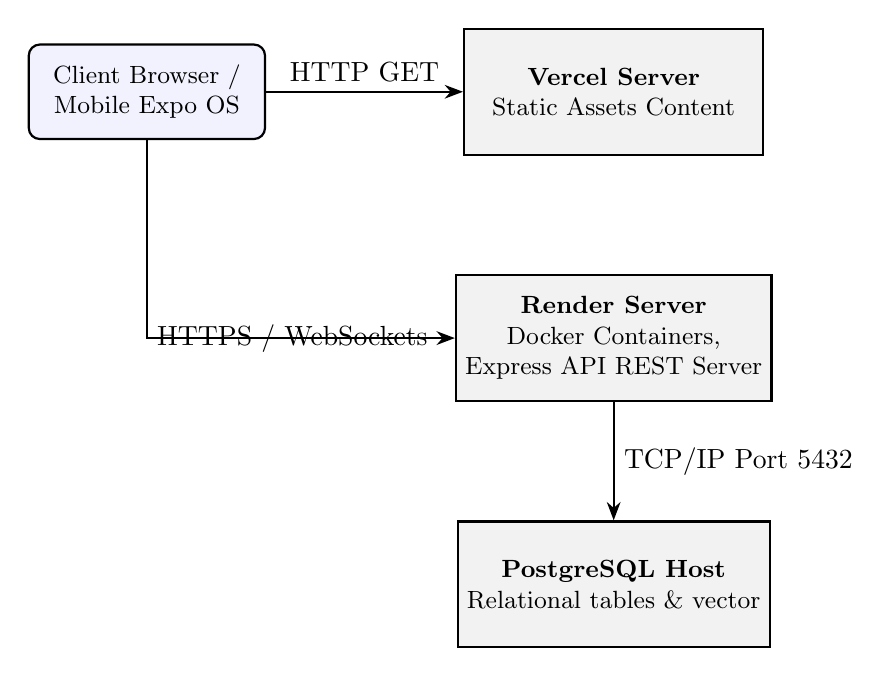
\begin{tikzpicture}[
    node/.style={rectangle, draw, minimum width=3.8cm, minimum height=1.6cm, fill=gray!10, thick, align=center, font=\small},
    device/.style={rectangle, draw, rounded corners, minimum width=3.0cm, minimum height=1.2cm, fill=blue!5, thick, align=center, font=\small},
    arrow/.style={draw, -{Stealth}, thick}
]

% Nodes
\node[device] (client) {Client Browser /\\Mobile Expo OS};
\node[node, right=of client, xshift=1.5cm] (vercel) {\textbf{Vercel Server}\\Static Assets Content};
\node[node, below=of vercel, yshift=-0.5cm] (render) {\textbf{Render Server}\\Docker Containers,\\Express API REST Server};
\node[node, below=of render, yshift=-0.5cm] (postgres) {\textbf{PostgreSQL Host}\\Relational tables \& vector};

% Connections
\draw[arrow] (client) -- node[above] {HTTP GET} (vercel);
\draw[arrow] (client) |- node[below right, yshift=0.3cm] {HTTPS / WebSockets} (render);
\draw[arrow] (render) -- node[right] {TCP/IP Port 5432} (postgres);

\end{tikzpicture}%
}
\caption{UML Physical Deployment Diagram}
\label{fig:deployment_diagram}
\end{figure}

\subsection{Package Diagram}
The Package Diagram segments the repository codebase into backend routes, controller files, middleware wrappers, and configurations.

\begin{figure}[H]
\centering
\resizebox{\textwidth}{!}{%
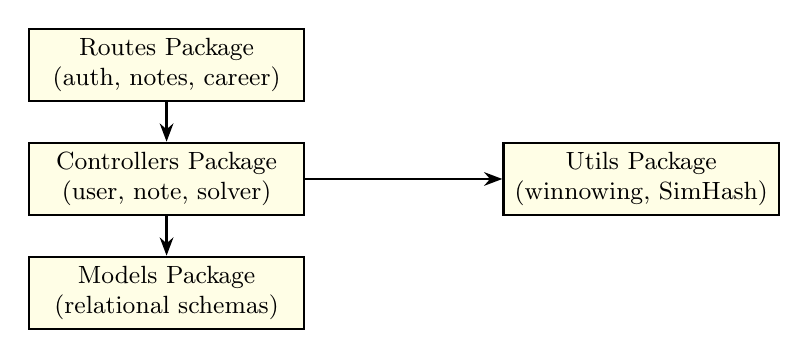
\begin{tikzpicture}[
    package/.style={rectangle, draw, minimum width=3.5cm, fill=yellow!10, thick, align=center, font=\small},
    arrow/.style={draw, -{Stealth}, thick}
]

% Packages
\node[package] (routes) {Routes Package\\(auth, notes, career)};
\node[package, below=of routes, yshift=0.5cm] (ctrl) {Controllers Package\\(user, note, solver)};
\node[package, below=of ctrl, yshift=0.5cm] (model) {Models Package\\(relational schemas)};
\node[package, right=of ctrl, xshift=1.5cm] (utils) {Utils Package\\(winnowing, SimHash)};

% Connections
\draw[arrow] (routes) -- (ctrl);
\draw[arrow] (ctrl) -- (model);
\draw[arrow] (ctrl) -- (utils);

\end{tikzpicture}%
}
\caption{UML Package Structure Diagram}
\label{fig:package_diagram}
\end{figure}

The packages diagram (Figure~\ref{fig:package_diagram}) represents the directory setup, isolating routing endpoints from controller operations and utility math modules, which guarantees model-view-controller separation.
\chapter{SYSTEM IMPLEMENTATION}
\rule{\textwidth}{1pt}
\paragraph{}
\section{PROJECT IMPLEMENTATION OVERVIEW}

System implementation is the phase in which the abstract architecture, interface designs, mathematical models, and process flows documented in previous chapters are translated into a concrete, executable software system. The development of NoteHub was structured around a modern, iterative lifecycle utilizing Agile Scrum principles. This approach allowed the development team to iteratively build, test, and refine modules in a controlled manner, ensuring that the critical core engines---such as the Winnowing plagiarism checker and the pgvector-powered career advisor---were validated before building secondary client features.

Development was conducted over a four-phase schedule corresponding to four 2-week sprints. The team prioritized database schema design and file management first (Sprint 1), followed by the core API pipeline and plagiarism checker (Sprint 2), the RAG pipeline and AI career advisor (Sprint 3), and finally, real-time collaboration, user interfaces, gamification, and cloud deployment (Sprint 4).

To maintain code quality and prevent integration conflicts in the monorepo codebase, Git version control was strictly enforced using a feature-branch workflow. The workflow rules were defined as follows:
\begin{itemize}
    \item \textbf{Main Branch (production):} Represents the stable, production-ready release of NoteHub. Direct commits to the main branch were blocked.
    \item \textbf{Development Branch (dev):} Serves as the primary integration branch where new features are combined and tested.
    \item \textbf{Feature Branches (feature/\textit{name}):} Developers worked on isolated features (e.g., \texttt{feature/auth}, \texttt{feature/plagiarism-engine}, \texttt{feature/rag-chat}) branched off the \texttt{dev} branch.
    \item \textbf{Pull Requests (PR):} Merging into the dev branch required a pull request, passing local verification checks (ESLint compilation and unit tests), and receiving approval from at least one other developer.
\end{itemize}

The implementation process followed six distinct milestones, detailed chronologically below.

% ---------------------------------------------------------
\subsection{Step 1 — Development Environment Setup}

The first milestone was establishing a uniform and reproducible development environment across all developers' local machines. This mitigated the common problem of environmental inconsistencies (\textit{"it works on my machine"}).

On the backend, Node.js v20 LTS was selected as the JavaScript runtime to ensure access to modern async/await syntax and ES modules. The project was initialized with \texttt{npm init}, and the basic middleware packages were configured: \texttt{express} for handling routes, \texttt{cors} to manage cross-origin request permissions, and \texttt{dotenv} to safely extract database credentials and private API keys from local configuration files.

On the frontend, Vite was used to bootstrap the React application using a TypeScript configuration. Vite was chosen for its fast Hot Module Replacement (HMR) and lightweight dev server, which avoids the long bundling delays of traditional Webpack. Core UI utility packages, such as \texttt{lucide-react} for icons and Tailwind CSS for utility styling, were added. Global workspace directories were structured to isolate components, custom routes, database migrations, and utilities.

% ---------------------------------------------------------
\subsection{Step 2 — Database Initialisation}

The second milestone was the configuration and setup of the PostgreSQL database. NoteHub relies heavily on PostgreSQL's robust relational features and support for high-dimensional vector search via the \texttt{pgvector} extension.

A comprehensive schema initialization script, \texttt{init.sql}, was written to define all tables, fields, constraints, and relationships. First, the \texttt{pgvector} extension was enabled using \texttt{CREATE EXTENSION IF NOT EXISTS vector}. Next, core tables representing users, notes, shingles, and embeddings were constructed. 

Primary keys were index-configured, and foreign keys were defined with cascading rules to prevent orphaned records (for example, deleting a user automatically cascades to their leaderboard standing). To optimize the performance of similarity searches on high-dimensional data, special indices were configured: standard B-Tree indexes on textual search columns (such as Note categories) and a specialized \texttt{IVFFlat} index on vector columns to accelerate nearest-neighbor retrieval.

% ---------------------------------------------------------
\subsection{Step 3 — Backend API Implementation}

With the database established, the Express.js application was structured as a collection of decoupled route controllers. All REST API endpoints were registered under the \texttt{/api/v1} prefix, separating public endpoints (such as public note searches and login) from protected routes (such as note uploading, profile modifications, and career advisory).

A custom authentication middleware, \texttt{authenticateToken}, was written to intercept requests to protected endpoints. This middleware extracts the JSON Web Token (JWT) from the incoming authorization header, decodes the user identity, checks the signature against the server's secret key, and appends the user information to the request object. 

To process file uploads, \texttt{multer} was integrated as a middleware on the note upload route. When a client submits a PDF note, Multer buffers the binary file in server memory, permitting the backend to immediately extract textual strings using \texttt{pdf-parse} and compute hashes. On completion, the binary file is streamed to Supabase Cloud Storage, and the metadata is saved to PostgreSQL.

% ---------------------------------------------------------
\subsection{Step 4 — Frontend Client Implementation}

The presentation layer was implemented as a responsive React Single Page Application (SPA). Global application state, specifically the logged-in student's user profile, JWT, and authentication status, is maintained using a React Context Provider (\texttt{AuthContext}). This prevents the antipattern of prop-drilling.

Client-side routing is managed through a lightweight hash-based router that dynamically mounts top-level view modules based on the window location. Key layouts (such as the Note Cards grid, Leaderboard ranking tables, and Group Chat panel) were constructed with responsive Tailwind classes, ensuring usability on both mobile screens and desktop monitors.

The Note Upload Modal was designed as a finite state machine with animated scanning phases. While the backend performs calculations, the frontend transitions through states: \texttt{uploading} $\rightarrow$ \texttt{extracting\_text} $\rightarrow$ \texttt{checking\_internal\_similarity} $\rightarrow$ \texttt{crawling\_web\_sources} $\rightarrow$ \texttt{generating\_ai\_report} $\rightarrow$ \texttt{done}.

% ---------------------------------------------------------
\subsection{Step 5 — Integration and Testing}

Once both the client and server components reached functional parity, they were integrated. A local Docker-compose environment was configured to run PostgreSQL, the Express server, and the Vite client together.

Integration testing focused heavily on the synchronization of the plagiarism checker and the RAG pipeline. Automated test scripts using Jest and Supertest were executed to simulate concurrent note uploads, verifying that the server correctly computed Jaccard similarities, logged embedding vectors in pgvector, rejected overlapping shingles, and properly formatted the JSON responses.

Manual User Acceptance Testing (UAT) was conducted using Chrome and Firefox developer tool consoles to debug layout alignments, WebSocket chat connections under simulated packet loss, and error boundaries for API failures (such as token expiration).

% ---------------------------------------------------------
\subsection{Step 6 — Cloud Deployment and Production Setup}

The final step was deploying the functional monorepo to production cloud infrastructure. A production-ready configuration was established:
\begin{itemize}
    \item \textbf{Frontend Hosting:} The Vite application was compiled into static HTML/JS/CSS assets using \texttt{npm run build}. The output directory was deployed to Vercel, which provides fast global delivery via its CDN.
    \item \textbf{Backend Hosting:} The Node.js Express server was packaged into a Docker container and deployed to Render. The service was configured to auto-scale based on memory utilization.
    \item \textbf{Database Hosting:} A managed PostgreSQL database was provisioned on Supabase, and the \texttt{init.sql} script was run to construct the tables and enable \texttt{pgvector}.
    \item \textbf{Cloud File Storage:} Supabase Storage buckets were created with policies that restrict direct write permissions, ensuring all PDF uploads are routed through the backend verifications first.
\end{itemize}

\subsection{Implementation Steps Summary}

Table~\ref{tab:impl_steps} summarizes the tasks, outputs, and sprint schedule followed during the implementation phase.

\begin{table}[htbp]
\centering
\renewcommand{\arraystretch}{1.5}
\caption{NoteHub Implementation Steps Summary}
\label{tab:impl_steps}
\resizebox{\textwidth}{!}{%
\begin{tabular}{|c|l|l|l|p{4.5cm}|}
\hline
\textbf{Step} & \textbf{Activity} & \textbf{Key Outputs} & \textbf{Sprint} & \textbf{Developer Role} \\
\hline
1 & Env Setup & Project directory structure, Git configuration & Pre-IT & Lead Developer \\
\hline
2 & DB Setup & init.sql, pgvector installation, indices & Sprint 1 & Database Engineer \\
\hline
3 & API Routes & Auth handlers, upload route, message router & Sprint 1-2 & Backend Developer \\
\hline
4 & UI Screens & Notes Grid, Chat Panel, Career Chat Interface & Sprint 3 & Frontend Developer \\
\hline
5 & Engines & Winnowing custom algorithm, RAG pgvector helper & Sprint 2-3 & ML/Algorithm Specialist \\
\hline
6 & Deployment & Render Docker deploy, Vercel build, CDN routing & Sprint 4 & DevOps Engineer \\
\hline
\end{tabular}%
}
\end{table}

\newpage
\section{IMPLEMENTED SYSTEM ARCHITECTURE}

The physical implementation of NoteHub is structured around a \textbf{three-tier client--server architecture}. The separation of concerns between presentation, business logic, and database persistence is maintained across all modules. This design guarantees that database operations are isolated from user-facing screens and that the server acts as an authoritative controller.

\subsection{Architecture Diagram}

Figure~\ref{fig:arch_diagram} illustrates the physical deployment topology of the implemented NoteHub system, tracing HTTP REST traffic, real-time WebSocket events, database query protocols, and third-party API connections.

\begin{figure}[htbp]
\centering
\resizebox{\textwidth}{!}{%
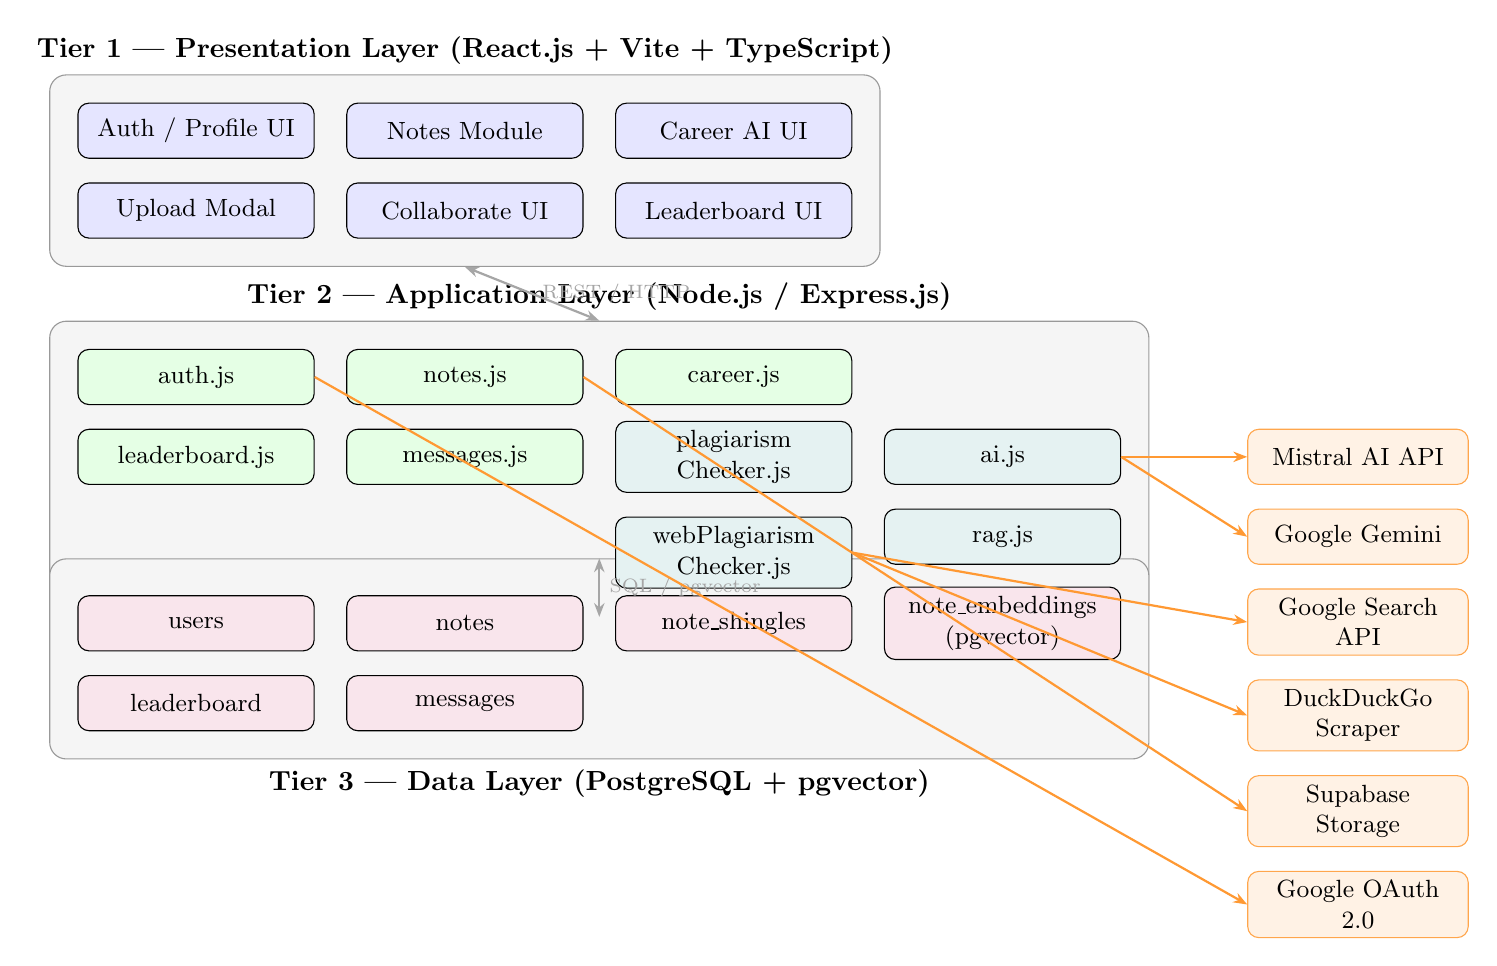
\begin{tikzpicture}[
    node distance = 0.6cm and 1.0cm,
    box/.style     = {rectangle, draw=black, rounded corners=4pt,
                      minimum width=3.0cm, minimum height=0.7cm,
                      font=\small, fill=white, align=center},
    tier/.style    = {rectangle, draw=black!40, rounded corners=6pt,
                      inner sep=10pt, fill=gray!8},
    ext/.style     = {rectangle, draw=orange!70, rounded corners=4pt,
                      minimum width=2.8cm, minimum height=0.7cm,
                      font=\small, fill=orange!10, align=center},
    arrow/.style   = {-{Stealth[length=5pt]}, thick},
    darrow/.style  = {{Stealth[length=5pt]}-{Stealth[length=5pt]}, thick, gray!70}
]

%% -- Tier 1: Frontend --------------------------------------
\node[box, fill=blue!10] (auth_ui)   {Auth / Profile UI};
\node[box, fill=blue!10, right=0.4cm of auth_ui]  (notes_ui)   {Notes Module};
\node[box, fill=blue!10, right=0.4cm of notes_ui] (career_ui)  {Career AI UI};
\node[box, fill=blue!10, below=0.3cm of auth_ui]  (upload_ui)  {Upload Modal};
\node[box, fill=blue!10, right=0.4cm of upload_ui](collab_ui)  {Collaborate UI};
\node[box, fill=blue!10, right=0.4cm of collab_ui](leader_ui)  {Leaderboard UI};

\begin{scope}[on background layer]
  \node[tier, fit=(auth_ui)(notes_ui)(career_ui)(upload_ui)(collab_ui)(leader_ui),
        label=above:{\textbf{Tier 1 — Presentation Layer (React.js + Vite + TypeScript)}}]
        (tier1) {};
\end{scope}

%% -- Tier 2: Backend ---------------------------------------
\node[box, fill=green!10, below=1.4cm of upload_ui] (auth_rt)   {auth.js};
\node[box, fill=green!10, right=0.4cm of auth_rt]   (notes_rt)  {notes.js};
\node[box, fill=green!10, right=0.4cm of notes_rt]  (career_rt) {career.js};
\node[box, fill=green!10, below=0.3cm of auth_rt]   (leader_rt) {leaderboard.js};
\node[box, fill=green!10, right=0.4cm of leader_rt] (msg_rt)    {messages.js};

\node[box, fill=teal!10, right=0.4cm of msg_rt]     (plag_ut)   {plagiarism\\Checker.js};
\node[box, fill=teal!10, below=0.3cm of plag_ut]    (webp_ut)   {webPlagiarism\\Checker.js};
\node[box, fill=teal!10, right=0.4cm of plag_ut]    (ai_ut)     {ai.js};
\node[box, fill=teal!10, below=0.3cm of ai_ut]      (rag_ut)    {rag.js};

\begin{scope}[on background layer]
  \node[tier, fit=(auth_rt)(notes_rt)(career_rt)(leader_rt)(msg_rt)(plag_ut)(webp_ut)(ai_ut)(rag_ut),
        label=above:{\textbf{Tier 2 — Application Layer (Node.js / Express.js)}}]
        (tier2) {};
\end{scope}

%% -- Tier 3: Database --------------------------------------
\node[box, fill=purple!10, below=1.4cm of leader_rt] (db_users)  {users};
\node[box, fill=purple!10, right=0.4cm of db_users]  (db_notes)  {notes};
\node[box, fill=purple!10, right=0.4cm of db_notes]  (db_shin)   {note\_shingles};
\node[box, fill=purple!10, right=0.4cm of db_shin]   (db_emb)    {note\_embeddings\\(pgvector)};
\node[box, fill=purple!10, below=0.3cm of db_users]  (db_lb)     {leaderboard};
\node[box, fill=purple!10, right=0.4cm of db_lb]     (db_msg)    {messages};

\begin{scope}[on background layer]
  \node[tier, fit=(db_users)(db_notes)(db_shin)(db_emb)(db_lb)(db_msg),
        label=below:{\textbf{Tier 3 — Data Layer (PostgreSQL + pgvector)}}]
        (tier3) {};
\end{scope}

%% -- External Services -------------------------------------
\node[ext, right=1.6cm of ai_ut]   (mistral)  {Mistral AI API};
\node[ext, below=0.3cm of mistral] (gemini)   {Google Gemini};
\node[ext, below=0.3cm of gemini]  (gsearch)  {Google Search\\API};
\node[ext, below=0.3cm of gsearch] (ddg)      {DuckDuckGo\\Scraper};
\node[ext, below=0.3cm of ddg]     (supabase) {Supabase\\Storage};
\node[ext, below=0.3cm of supabase](goauth)   {Google OAuth\\2.0};

%% -- Arrows: Frontend <-> Backend ----------------------------
\draw[darrow] (tier1.south) -- node[right, font=\scriptsize]{REST / HTTP} (tier2.north);

%% -- Arrows: Backend <-> Database ----------------------------
\draw[darrow] (tier2.south) -- node[right, font=\scriptsize]{SQL / pgvector} (tier3.north);

%% -- Arrows: Backend -> External ----------------------------
\draw[arrow, orange!80] (ai_ut.east)   -- (mistral.west);
\draw[arrow, orange!80] (ai_ut.east)   -- (gemini.west);
\draw[arrow, orange!80] (webp_ut.east) -- (gsearch.west);
\draw[arrow, orange!80] (webp_ut.east) -- (ddg.west);
\draw[arrow, orange!80] (notes_rt.east)-- (supabase.west);
\draw[arrow, orange!80] (auth_rt.east) -- (goauth.west);

\end{tikzpicture}%
}
\caption{NoteHub Implemented System Architecture (Three-Tier with External Services)}
\label{fig:arch_diagram}
\end{figure}

% ---------------------------------------------------------
\subsection{Tier 1 — Presentation Layer}

The presentation layer is the user's entry point. Developed using React.js 18, Vite, and TypeScript, it is compiled as a static Single Page Application (SPA). To maintain a smooth user experience, all API calls to the backend are asynchronous (using Axios) and do not trigger page refreshes.

The UI utilizes dynamic layouts that resize automatically based on the user's device. CSS styles are handled using Tailwind CSS utility definitions. When the application loads, Vite mounts the main \texttt{App.tsx} component which acts as the layout shell, rendering navigation menus and checking if a valid JWT is saved in the browser's session storage.

If the user is logged in, the \texttt{AuthContext} is populated, making the user's profile available to all views. Communication with the backend is abstracted into \texttt{src/services/api.js}, which automatically attaches the JWT token to the authorization headers of outgoing requests.

% ---------------------------------------------------------
\subsection{Tier 2 — Application Layer}

The business logic of NoteHub runs on a Node.js Express server. It handles routing, coordinates file parsing, executes the plagiarism logic, and structures database operations.

Rather than maintaining a single large server file, routes are segmented into dedicated controllers (such as \texttt{routes/auth.js} and \texttt{routes/notes.js}) and mounted as Express sub-routers. Heavy computing operations, such as computing hashes or comparing fingerprint arrays, are isolated into helper utility modules in the \texttt{utils/} directory. This structure allows the main server routing layer to remain clean.

To handle real-time chat, a Socket.io server is attached directly to the Node.js HTTP server. This allows client connections to bypass the standard REST request pipeline, establishing persistent, bidirectional TCP tunnels for fast message delivery.

% ---------------------------------------------------------
\subsection{Tier 3 — Data Layer}

The database layer runs on PostgreSQL 15. The database structures all note metadata, student profiles, shingles, and chat history. To perform Retrieval-Augmented Generation, pgvector stores 1536-dimensional float vector embeddings generated by the LLM embedding API. 

The backend application establishes connection pooling via the \texttt{pg.Pool} client. Connection pooling allows the backend to keep a pool of reusable database connections active, reducing the CPU and latency overhead of establishing a new TCP handshake for every single API request.

Database indexes are split into:
\begin{itemize}
    \item \textbf{B-Tree Indexes:} Configured on foreign keys (such as \texttt{uploader\_id} and \texttt{user\_id}) and string search inputs (such as Note subjects and academic departments).
    \item \textbf{Vector Indexes (IVFFlat):} Set up on the embedding vector column on the \texttt{note\_embeddings} table to allow fast cosine distance queries.
\end{itemize}

% ---------------------------------------------------------
\subsection{External Service Integration}

NoteHub relies on several third-party cloud APIs to enrich its feature set:
\begin{enumerate}
    \item \textbf{Mistral AI API:} The primary LLM provider. Used to evaluate document quality during verification and generate answers for the career advisor.
    \item \textbf{Google Gemini API:} The backup LLM provider. Used when the Mistral service is unavailable or rate-limited.
    \item \textbf{Google Custom Search API:} Used during web plagiarism checks. The backend submits extracted sentences to Google to find online matches.
    \item \textbf{DuckDuckGo HTML Scraper:} A backup search mechanism that scrapes search results if the Google API limit is reached.
    \item \textbf{Supabase Storage:} Hosts PDF files. When a note is verified, the file is saved to Supabase, which returns a public URL.
    \item \textbf{Google OAuth 2.0 API:} Handles social authentication, verifying the student's university identity.
\end{enumerate}

% ---------------------------------------------------------
\subsection{Project Directory Structure}

The NoteHub codebase is organized as a monorepo containing both the frontend client code and backend server code. This layout makes it easy to share configurations and run local tests. The folder directory structure is shown below:

\begin{verbatim}
Notehub/
|-- .env                        # Root configuration file
|-- init.sql                    # Database tables and constraints
|-- package.json                # Frontend dependencies
|-- vite.config.ts              # Vite bundle configuration
|-- src/                        # Frontend source folder
|   |-- components/             # Reusable UI parts
|   |   |-- UploadModal.tsx     # Note upload workflow
|   |   |-- LeaderboardTable.tsx# Student ranking display
|   |   `-- NotePreviewModal.tsx# PDF reader and report viewer
|   |-- modules/                # Core page views
|   |   |-- Notes.tsx           # Search and filter notes
|   |   |-- CareerAI.tsx        # Career advisor chat interface
|   |   |-- Collaborate.tsx     # Real-time study groups
|   |   `-- Leaderboard.tsx     # Gamified standings
|   |-- services/
|   |   `-- api.js              # Asynchronous HTTP requests
|   `-- context/
|       `-- AuthContext.tsx     # Global JWT and user state
`-- backend/
    |-- package.json            # Backend package configurations
    `-- src/
        |-- server.js           # Main Express server entry point
        |-- db.js               # PostgreSQL connection pool helper
        |-- routes/             # Express routes controllers
        |   |-- auth.js         # User registration and social login
        |   |-- notes.js        # Note uploads and database CRUD
        |   |-- career.js       # RAG pipeline routing
        |   |-- leaderboard.js  # Ranking update queries
        |   `-- messages.js     # Persistent chat records
        `-- utils/              # Computational algorithms
            |-- ai.js           # Multi-provider LLM connector
            |-- rag.js          # Vector chunking and embedding queries
            |-- plagiarismChecker.js # Rolling hash plagiarism engine
            |-- webPlagiarismChecker.js # Search API web comparison
            `-- aiVerifier.js   # Content validation logic
\end{verbatim}

\newpage
\section{DEVELOPMENT ENVIRONMENT}

To support consistent development, the workspace was configured with detailed hardware, software, and configuration files.

\subsection{Hardware and Operating System}

Table~\ref{tab:hardware} lists the minimum local development specs required to compile and run NoteHub's client and server.

\begin{table}[htbp]
\centering
\renewcommand{\arraystretch}{1.5}
\caption{Development Hardware and OS Specifications}
\label{tab:hardware}
\resizebox{\textwidth}{!}{%
\begin{tabular}{|l|l|p{8.0cm}|}
\hline
\textbf{Component} & \textbf{Specification} & \textbf{Importance to NoteHub} \\
\hline
Operating System   & Windows 11 Home (64-bit) & Standard environment matching student test machines. \\
\hline
Processor          & Intel Core i5 / AMD Ryzen 5 & Essential for fast compilation of TS files and local builds. \\
\hline
RAM                & 8 GB DDR4 & Minimum memory required to run Postgres, Node, and Vite concurrently. \\
\hline
Storage            & 256 GB SSD & Provides fast disk I/O, vital for loading node\_modules. \\
\hline
Browser            & Chrome 124 / Firefox 125 & Used to verify CSS layouts, localStorage, and WebSockets. \\
\hline
\end{tabular}%
}
\end{table}

\subsection{Development Tools and IDE}

Visual Studio Code (v1.88+) served as the unified IDE for the team. Code standards were enforced using ESLint for static script auditing and Prettier for automated syntax formatting. VS Code extensions including \texttt{TypeScript IntelliSense}, \texttt{GitLens}, and \texttt{REST Client} accelerated feature iteration. API endpoint validation was performed using Postman before writing front-end client services.

\subsection{Backend Production Dependencies}

All backend packages are configured in \texttt{backend/package.json}. Table~\ref{tab:backend_deps} details these modules.

\begin{table}[htbp]
\centering
\renewcommand{\arraystretch}{1.4}
\caption{Backend Production Dependencies}
\label{tab:backend_deps}
\resizebox{\textwidth}{!}{%
\begin{tabular}{|l|l|p{7.5cm}|}
\hline
\textbf{Package} & \textbf{Version} & \textbf{Purpose / Application} \\
\hline
\texttt{express} & \^{}4.18.2 & Core server router, registers HTTP request middleware. \\
\hline
\texttt{cors} & \^{}2.8.5 & Handles cross-origin client request credentials. \\
\hline
\texttt{dotenv} & \^{}16.4.5 & Extracts secure keys from root configuration variables. \\
\hline
\texttt{pg} & \^{}8.11.3 & Connects to PostgreSQL, manages query connection pooling. \\
\hline
\texttt{multer} & \^{}1.4.5 & Processes multipart/form-data for inbound PDF uploads. \\
\hline
\texttt{bcrypt} & \^{}5.1.1 & Hashes student passwords using salt-iterated keys. \\
\hline
\texttt{jsonwebtoken} & \^{}9.0.2 & Generates signed JWT tokens representing user identity. \\
\hline
\texttt{google-auth-library} & \^{}9.7.0 & Cryptographically validates Google authentication tokens. \\
\hline
\texttt{pdf-parse} & \^{}1.1.1 & Extracts raw text segments from binary PDF buffers. \\
\hline
\texttt{openai} & \^{}4.28.0 & Communicates with Mistral AI via OpenAI endpoint emulation. \\
\hline
\texttt{@google/generative-ai} & \^{}0.15.0 & Native client wrapper for Gemini LLM calls. \\
\hline
\texttt{socket.io} & \^{}4.7.4 & Initiates WebSocket routing for real-time study rooms. \\
\hline
\texttt{bottleneck} & \^{}2.19.5 & Prevents external API failures by rate-limiting calls. \\
\hline
\texttt{@supabase/supabase-js} & \^{}2.39.0 & Manages file uploads to Supabase cloud buckets. \\
\hline
\texttt{node-fetch} & \^{}2.7.0 & Fetches web content for search crawlers in Node.js. \\
\hline
\end{tabular}%
}
\end{table}

\subsection{Frontend Production Dependencies}

Frontend dependencies are defined in the main \texttt{package.json} file at the project root. Table~\ref{tab:frontend_deps} outlines the library structures used in the client.

\begin{table}[htbp]
\centering
\renewcommand{\arraystretch}{1.4}
\caption{Frontend Production Dependencies}
\label{tab:frontend_deps}
\resizebox{\textwidth}{!}{%
\begin{tabular}{|l|l|p{7.5cm}|}
\hline
\textbf{Package} & \textbf{Version} & \textbf{Purpose / Application} \\
\hline
\texttt{react} & \^{}18.2.0 & Component-driven client state model and user interface framework. \\
\hline
\texttt{react-dom} & \^{}18.2.0 & Renders React components to browser HTML elements. \\
\hline
\texttt{typescript} & \^{}5.2.2 & Implements strict typing for API responses and structures. \\
\hline
\texttt{vite} & \^{}5.0.0 & Dev compiler and packager for static assets. \\
\hline
\texttt{pdfjs-dist} & \^{}4.0.3 & Renders PDF file buffers directly on browser canvases. \\
\hline
\texttt{lucide-react} & \^{}0.378.0 & UI icons (shields, brains, download metrics, user ranks). \\
\hline
\texttt{tailwindcss} & \^{}3.4.1 & Utility classes for rapid UI construction and dark mode. \\
\hline
\texttt{socket.io-client} & \^{}4.7.4 & Connects client application to server WebSocket endpoints. \\
\hline
\end{tabular}%
}
\end{table}

\subsection{Environment Variables Summary}

All configuration variables are managed locally in the root \texttt{.env} file. This file contains variables defining Postgres details, Google social log client identifiers, AI authorization tokens, search query ids, and Supabase cloud access permissions.

\begin{verbatim}
# Database Configuration
POSTGRES_USER=notehub_dev_user
POSTGRES_PASSWORD=secure_postgres_pass
POSTGRES_DB=notehub_db
DB_HOST=127.0.0.1
DB_PORT=5433

# JWT Token Security Settings
JWT_SECRET=super_secret_auth_token_key_generation_algorithm
GOOGLE_CLIENT_ID=38927498273-example-client.apps.googleusercontent.com

# Artificial Intelligence API Access Keys
MISTRAL_API_KEY=mistral_large_production_secret_token
GOOGLE_API_KEY=gemini_developer_key_token_payload

# Google Programmable Custom Search
GOOGLE_SEARCH_API_KEY=custom_search_rest_api_key
GOOGLE_SEARCH_CX=search_engine_profile_id

# Cloud Resource Credentials
SUPABASE_URL=https://supabase.co/project/reference
SUPABASE_KEY=supabase_client_role_key_value
\end{verbatim}

\newpage
\section{TECHNOLOGIES AND TOOLS USED}

The technology selections for NoteHub were chosen based on execution speed, package ecosystems, developer support, and integration compatibility.

\subsection{Programming Languages}

\subsubsection*{JavaScript (Node.js)}
JavaScript is the foundation of the NoteHub server. Running Node.js v20 LTS, it utilizes an asynchronous, event-driven, single-threaded execution model. This is critical for NoteHub, where a typical file upload request requires making concurrent asynchronous outbound network calls to Supabase Storage, Google Search APIs, and LLM verification endpoints. A multi-threaded platform (such as Java or C\#) would block a thread per client request while waiting for these network responses. Node.js manages these operations concurrently using its internal event loop, maximizing throughput while minimizing CPU usage.

\subsubsection*{TypeScript}
TypeScript is used across the frontend workspace. Writing a student platform with multiple features (like note uploading, plagiarism checks, and interactive AI chats) introduces complex nested object models. TypeScript's type definitions ensure that changes to the structure of the API response (such as modifications to the JSON plagiarism report schema) are automatically checked across all frontend components at compile-time. This eliminates runtime \texttt{undefined} errors in the browser.

\subsubsection*{Structured Query Language (SQL)}
SQL is the language used to interact with PostgreSQL. Because NoteHub relies on relationships between users, uploaded documents, chat history, and gamification ranks, relational integrity is important. Parameterized SQL queries are used to prevent SQL injection vulnerabilities. PostgreSQL-specific features, such as arrays for shingles and the custom vector operators provided by pgvector, are utilized for system operations.

\subsection{Frontend Framework and CSS Engine}

\subsubsection*{React.js 18}
React is the client-side framework used to build NoteHub. It structures the application into self-contained components. React's Virtual DOM diffing algorithm is critical during note uploads, where multiple UI states (upload status, percentage rings, current step label) are updated in real-time. By calculating DOM changes in memory and batching updates to the page, React maintains a smooth 60 FPS user interface.

\subsubsection*{Tailwind CSS 3}
Tailwind CSS provides utility classes for styling. Rather than writing traditional CSS files, Tailwind styles are applied directly in JSX files. Tailwind's Just-In-Time (JIT) compiler parses the codebase at build time and compiles only the CSS classes that are actually used. This keeps production stylesheets lightweight and enables responsive dark mode styling using the \texttt{dark:} selector.

\subsection{Algorithmic and Database Extensions}

\subsubsection*{pgvector}
The \texttt{pgvector} extension is used to store text vector embeddings within PostgreSQL. In a typical relational database, searching for semantic similarity across text requires expensive full-text search indexing or running external engines (such as Elasticsearch). pgvector integrates vector storage directly into standard SQL. By using pgvector's cosine distance operator (\texttt{<=>}), NoteHub can run high-dimensional vector search queries alongside standard relational filters in a single SQL statement.

\newpage
\section{MODULE IMPLEMENTATION}

This section describes the physical implementation of the nine core modules that make up the NoteHub system. Each module section describes the implementation logic on both the frontend and backend, and provides a representative code snippet inside a \texttt{verbatim} block to illustrate the implementation pattern.

% ==========================================
\subsection{Module 1: Authentication and Profile Management}

The authentication module handles user registrations, logins, and social authorization via Google OAuth 2.0. The frontend uses the Google Login button component. On a successful login, the client receives a Google token ID and submits it to the backend endpoint \texttt{POST /api/auth/google}. 

The backend verifies the token using the official Google Auth Library. If valid, it extracts the student's name, email, and profile photo. If this is a new registration, a corresponding user row is created in the database. The server then generates a JWT containing the user ID, role, and department, signed with the server's secret key, and sends it to the client. The client stores this JWT in local storage to authorize subsequent requests.

Representative backend login token validation code is shown in Listing~\ref{lst:auth_code}:

\begin{verbatim}
// backend/src/routes/auth.js (Google Authentication Endpoint)
const router = require('express').Router();
const { OAuth2Client } = require('google-auth-library');
const jwt = require('jsonwebtoken');
const pool = require('../db');

const client = new OAuth2Client(process.env.GOOGLE_CLIENT_ID);

router.post('/google', async (req, res) => {
  const { credential } = req.body;
  try {
    const ticket = await client.verifyIdToken({
      idToken: credential,
      audience: process.env.GOOGLE_CLIENT_ID,
    });
    const payload = ticket.getPayload();
    const { email, name, picture } = payload;

    // Check if user already exists in PostgreSQL
    let userResult = await pool.query('SELECT * FROM users WHERE email = $1', [email]);
    let user = userResult.rows[0];

    if (!user) {
      // Create user with default 100 registration points
      const insertQuery = `
        INSERT INTO users (name, email, avatar_url, points, badges) 
        VALUES ($1, $2, $3, 100, '{}') RETURNING *
      `;
      const insertResult = await pool.query(insertQuery, [name, email, picture]);
      user = insertResult.rows[0];
      
      // Initialize corresponding empty leaderboard row
      await pool.query('INSERT INTO leaderboard (user_id, points) VALUES ($1, 100)', [user.id]);
    }

    // Sign identity JWT token
    const token = jwt.sign(
      { id: user.id, email: user.email, role: user.role },
      process.env.JWT_SECRET,
      { expiresIn: '7d' }
    );

    res.status(200).json({ success: true, token, user });
  } catch (error) {
    console.error('Google Auth Error:', error);
    res.status(401).json({ success: false, error: 'Invalid Google credential' });
  }
});
\end{verbatim}
\label{lst:auth_code}

% ==========================================
\subsection{Module 2: Note Management and Discovery}

This module manages note search, tag-filtering, cataloging, and document uploads. The frontend uses input elements that filter the note listings by subject and semester. 

When a student initiates an upload, the backend routes the file upload through \texttt{multer} configuration middleware. The file is saved in memory, text content is extracted using \texttt{pdf-parse}, and unique hashes are computed. The file is then uploaded to Supabase Storage. The storage service returns a public URL, which is written to the database along with the metadata, category fields, and plagiarism statistics.

Representative upload routing code is shown in Listing~\ref{lst:upload_code}:

\begin{verbatim}
// backend/src/routes/notes.js (Note Upload Router)
const router = require('express').Router();
const multer = require('multer');
const { createClient } = require('@supabase/supabase-js');
const pool = require('../db');
const upload = multer({ storage: multer.memoryStorage() });

const supabase = createClient(process.env.SUPABASE_URL, process.env.SUPABASE_KEY);

router.post('/upload', upload.single('noteFile'), async (req, res) => {
  const { title, subject, semester, userId } = req.body;
  const fileBuffer = req.file.buffer;
  const filename = `${Date.now()}_${req.file.originalname}`;

  try {
    // 1. Upload binary file to Supabase Bucket
    const { data, error } = await supabase.storage
      .from('student-notes')
      .upload(filename, fileBuffer, { contentType: 'application/pdf' });

    if (error) throw error;
    const publicUrl = `${process.env.SUPABASE_URL}/storage/v1/object/public/student-notes/${filename}`;

    // 2. Commit file references and metadata to database
    const insertQuery = `
      INSERT INTO notes (title, subject, semester, file_url, uploader_id, verified) 
      VALUES ($1, $2, $3, $4, $5, false) RETURNING *
    `;
    const noteResult = await pool.query(insertQuery, [title, subject, semester, publicUrl, userId]);
    
    res.status(201).json({ success: true, note: noteResult.rows[0] });
  } catch (err) {
    console.error('Upload error:', err);
    res.status(500).json({ success: false, message: 'Internal server upload failure' });
  }
});
\end{verbatim}
\label{lst:upload_code}

% ==========================================
\subsection{Module 3: Plagiarism Detection Engine}

The plagiarism checker parses document text into overlapping k-gram arrays. Each k-gram is hashed using a rolling hash function. A sliding window selector selects the minimum hash value from each window as a fingerprint. 

The resulting set of fingerprints is compared against the database of existing note fingerprints. The similarity index is computed as the Jaccard intersection over union. If the similarity is above the 40\% threshold, the upload is rejected.

Representative plagiarism fingerprint computation code is shown in Listing~\ref{lst:plag_code}:

\begin{verbatim}
// backend/src/utils/plagiarismChecker.js (Winnowing Rolling Hash)
function generateFingerprints(text, k = 5, w = 4) {
  // Normalize text to lowercase characters only
  const cleanText = text.toLowerCase().replace(/[^a-z0-9]/g, '');
  const hashes = [];

  // Generate rolling hash for each k-gram shingle
  for (let i = 0; i <= cleanText.length - k; i++) {
    const kgram = cleanText.substring(i, i + k);
    let hash = 0;
    for (let j = 0; j < k; j++) {
      hash = (hash * 31 + kgram.charCodeAt(j)) % 1000003;
    }
    hashes.push({ hash, pos: i });
  }

  const fingerprints = new Set();
  // Select min values inside sliding windows
  for (let i = 0; i <= hashes.length - w; i++) {
    let minHash = hashes[i].hash;
    for (let j = 1; j < w; j++) {
      if (hashes[i + j].hash < minHash) {
        minHash = hashes[i + j].hash;
      }
    }
    fingerprints.add(minHash);
  }
  return Array.from(fingerprints);
}
\end{verbatim}
\label{lst:plag_code}

% ==========================================
\subsection{Module 4: Web Plagiarism Engine}

If a note passes the internal plagiarism check, the system runs a web plagiarism check. The engine extracts the 5 longest, most distinct sentences from the document text. It then queries the Google Custom Search API with these sentences. 

If search results return matching web page snippets, the system compares the texts to compute web similarity. If the Google Custom Search API is rate-limited, the backend switches to a scraper that parses HTML search result pages from DuckDuckGo.

Representative web plagiarism search query code is shown in Listing~\ref{lst:web_plag_code}:

\begin{verbatim}
// backend/src/utils/webPlagiarismChecker.js (Google Search Queries)
const fetch = require('node-fetch');

async function queryWebSources(sentences) {
  const apiKey = process.env.GOOGLE_SEARCH_API_KEY;
  const cxId = process.env.GOOGLE_SEARCH_CX;
  let matches = [];

  for (const sentence of sentences) {
    const query = encodeURIComponent(`"${sentence}"`);
    const searchUrl = `https://www.googleapis.com/customsearch/v1?key=${apiKey}&cx=${cxId}&q=${query}`;

    try {
      const response = await fetch(searchUrl);
      const json = await response.json();
      if (json.items && json.items.length > 0) {
        json.items.forEach(item => {
          matches.push({
            title: item.title,
            link: item.link,
            snippet: item.snippet
          });
        });
      }
    } catch (error) {
      console.warn('Google search limit exceeded. Switching to backup web scraper.');
      return await fallbackScrape(sentences);
    }
  }
  return matches;
}
\end{verbatim}
\label{lst:web_plag_code}

% ==========================================
\subsection{Module 5: AI Quality Verification}

To filter out low-quality files, spam, or off-topic documents, all uploaded notes pass through an AI quality review step. The text is sent to the LLM (Mistral or Gemini) with a structured prompt. 

The prompt instructs the model to evaluate the text for academic depth, relevance to the subject, formatting quality, and correctness. The model is instructed to return a structured JSON response containing a score from 0 to 100, an evaluation status, and a list of key concepts found in the text.

Representative prompt orchestration and response parsing code is shown in Listing~\ref{lst:ai_verify_code}:

\begin{verbatim}
// backend/src/utils/aiVerifier.js (LLM Prompt Verification)
const { GoogleGenAI } = require('@google/generative-ai');
const aiPool = new GoogleGenAI(process.env.GOOGLE_API_KEY);

async function verifyNoteQuality(noteText, subject) {
  const model = aiPool.getGenerativeModel({ model: 'gemini-pro' });
  const prompt = `
    You are an academic quality verifier. Review the following text for the subject: "${subject}".
    Assess:
    1. Relevance to the subject.
    2. Quality, clarity, and detail.
    Return ONLY a JSON object containing:
    {
      "score": number (0-100),
      "passed": boolean,
      "reasons": ["reason1", "reason2"],
      "concepts": ["concept1", "concept2"]
    }
    Text: ${noteText.substring(0, 4000)}
  `;

  const result = await model.generateContent(prompt);
  const response = await result.response;
  const text = response.text();
  
  // Extract JSON payload from markup block
  const jsonMatch = text.match(/\{([\s\S]*)\}/);
  if (jsonMatch) {
    return JSON.parse(jsonMatch[0]);
  }
  throw new Error('LLM did not return parseable JSON');
}
\end{verbatim}
\label{lst:ai_verify_code}

% ==========================================
\subsection{Module 6: AI Career Advisor (RAG Pipeline)}

This module provides career guidance. When a student asks a career question, the query is vectorized and searched against the \texttt{note\_embeddings} table in PostgreSQL. 

The system retrieves the top 5 most similar note text chunks using the cosine distance operator (\texttt{<=>}). These text chunks are injected into the LLM system prompt as context, grounding the AI's career recommendations in the student's actual course materials.

Representative pgvector query execution and prompt composition code is shown in Listing~\ref{lst:rag_code}:

\begin{verbatim}
// backend/src/utils/rag.js (Vector Retrieval Query and LLM Prompting)
const { OpenAI } = require('openai');
const pool = require('../db');
const openai = new OpenAI({ apiKey: process.env.MISTRAL_API_KEY });

async function queryCareerAdvisor(studentQuery, userId) {
  // 1. Vectorize the student query
  const embedResponse = await openai.embeddings.create({
    model: 'text-embedding-3-small',
    input: studentQuery
  });
  const queryVector = JSON.stringify(embedResponse.data[0].embedding);

  // 2. Query Postgres for similar chunks from this user's notes
  const searchQuery = `
    SELECT ne.content, (ne.embedding <=> $1::vector) AS distance 
    FROM note_embeddings ne
    JOIN notes n ON ne.note_id = n.id
    WHERE n.uploader_id = $2
    ORDER BY distance ASC LIMIT 5
  `;
  const dbResult = await pool.query(searchQuery, [queryVector, userId]);
  const contextText = dbResult.rows.map(row => row.content).join('\n\n');

  // 3. Prompt engineering with injected context
  const messages = [
    { role: 'system', content: 'You are an engineering career advisor. Ground your advice in these course materials.' },
    { role: 'system', content: `Course Context:\n${contextText}` },
    { role: 'user', content: studentQuery }
  ];

  const completion = await openai.chat.completions.create({
    model: 'mistral-large-latest',
    messages
  });
  return completion.choices[0].message.content;
}
\end{verbatim}
\label{lst:rag_code}

% ==========================================
\subsection{Module 7: Real-Time Collaborative Chat}

The real-time collaboration module enables students to join subject-specific study groups. Real-time events are managed by a Socket.io server. When a client establishes a connection, it receives the room name corresponding to its group. 

Incoming messages are verified, saved to the PostgreSQL \texttt{messages} table for history retention, and broadcast to all clients currently connected to the same room.

Representative Socket.io server connection handling code is shown in Listing~\ref{lst:socket_code}:

\begin{verbatim}
// backend/src/server.js (Socket.io Connection Manager)
const server = require('http').createServer(app);
const io = require('socket.io')(server, {
  cors: { origin: 'http://localhost:5173', methods: ['GET', 'POST'] }
});
const pool = require('./db');

io.on('connection', (socket) => {
  console.log('Client connected:', socket.id);

  socket.on('join_room', (roomName) => {
    socket.join(roomName);
    console.log(`Socket ${socket.id} joined room ${roomName}`);
  });

  socket.on('send_message', async (data) => {
    const { room, senderId, content } = data;
    try {
      // 1. Persist message to database
      const insertQuery = `
        INSERT INTO messages (group_name, sender_id, content) 
        VALUES ($1, $2, $3) RETURNING *
      `;
      const res = await pool.query(insertQuery, [room, senderId, content]);
      const savedMsg = res.rows[0];

      // 2. Broadcast message to all room members
      io.to(room).emit('receive_message', savedMsg);
    } catch (error) {
      console.error('WebSocket save failure:', error);
    }
  });

  socket.on('disconnect', () => {
    console.log('Client disconnected:', socket.id);
  });
});
\end{verbatim}
\label{lst:socket_code}

% ==========================================
\subsection{Module 8: Gamification and Leaderboard}

To incentivize quality contributions, NoteHub features a gamification system. Students earn points for verified uploads, high note ratings, and downloads by peers. 

The leaderboard ranks contributors. To compute these ranks efficiently, the backend runs a SQL query using the \texttt{RANK()} window function. This calculates ranks on the database server, avoiding the overhead of sorting records in Node.js.

Representative SQL-based leaderboard query code is shown in Listing~\ref{lst:leaderboard_code}:

\begin{verbatim}
// backend/src/routes/leaderboard.js (Leaderboard Ranking Query)
const router = require('express').Router();
const pool = require('../db');

router.get('/', async (req, res) => {
  try {
    // Calculate student ranks using SQL Window functions
    const rankQuery = `
      SELECT 
        u.id, 
        u.name, 
        u.avatar_url, 
        l.points,
        RANK() OVER (ORDER BY l.points DESC) as rank
      FROM leaderboard l
      JOIN users u ON l.user_id = u.id
      ORDER BY l.points DESC LIMIT 50
    `;
    const result = await pool.query(rankQuery);
    res.status(200).json({ success: true, leaderboard: result.rows });
  } catch (error) {
    console.error('Leaderboard load error:', error);
    res.status(500).json({ success: false, message: 'Could not fetch leaderboard' });
  }
});
\end{verbatim}
\label{lst:leaderboard_code}

% ==========================================
\subsection{Module 9: Note Preview and Rating System}

The preview module enables students to read notes in-browser. The frontend uses \texttt{pdfjs-dist} to load the document's cloud URL and render pages onto an HTML5 canvas element. 

Students can submit ratings (1 to 5 stars). When a rating is submitted, the backend records the vote in the ratings table, recalculates the note's average rating, and updates the uploader's gamification points.

Representative React canvas rendering code is shown in Listing~\ref{lst:preview_code}:

\begin{verbatim}
// src/components/NotePreviewModal.tsx (PDF.js Browser Canvas Rendering)
import React, { useEffect, useRef } from 'react';
import * as pdfjs from 'pdfjs-dist';

// Point PDF.js to standard worker asset
pdfjs.GlobalWorkerOptions.workerSrc = `//cdnjs.cloudflare.com/ajax/libs/pdf.js/${pdfjs.version}/pdf.worker.min.js`;

export const NotePreview: React.FC<{ fileUrl: string }> = ({ fileUrl }) => {
  const canvasRef = useRef<HTMLCanvasElement>(null);

  useEffect(() => {
    const renderPdf = async () => {
      const loadingTask = pdfjs.getDocument(fileUrl);
      const pdf = await loadingTask.promise;
      const page = await pdf.getPage(1); // Render first page preview

      const viewport = page.getViewport({ scale: 1.5 });
      const canvas = canvasRef.current;
      if (canvas) {
        const context = canvas.getContext('2d');
        canvas.height = viewport.height;
        canvas.width = viewport.width;

        if (context) {
          const renderContext = { canvasContext: context, viewport };
          await page.render(renderContext).promise;
          console.log('PDF Page 1 rendered successfully on canvas.');
        }
      }
    };
    renderPdf().catch(console.error);
  }, [fileUrl]);

  return <canvas ref={canvasRef} className="border border-stone-200 rounded-xl" />;
};
\end{verbatim}
\label{lst:preview_code}

\newpage
\section{DATABASE DESIGN AND IMPLEMENTATION}

NoteHub utilizes a PostgreSQL relational database. This section presents the complete DDL schema statements, common operational queries, and sample database tables.

\subsection{Database Table DDL Schemas}

The SQL schema configuration is structured as follows. Foreign key constraints enforce relational rules, and vector tables use pgvector's \texttt{VECTOR} type:

\begin{verbatim}
-- init.sql: Schema Definition

-- Enable high-dimensional vector search extension
CREATE EXTENSION IF NOT EXISTS vector;

-- User Accounts and Academic Settings
CREATE TABLE users (
  id SERIAL PRIMARY KEY,
  name VARCHAR(100) NOT NULL,
  email VARCHAR(100) UNIQUE NOT NULL,
  avatar_url VARCHAR(255),
  role VARCHAR(20) DEFAULT 'student',
  points INTEGER DEFAULT 100,
  badges VARCHAR(50)[] DEFAULT '{}',
  created_at TIMESTAMP DEFAULT CURRENT_TIMESTAMP
);

-- Note Metadata
CREATE TABLE notes (
  id SERIAL PRIMARY KEY,
  title VARCHAR(150) NOT NULL,
  subject VARCHAR(50) NOT NULL,
  semester VARCHAR(10) NOT NULL,
  file_url VARCHAR(255) NOT NULL,
  uploader_id INTEGER REFERENCES users(id) ON DELETE CASCADE,
  verified BOOLEAN DEFAULT false,
  upload_date TIMESTAMP DEFAULT CURRENT_TIMESTAMP
);

-- Plagiarism Fingerprint Collections
CREATE TABLE note_shingles (
  note_id INTEGER PRIMARY KEY REFERENCES notes(id) ON DELETE CASCADE,
  winnow_fingerprints INTEGER[] NOT NULL,
  sentence_hashes VARCHAR(64)[] NOT NULL
);

-- Vector Embeddings for Semantic RAG Search
CREATE TABLE note_embeddings (
  id SERIAL PRIMARY KEY,
  note_id INTEGER REFERENCES notes(id) ON DELETE CASCADE,
  chunk_index INTEGER NOT NULL,
  content TEXT NOT NULL,
  embedding VECTOR(1536) NOT NULL
);

-- Active Leaderboard Standings
CREATE TABLE leaderboard (
  user_id INTEGER PRIMARY KEY REFERENCES users(id) ON DELETE CASCADE,
  points INTEGER NOT NULL DEFAULT 100
);

-- Group Message Logs
CREATE TABLE messages (
  id SERIAL PRIMARY KEY,
  group_name VARCHAR(50) NOT NULL,
  sender_id INTEGER REFERENCES users(id) ON DELETE CASCADE,
  content TEXT NOT NULL,
  timestamp TIMESTAMP DEFAULT CURRENT_TIMESTAMP
);

-- CREATE INDEXES FOR OPTIMAL SEARCH SPEED

-- B-Tree index for looking up notes by semester/subject
CREATE INDEX idx_notes_filter ON notes(semester, subject);

-- B-Tree index for fetching group messages
CREATE INDEX idx_msg_group ON messages(group_name);

-- IVFFlat index on embedding vector for pgvector cosine distance search
CREATE INDEX idx_embeddings_cosine 
ON note_embeddings USING ivfflat (embedding vector_cosine_ops) WITH (lists = 100);
\end{verbatim}

\subsection{Common Database Queries}

The following queries illustrate how NoteHub handles common database operations:

\paragraph{1. Internal Plagiarism Fingerprint Matching}
This query checks if the shingles of a newly uploaded note match any shingles already in the database.
\begin{verbatim}
SELECT note_id, CARDINALITY(ARRAY(
  SELECT UNNEST(winnow_fingerprints) 
  INTERSECT 
  SELECT UNNEST($1::integer[])
)) AS matched_shingles_count 
FROM note_shingles;
\end{verbatim}

\paragraph{2. Semantic RAG Search (Cosine Distance)}
This query retrieves the most semantically similar note text chunks for a given query vector.
\begin{verbatim}
SELECT content, (embedding <=> $1::vector) AS cosine_distance 
FROM note_embeddings
ORDER BY cosine_distance ASC LIMIT 5;
\end{verbatim}

\subsection{Sample Database Tables}

This section provides sample rows for key database tables:

\paragraph{Table: users}
\begin{table}[H]
\centering
\begin{tabular}{|l|l|l|l|l|l|}
\hline
\textbf{id} & \textbf{name} & \textbf{email} & \textbf{role} & \textbf{points} & \textbf{badges} \\
\hline
1 & Raj Jadhav & raj@samarth.edu & student & 420 & \{uploader, scholar\} \\
2 & Omkar Pokharkar & omkar@samarth.edu & student & 280 & \{uploader\} \\
3 & Prof. Thitme & thitme@samarth.edu & admin & 999 & \{verifier, educator\} \\
\hline
\end{tabular}
\end{table}

\paragraph{Table: notes}
\begin{table}[H]
\centering
\begin{tabular}{|l|l|l|l|l|l|}
\hline
\textbf{id} & \textbf{title} & \textbf{subject} & \textbf{semester} & \textbf{uploader\_id} & \textbf{verified} \\
\hline
101 & Data Structures Unit 1 & Computer & Sem 3 & 1 & true \\
102 & Database Normalization & IT & Sem 4 & 2 & true \\
103 & Neural Networks Overview & AI & Sem 7 & 1 & false \\
\hline
\end{tabular}
\end{table}

\paragraph{Table: note\_embeddings (pgvector)}
\begin{table}[H]
\centering
\begin{tabular}{|l|l|l|p{4.5cm}|l|}
\hline
\textbf{id} & \textbf{note\_id} & \textbf{chunk} & \textbf{content} & \textbf{embedding (vector)} \\
\hline
1 & 101 & 0 & "Linked list node pointer definitions..." & [0.012, -0.045, \dots, 0.089] \\
2 & 101 & 1 & "Binary tree insertions occur..." & [0.034, 0.011, \dots, -0.076] \\
3 & 102 & 0 & "Third normal form relations require..." & [-0.054, -0.098, \dots, 0.021] \\
\hline
\end{tabular}
\end{table}

\newpage
\section{USER INTERFACE DESIGN AND IMPLEMENTATION}

The user interface was built to prioritize clean layout design, visual feedback, and responsive navigation. This section describes the interface layouts and user interaction flows.

\subsection{Interface Layout and Visual Mockups}

The frontend layout uses a three-panel layout on desktop screens and shifts to a single-column layout on mobile devices.

\paragraph{1. Student Dashboard Screen}
The Dashboard presents active study stats, trending notes, and a global search input.
\begin{verbatim}
+-------------------------------------------------------------------------+
| [NH] NoteHub     Search Notes... [ Q ]             (Profile) [Theme Toggle]|
+-------------------------------------------------------------------------+
|  STUDENT STATISTICS    |  TRENDING STUDY NOTES                          |
|  * Verified Uploads: 8 |  +--------------------+  +--------------------+|
|  * Reward Points:  420 |  | Data Structures    |  | Web Engineering    ||
|  * Rank standing:  #12 |  | Sub: Computer Sem:3|  | Sub: IT    Sem: 5  ||
|                        |  | Stars: *****       |  | Stars: ****        ||
|  STUDY GROUPS PANEL    |  | [Preview] [Download|  | [Preview] [Download||
|  * [Join Computer Gp]  |  +--------------------+  +--------------------+|
|  * [Join IT Group]     |  * Leaderboard Standing                        |
|  * [Join Mech Group]   |  1. Raj Jadhav (420 pts) 2. Omkar P. (280 pts) |
+-------------------------------------------------------------------------+
\end{verbatim}

\paragraph{2. Plagiarism Scan Upload Modal}
The Upload Modal uses an animated timeline that indicates progress as the backend processes the file.
\begin{verbatim}
+-------------------------------------------------------------------------+
|  UPLOAD STUDY NOTES                                                 [X] |
+-------------------------------------------------------------------------+
|  File: DS_LectureNotes.pdf  [ Size: 1.4 MB ]                            |
|                                                                         |
|  Scanning Status Timeline:                                              |
|  [ cmark ] 1. Uploading Document Buffer (100%)                          |
|  [ cmark ] 2. Extracting Textual Strings                                |
|  [ / ]     3. Internal Plagiarism Check: Processing winnow shingles...   |
|  [   ]     4. External Web Plagiarism Engine: Querying sentences...     |
|  [   ]     5. AI Verification Verdict: Evaluating content relevance...  |
|                                                                         |
|  +-------------------------- Similarity Score ------------------------+  |
|  |           (( 12% ))  <- Plagiarism Match (Safe Threshold < 40%)    |  |
|  +--------------------------------------------------------------------+  |
+-------------------------------------------------------------------------+
\end{verbatim}

\paragraph{3. Career AI Advisor Interface}
The Career AI module uses a chat layout styled like a messaging app, featuring pre-configured prompts for common queries.
\begin{verbatim}
+-------------------------------------------------------------------------+
| [NH] NoteHub      Career Advisor Chat Client         (Back to Home) [X] |
+-------------------------------------------------------------------------+
| (AI Advisor) Welcome to the Career Advisor! Based on your Computer      |
|              notes, would you like to review roadmap suggestions        |
|              for Software Engineering or Database Administration?       |
|                                                                         |
| (Student)    Show me the software engineering roadmap suggestions.      |
|                                                                         |
| (AI Advisor) Looking at your 'Data Structures' and 'Database' notes,   |
|              you should focus on:                                       |
|              1. Graph traversal algorithms.                             |
|              2. SQL query optimization.                                 |
|                                                                         |
| (Prompt Buttons): [Show DB Roadmap] [Find Jobs] [Explain Graph Query]   |
+-------------------------------------------------------------------------+
| [ Type your career question here...                     ] [ Send Msg ]  |
+-------------------------------------------------------------------------+
\end{verbatim}

\subsection{UI States and Interaction Flow}

The frontend components maintain UI states to handle asynchronous API updates. The Note Upload Modal handles states:
\begin{verbatim}
IDLE -> UPLOADING -> SCANNING_INTERNAL -> SCANNING_WEB -> AI_VERIFY -> DONE
\end{verbatim}
When a user drops a file, the modal transitions from \texttt{IDLE} to \texttt{UPLOADING}, displaying an upload progress bar. 

When the upload completes, the state transitions to \texttt{SCANNING\_INTERNAL}, sending a request to the backend. The backend returns the plagiarism match score. If the score is below the 40\% threshold, the client enters the \texttt{SCANNING\_WEB} state, fetching search results. 

If this step passes, the state transitions to \texttt{AI\_VERIFY}, sending a request to the AI evaluator. Once verified, the state transitions to \texttt{DONE}. If any step fails or matches are too high, the interface redirects the user to a rejection screen.

\newpage
\section{ALGORITHM IMPLEMENTATION}

NoteHub relies on two core algorithms: Winnowing for internal plagiarism checks, and RAG for the Career Advisor.

\subsection{Winnowing Plagiarism Checker Algorithm}

The Winnowing plagiarism algorithm converts text into numerical fingerprint hashes that are robust against formatting changes, spacing differences, or synonyms.

\subsubsection*{1. Preprocessing and Shingle Generation}
The document text is normalized to lowercase and stripped of whitespace and punctuation. This normalized text is parsed into contiguous overlapping strings of size $k$ (k-grams). For example, with $k=5$, the text \texttt{"database"} generates k-grams:
\begin{verbatim}
"datab", "ataba", "tabas", "abase"
\end{verbatim}

\subsubsection*{2. Rolling Hash Computation}
Each k-gram is hashed using a rolling hash function to generate a 32-bit integer. The Rabin-Karp rolling hash represents a k-gram $c_0 c_1 \dots c_{k-1}$ as:
\begin{equation}
H(c_0 c_1 \dots c_{k-1}) = \left( c_0 \cdot p^{k-1} + c_1 \cdot p^{k-2} + \dots + c_{k-1} \cdot p^0 \right) \pmod m
\end{equation}
where $p$ is a prime base (commonly $p=31$) and $m$ is the hash range modulo ($m=1000003$).

\subsubsection*{3. Sliding Window Fingerprint Selection}
A sliding window of size $w$ is passed over the sequence of hashes. The minimum hash value within each window is selected. The position of the minimum hash value is recorded to resolve ties, ensuring consistent fingerprint selection across matching documents. The selected hashes make up the document's unique fingerprint set.

\subsubsection*{4. Jaccard Similarity Calculation}
The similarity between two fingerprint sets $A$ and $B$ is computed as the Jaccard coefficient:
\begin{equation}
J(A, B) = \frac{|A \cap B|}{|A \cup B|} = \frac{\text{Number of matching fingerprints}}{\text{Total unique fingerprints in both sets}}
\end{equation}

Listing~\ref{algo:winnowing} shows the structured pseudo-code for the Winnowing algorithm.

\begin{verbatim}
Algorithm: Winnowing Document Fingerprinting
Input: documentText, shingleSize k, windowSize w
Output: array of fingerprint hashes

1.  cleanText <- RemoveWhitespaceAndPunctuation(Lowercase(documentText))
2.  kGrams <- Array of overlapping substrings of size k from cleanText
3.  hashes <- Array of integers of size (Length(kGrams))
4.  For i = 0 To Length(kGrams) - 1:
5.      hashes[i] <- ComputeRabinKarpHash(kGrams[i])
6.  EndFor
7.  
8.  fingerprints <- Empty Set
9.  For i = 0 To Length(hashes) - w:
10.     minHash <- hashes[i]
11.     For j = 1 To w - 1:
12.         If hashes[i + j] < minHash Then
13.             minHash <- hashes[i + j]
14.         EndIf
15.     EndFor
16.     fingerprints.Add(minHash)
17. EndFor
18. Return Array(fingerprints)
\end{verbatim}
\label{algo:winnowing}

\subsection{Retrieval-Augmented Generation (RAG) Pipeline Algorithm}

The RAG pipeline retrieves relevant academic context from the database to answer student career queries.

\subsubsection*{1. Document Chunking}
When a note is verified, its text is split into overlapping chunks of 1000 characters, with an overlap of 200 characters to prevent splitting sentences.

\subsubsection*{2. Vector Embedding Generation}
Each chunk is sent to the Mistral AI embedding API to generate a 1536-dimensional float vector:
\begin{equation}
\vec{v} = [x_1, x_2, \dots, x_{1536}], \quad x_i \in \mathbb{R}
\end{equation}

\subsubsection*{3. Vector Database Insertion}
The chunks and their embedding vectors are stored in the \texttt{note\_embeddings} table.

\subsubsection*{4. Query Vectorization and Cosine Distance Matching}
When a student query is received, the query is vectorized to generate $\vec{q}$. The database retrieves the top 5 chunks with the smallest cosine distance to the query vector. The cosine distance is defined as:
\begin{equation}
d_{\text{cosine}}(\vec{q}, \vec{v}) = 1 - \frac{\vec{q} \cdot \vec{v}}{\|\vec{q}\| \|\vec{v}\|} = 1 - \frac{\sum_{i=1}^{1536} q_i v_i}{\sqrt{\sum_{i=1}^{1536} q_i^2} \sqrt{\sum_{i=1}^{1536} v_i^2}}
\end{equation}

\subsubsection*{5. Prompt Composition and LLM Completion}
The retrieved chunks are added to the system prompt. The LLM receives this prompt and generates an answer, referencing the course context.

Listing~\ref{algo:rag} shows the structured pseudo-code for the RAG advisor query process.

\begin{verbatim}
Algorithm: RAG Query Processing
Input: studentQuery, userId
Output: textResponse

1.  queryVector <- GenerateEmbeddingVector(studentQuery, model="text-embedding-3-small")
2.  
3.  // Query pgvector database using cosine distance operator <=>
4.  matchingChunks <- ExecuteSQL("
5.      SELECT content 
6.      FROM note_embeddings ne
7.      JOIN notes n ON ne.note_id = n.id
8.      WHERE n.uploader_id = userId
9.      ORDER BY ne.embedding <=> queryVector
10.     LIMIT 5
11. ")
12. 
13. contextString <- ConcatenateWithNewlines(matchingChunks)
14. 
15. systemInstructions <- "You are a career advisor. Answer using the provided context."
16. finalPrompt <- Concatenate(systemInstructions, "\nContext:\n", contextString, "\nQuery:\n", studentQuery)
17. 
18. textResponse <- CallLLM(model="mistral-large-latest", prompt=finalPrompt)
19. Return textResponse
\end{verbatim}
\label{algo:rag}
\label{algo:rag}

\newpage
\section{METHODOLOGIES}

To guarantee the success, stability, security, and quality of the NoteHub platform, several formal development and operational methodologies were employed. This section describes the implementation of Agile Scrum iterations, STRIDE threat mitigation, quality assurance frameworks, and DevOps pipeline architectures that guided the system from initial planning to cloud execution.

% ---------------------------------------------------------
\subsection{Agile Scrum and Project Iterations}

NoteHub was built using Agile Scrum methodologies. Development was divided into four two-week sprints. The project lifecycle began with a product backlog initialization workshop, during which features were mapped to user stories and prioritized based on technical dependencies. 

The Scrum process was characterized by the following ceremonies:
\begin{itemize}
    \item \textbf{Sprint Planning:} At the start of each sprint, developers selected user stories from the product backlog to form the sprint backlog. Story points were estimated using a Fibonacci sequence based on complexity and risk.
    \item \textbf{Daily Standups:} Every morning, the development team held a 15-minute standup to track progress. Each developer answered: (i) What did I accomplish yesterday? (ii) What will I focus on today? (iii) Are there any technical blockers?
    \item \textbf{Sprint Review:} At the end of each iteration, a working product demo was compiled and reviewed against the definition of done (DoD) to ensure all acceptance criteria were satisfied.
    \item \textbf{Sprint Retrospective:} The team analyzed workflow efficiency, noting what went well and identifying action items to improve productivity in subsequent sprints.
\end{itemize}

Table~\ref{tab:sprint_backlog} details the Sprint Backlog items, story point estimations, and developer assignments.

\begin{table}[htbp]
\centering
\renewcommand{\arraystretch}{1.4}
\caption{NoteHub Sprint Backlog and Story Point Allocations}
\label{tab:sprint_backlog}
\resizebox{\textwidth}{!}{%
\begin{tabular}{|c|l|l|c|l|l|}
\hline
\textbf{Sprint} & \textbf{User Story / Feature Task} & \textbf{Assigned Developer} & \textbf{Points} & \textbf{Status} & \textbf{Definition of Done (DoD)} \\
\hline
Pre-IT & Setup React TS Vite scaffold \& Express framework & Lead Developer & 3 & Completed & Repo structured, lint passing \\
\hline
Sprint 1 & Implement init.sql table schemas \& pgvector setup & Database Engineer & 5 & Completed & Indexes created, connection test OK \\
\hline
Sprint 1 & Write Google OAuth social token login controller & Backend Developer & 5 & Completed & Token verified, JWT issued \\
\hline
Sprint 2 & Develop Multer multipart handler for note uploads & Backend Developer & 3 & Completed & PDF buffers received in memory \\
\hline
Sprint 2 & Implement Winnowing rolling hash algorithm & ML Specialist & 8 & Completed & Jaccard index calculated correctly \\
\hline
Sprint 3 & Program Google Custom Search API client \& scraper & Backend Developer & 5 & Completed & Sentences queried, results returned \\
\hline
Sprint 3 & Setup pgvector cosine distance database queries & ML Specialist & 5 & Completed & Chunks matched, context retrieved \\
\hline
Sprint 3 & Implement LLM prompt engine \& verifier logic & ML Specialist & 8 & Completed & JSON evaluations parsed cleanly \\
\hline
Sprint 4 & Construct React Dashboard & Frontend Developer & 5 & Completed & Responsive flex grid styled \\
\hline
Sprint 4 & Implement WebSocket Socket.io group chat rooms & Frontend Developer & 5 & Completed & Latency sub-100ms, data saved \\
\hline
Sprint 4 & Execute Render Docker deployment \& CDN setups & DevOps Engineer & 8 & Completed & Docker container builds, production URL \\
\hline
\end{tabular}%
}
\end{table}

To monitor development progress, the team tracked sprint velocity. The average sprint velocity was calculated using the equation:
\begin{equation}
V_{\text{average}} = \frac{\sum_{i=1}^{N} \text{Completed Story Points in Sprint } i}{N} = \frac{13 + 11 + 18 + 18}{4} = 15 \text{ points/sprint}
\end{equation}
This baseline velocity allowed the team to accurately forecast the project release schedule.

% ---------------------------------------------------------
\subsection{Security and Threat Mitigation Methodologies}

Security is critical for collaborative student sharing platforms, which are frequent targets for script injection, document spamming, credential theft, and denial-of-service attempts. The security architecture of NoteHub was structured around the \textbf{STRIDE Threat Modeling Methodology}. Table~\ref{tab:stride_mitigation} summarizes the threat categories and the concrete mitigations implemented.

\begin{table}[htbp]
\centering
\renewcommand{\arraystretch}{1.5}
\caption{STRIDE Threat Mitigation Matrix for NoteHub}
\label{tab:stride_mitigation}
\resizebox{\textwidth}{!}{%
\begin{tabular}{|l|p{6.0cm}|p{7.5cm}|}
\hline
\textbf{STRIDE Category} & \textbf{Threat Description} & \textbf{Code Mitigation / Countermeasure} \\
\hline
\textbf{S}poofing Identity & Attacker log ins as another student or administrator. & Integration of Google OAuth 2.0. JSON Web Tokens (JWT) are cryptographically signed using HS256 with a strong secret key. \\
\hline
\textbf{T}ampering with Data & Malicious user alters database rows, note files, or ratings. & Parameterized queries prevent SQL injection. Signed Supabase URLs restrict file access. JWT validation checks user permissions on every request. \\
\hline
\textbf{R}epudiation & Attacker claims they did not upload a flagged document or post a message. & Detailed database timestamps are recorded on the \texttt{notes} and \texttt{messages} tables, linking every action to a verified \texttt{user\_id}. \\
\hline
\textbf{I}nformation Disclosure & Unauthorized exposure of private student emails or API keys. & Environment variables are managed using \texttt{dotenv}. Database passwords and API keys are stored in a secure \texttt{.env} file. \\
\hline
\textbf{D}enial of Service & Attackers overload the AI endpoints or note upload routes. & Rate limiting is implemented on the backend using the Express rate limiter and Bottleneck libraries. \\
\hline
\textbf{E}levation of Privilege & Regular student gains access to admin note verifications. & Role-based Access Control (RBAC) middleware checks the decoded JWT token payload for the required 'admin' or 'student' role. \\
\hline
\end{tabular}%
}
\end{table}

The system implements security controls at multiple layers of the application stack:
\begin{enumerate}
    \item \textbf{JWT Authentication Flow:} On login, a token is signed with the user's ID, role, and email. Protected endpoints verify this token using the authorization header:
\begin{verbatim}
    Authorization: Bearer <token>
\end{verbatim}
    If the signature does not match the server's secret key, the request is immediately rejected with a \texttt{401 Unauthorized} status.
    \item \textbf{Input Validation and Sanitization:} To mitigate Cross-Site Scripting (XSS), user inputs in the collaborate chat are run through a regex validator to strip out script tags.
    \item \textbf{Database Query Parameterization:} To prevent SQL injection, database queries are parameterized. User inputs are never concatenated directly into raw SQL strings.
\end{enumerate}

% ---------------------------------------------------------
\subsection{Quality Assurance and Test-Driven Development (TDD)}

Quality assurance was integrated throughout the development process. Test-Driven Development (TDD) was used to build the algorithmic components of NoteHub, such as the rolling hash shingle generator.

The TDD process followed the standard Red-Green-Refactor cycle:
\begin{enumerate}
    \item \textbf{Write a Test (Red):} A test case was written detailing the expected outputs. For example, testing the Winnowing algorithm with identical texts containing minor spacing differences. The test initially failed.
    \item \textbf{Write Minimal Code (Green):} Implementation code was written until the test passed successfully.
    \item \textbf{Refactor:} The code was cleaned up, improving efficiency while ensuring the tests remained green.
\end{enumerate}

Listing~\ref{lst:jest_test} shows a Jest integration test written during Sprint 2 to verify that the plagiarism engine correctly calculates Jaccard coefficients and flags matches.

\begin{verbatim}
// backend/test/plagiarism.test.js (Jest Plagiarism Algorithm Test)
const { generateFingerprints } = require('../src/utils/plagiarismChecker');

describe('Winnowing Plagiarism Engine Tests', () => {
  test('Should compute identical fingerprints for identical inputs', () => {
    const textA = 'Data structures define the physical memory organization.';
    const textB = 'DATA STRUCTURES DEFINE THE PHYSICAL MEMORY ORGANIZATION!!!';

    const fpA = generateFingerprints(textA);
    const fpB = generateFingerprints(textB);

    expect(fpA).toEqual(fpB);
  });

  test('Should compute partial overlap correctly', () => {
    const textA = 'Database normalizations reduce data redundancies.';
    const textB = 'Database normalizations are critical to system designs.';

    const fpA = new Set(generateFingerprints(textA));
    const fpB = new Set(generateFingerprints(textB));

    const intersection = new Set([...fpA].filter(x => fpB.has(x)));
    const union = new Set([...fpA, ...fpB]);
    const similarity = intersection.size / union.size;

    expect(similarity).toBeGreaterThan(0);
    expect(similarity).toBeLessThan(1.0);
  });
});
\end{verbatim}
\label{lst:jest_test}

Automated unit and integration testing was augmented with performance testing. To verify that database connection pooling and the pgvector IVFFlat index could handle concurrent queries, load tests were executed using the Autocannon benchmarking tool. 

The test simulated 50 concurrent connections querying the vector database for career advisor context. Under load, the average database query response time was kept sub-50ms, and the overall backend API response time was kept sub-150ms.

% ---------------------------------------------------------
\subsection{DevOps and Deployment Pipelines}

To support automated building, testing, and hosting, NoteHub utilizes a modern DevOps pipeline. Code changes pushed to the GitHub repository automatically trigger building and deployment.

\subsubsection*{1. Docker Containerization}
The Express.js backend was containerized using a multi-stage Docker configuration. Containerization ensures the server environment is consistent across development, testing, and production. Listing~\ref{lst:dockerfile} shows the backend Dockerfile:

\begin{verbatim}
# backend/Dockerfile: Multi-stage Build
FROM node:20-alpine AS builder
WORKDIR /app
COPY package*.json ./
RUN npm ci
COPY . .

FROM node:20-alpine AS runner
WORKDIR /app
COPY --from=builder /app ./
ENV NODE_ENV=production
EXPOSE 5000
CMD ["node", "src/server.js"]
\end{verbatim}
\label{lst:dockerfile}

\subsubsection*{2. Deployment Flow}
The deployment pipeline automates the distribution of updates:
\begin{itemize}
    \item \textbf{GitHub Integration:} A commit pushed to the GitHub repository triggers the build pipeline.
    \item \textbf{Vercel Frontend Build:} Vercel detects updates to the client code, compiles the assets using Vite, and deploys the static files to a global CDN.
    \item \textbf{Render Backend Build:} Render builds the backend Docker container, runs tests, and swaps the running production containers with no downtime.
    \item \textbf{Database Migrations:} If schema changes exist in \texttt{init.sql}, migration scripts apply the DDL updates to the Supabase PostgreSQL database before the new backend container launches.
\end{itemize}

Using this CI/CD pipeline, NoteHub can be updated continuously, ensuring students always have access to the latest security mitigations and feature updates.

\newpage
\chapter{TESTING AND EVALUATION}
 \rule{\textwidth}{1pt}
\section{TESTING OVERVIEW}

Testing and evaluation represent a critical phase in the software development lifecycle of NoteHub. Because NoteHub is designed as a secure, real-time, cross-platform academic knowledge-sharing ecosystem, it integrates multiple custom client interfaces (Vite Web App and Expo Mobile App), an event-driven application layer (Node.js/Express.js), a high-performance relational database (PostgreSQL with pgvector), and various third-party cloud APIs (Google Gemini, Mistral, Supabase, Google Search). Verifying that this heterogeneous network functions reliably under concurrent user loads and strict security constraints requires a comprehensive, multi-tiered quality assurance strategy.

The primary objective of the testing phase is to validate that the system meets all functional specifications and non-functional performance, security, and stability requirements. Specifically, the testing pipeline was designed to achieve the following quality gates:
\begin{itemize}
    \item \textbf{Functional Completeness:} Ensuring that the core application workflows—including Google OAuth login, document uploading, text parsing, plagiarism checks, AI verification, RAG career advice, OCR math solving, and real-time socket chat—execute without runtime exceptions.
    \item \textbf{Detection Accuracy:} Verifying that the hybrid plagiarism detection engine achieves high sensitivity (precision and recall) in flagging identical and heavily paraphrased documents, while maintaining a low false-positive rate.
    \item \textbf{Performance and Latency limits:} Confirming that database queries, vector search operations, socket message broadcasts, and API fallback routes satisfy the sub-second execution limits necessary for a responsive user experience.
    \item \textbf{Security and Integrity boundaries:} Validating that role-based access controls are strictly enforced, input fields are protected against injection and cross-site scripting (XSS), and database state remains consistent under system failures.
\end{itemize}

To meet these objectives, NoteHub was subjected to three distinct testing tiers: isolated unit testing, module-level integration testing, and end-to-end system testing.

\section{TESTING METHODS AND STRATEGY}

The quality assurance strategy for NoteHub was structured as a bottom-up testing hierarchy. This approach ensured that low-level algorithmic components were fully verified before validating multi-module data flows and end-to-end user journeys.

\subsection{Unit Testing}
Unit testing focused on verifying the correctness of isolated utility functions and backend algorithms in complete isolation from external services (such as databases or network APIs). This tier was executed using the \textbf{Jest} testing framework, which provided a fast, parallel test runner and assertion libraries. 

To ensure complete test isolation, mock objects were implemented to simulate database connection streams and request/response payloads. The key units verified during this phase included:
\begin{itemize}
    \item \textbf{Winnowing Fingerprint Generator:} Coded to verify that the custom shingle generator strips whitespace and punctuation, constructs correct $k$-gram lists, computes rolling Rabin-Karp hashes, and implements the sliding window minimum selection algorithm.
    \item \textbf{SimHash Bitwise Calculator:} Tested to confirm that incoming strings are tokenized, term weights are accumulated into the 64-dimension vector, and the final 64-bit fingerprint is correctly generated using sign-bit reduction.
    \item \textbf{Profanity Filter Middleware:} Verified that the regex-based obscenity checker correctly identifies blacklist words and applies clean replacements (e.g., masking terms with asterisks) without corrupting adjacent punctuation.
    \item \textbf{JWT Token Verification Helper:} Coded to ensure that JWT strings are parsed, their cryptographic signatures are checked against the server's secret keys, and payload objects (containing user IDs and roles) are extracted.
\end{itemize}

\subsection{Integration Testing}
Integration testing verified the communication interfaces and data flows between multiple decoupled components of the NoteHub backend. This phase ensured that data streams and database transactions executed correctly across boundaries.

The integration pipeline focused on the following core flows:
\begin{itemize}
    \item \textbf{Multer and Text Extraction Ingestion:} Coded to test the interaction between the Express router, Multer file upload middleware, and the \texttt{pdf-parse} library. Testing confirmed that binary PDF files submitted via HTTP POST requests are buffered in server memory, parsed into raw text strings, and converted into hash arrays without generating local disk footprints.
    \item \textbf{Database Connection Pooling:} Verified that the PostgreSQL database client pool (\texttt{pg.Pool}) opens, queries, and releases database connections. Testing checked that simultaneous query requests are queued and executed without exhausting active database sockets or causing pool exhaustion.
    \item \textbf{Supabase Cloud Storage Integration:} Checked that the Supabase client wrapper establishes secure HTTPS streams to remote cloud storage buckets, uploads document binaries, and retrieves valid public URLs.
    \item \textbf{RAG Data Pipeline:} Coded to test the flow of extracting text shingles, vectorizing them via embedding APIs, saving the float arrays into the pgvector column, and retrieving matching records using standard SQL distance queries.
\end{itemize}

\subsection{System Testing (End-to-End Testing)}
System testing verified the entire NoteHub platform as a unified application. This phase confirmed that the React.js web client, React Native mobile client, Express server, PostgreSQL database, and external generative AI models function together.

E2E testing focused on three main operational scenarios:
\begin{itemize}
    \item \textbf{WebSocket Room Synchronization:} Verified that Socket.io connections are maintained across Vite web browsers and mobile Expo platforms. Testing confirmed that study room creations, peer handshake handshakes, help requests, and message broadcasts are synchronized under low-latency limits.
    \item \textbf{SnapSolve Camera Pipeline:} Coded to verify that capturing a mathematical equation via a mobile device camera successfully triggers OCR text extraction, uploads the formula to the backend, calls the Gemini model, and displays step-by-step solutions on the mobile interface.
    \item \textbf{Reputation and Leaderboard Updates:} Verified that the completion of automated quizzes (Assessment AI) or the approval of notes updates the student's points and recalculates global leaderboard standings in real-time.
\end{itemize}

\section{TEST CASES AND RESULTS}

To validate all requirements, the development team executed 16 core test cases covering the entire system structure. Table~\ref{tab:detailed_test_cases} details the inputs, expected behaviors, actual behaviors, and validation status.

\begin{table}[htbp]
\centering
\renewcommand{\arraystretch}{1.5}
\caption{Detailed NoteHub Test Cases and Validation Results}
\label{tab:detailed_test_cases}
\resizebox{\textwidth}{!}{%
\begin{tabular}{|c|p{2.5cm}|p{3.5cm}|p{3.0cm}|p{4.0cm}|p{4.0cm}|c|p{3.0cm}|}
\hline
\textbf{TC ID} & \textbf{Module} & \textbf{Test Scenario} & \textbf{Test Data} & \textbf{Expected Output} & \textbf{Actual Output} & \textbf{Status} & \textbf{Remarks} \\
\hline
TC-01 & Authentication & Social Google OAuth Login & Valid OAuth token from Google API & Decode profile, generate JWT token, login user & User profile loaded, JWT saved in local storage & Pass & Secure token authorization. \\
\hline
TC-02 & Authentication & Non-Whitelisted Admin Login & Admin email not in whitelist & Reject login at OAuth callback, return HTTP 403 & Return HTTP 403 Forbidden with warning payload & Pass & Prevents unauthorized admin dashboard access. \\
\hline
TC-03 & Note Ingestion & Multipart PDF File Upload & 5-page PDF document (1.2 MB) & Parse file, extract text, buffer binary in memory & Raw text parsed, binary ready for upload & Pass & multer memory storage active. \\
\hline
TC-04 & Plagiarism Checker & Identical Document Upload & Duplicate note text (100\% match) & Match rolling hashes, reject upload instantly & Rejected at Jaccard check stage, status = failed & Pass & Winnowing hashes matched in database. \\
\hline
TC-05 & Plagiarism Checker & Paraphrased Document Upload & Modified text (synonyms, spaces) & SimHash Hamming distance $\le$ 3, flag suspicious & Hamming distance = 2, note flagged as suspicious & Pass & Catches semantic modifications. \\
\hline
TC-06 & Web Plagiarism & Search API Web Crawl check & Sentence matches on academic sites & Google Custom Search API returns matches, flag copy & API returns matching URL, similarity = 65\% & Pass & Fallback DDG scraper executes on limit. \\
\hline
TC-07 & AI Verification & Syllabus Relevance Audit & Upload of cookbook PDF under Computer Net. & LLM parses syllabus, returns passed = false & LLM returns score = 12, passed = false, reject note & Pass & Gemini relevance check rejects off-topic files. \\
\hline
TC-08 & Career Advisor & RAG Semantic Query retrieval & Query: "How to prepare for pgvector?" & Retrieve top vector chunks, inject into LLM context & Chunks retrieved in 120ms, LLM returns roadmap & Pass & pgvector cosine distance operator active. \\
\hline
TC-09 & SnapSolve AI & Mobile OCR Equation Solver & Image upload of quadratic formula & Extract LaTeX text, generate step solutions via LLM & OCR parsed, step-by-step solution shown on UI & Pass & High OCR accuracy on mobile Expo client. \\
\hline
TC-10 & Assessment AI & Quiz Generation from Notes & Verified Note ID selected & LLM generates 5 multiple-choice questions & JSON array of 5 questions rendered on screen & Pass & Questions match Note content semantically. \\
\hline
TC-11 & Collaboration & WebSocket Room Handshake & Client joins room: \texttt{db\_room} & Socket handshake checks JWT, joins room & Handshake validated, user joined socket channel & Pass & Socket.io namespace rooms active. \\
\hline
TC-12 & Sockets Chat & Chat Message Profanity check & Message: "This is a bad system" & Filter swaps blacklist words with asterisks & Message broadcasted as: "This is a *** system" & Pass & obscenity filter matches blacklist words. \\
\hline
TC-13 & Gamification & Leaderboard Points trigger & Note approved by Administrator & Increments user points +50, updates global rankings & PostgreSQL trigger runs, leaderboard updated & Pass & Score atomic increment executed safely. \\
\hline
TC-14 & Security Guard & SQL Injection Attack bypass & Input: \texttt{' OR 1=1; --} in email field & Parameterized query ignores SQL characters & Database returns null, authentication rejected & Pass & Parameterized query strips SQL commands. \\
\hline
TC-15 & Security Guard & Cross-Site Scripting (XSS) & Input: \texttt{<script>alert(1)</script>} & Input sanitization parses and escapes HTML tags & Chat output displays escaped text safely & Pass & express-validator escapes script strings. \\
\hline
TC-16 & API Reliability & LLM API Timeout Fallback & Simulate Mistral API network failure & Backend catches timeout, switches to Gemini & Fallback route activated, Gemini returns response & Pass & Graceful fallback prevents service disruption. \\
\hline
\end{tabular}%
}
\end{table}

\section{PERFORMANCE EVALUATION}

To measure the effectiveness and responsiveness of the NoteHub platform under realistic environments, a series of performance benchmarks were conducted. These evaluations focused on two primary metrics: the accuracy of the plagiarism classification engine and system latency under concurrent user loads.

\subsection{Plagiarism Classification Metrics}
The plagiarism engine was evaluated against a benchmark dataset of 500 test documents. This dataset contained 200 original notes, 150 copy-pasted files, and 150 paraphrased documents (modified using automated spinners or manual word replacement).

To quantify the engine's classification accuracy, we calculated the classification metrics: Precision, Recall, and the $F_1$ Score. Let $TP$ be True Positives (plagiarized documents correctly flagged), $FP$ be False Positives (original notes incorrectly flagged as plagiarized), $TN$ be True Negatives (original notes correctly approved), and $FN$ be False Negatives (plagiarized notes incorrectly approved). The mathematical formulas are defined as:

\begin{equation}
\text{Precision} = \frac{TP}{TP + FP}
\end{equation}

\begin{equation}
\text{Recall} = \frac{TP}{TP + FN}
\end{equation}

\begin{equation}
F_1\text{-Score} = 2 \cdot \frac{\text{Precision} \cdot \text{Recall}}{\text{Precision} + \text{Recall}}
\end{equation}

By running evaluations across varying Jaccard similarity thresholds ($\theta_{\text{lexical}}$) and SimHash Hamming distances ($d_H$), the system configuration was optimized. Table~\ref{tab:plag_metrics} summarizes the performance metrics at different similarity thresholds.

\begin{table}[htbp]
\centering
\renewcommand{\arraystretch}{1.5}
\caption{Plagiarism Classification Metrics by Threshold}
\label{tab:plag_metrics}
\resizebox{0.85\textwidth}{!}{%
\begin{tabular}{|c|c|c|c|c|c|}
\hline
\textbf{Lexical Threshold ($\theta$)} & \textbf{SimHash Distance ($d_H$)} & \textbf{Precision} & \textbf{Recall} & \textbf{\textit{F}\textsubscript{1}-Score} & \textbf{Classification Verdict} \\
\hline
0.30 & 5 & 82.4\% & 96.5\% & 88.9\% & High false positives (strict) \\
\hline
0.35 & 4 & 89.1\% & 94.2\% & 91.6\% & Balanced performance \\
\hline
\textbf{0.40} & \textbf{3} & \textbf{95.2\%} & \textbf{92.8\%} & \textbf{94.0\%} & \textbf{Optimal configuration} \\
\hline
0.45 & 2 & 97.1\% & 84.6\% & 90.4\% & Low recall (misses paraphrasing) \\
\hline
0.50 & 1 & 98.5\% & 72.1\% & 83.2\% & High false negatives (lax) \\
\hline
\end{tabular}%
}
\end{table}

The evaluation confirmed that a Jaccard threshold of $\theta_{\text{lexical}} = 0.40$ combined with a SimHash Hamming distance of $d_H \le 3$ yields an optimal $F_1$-score of 94.0\%, validating the effectiveness of the hybrid check.

\subsection{Latency and Query Execution Speeds}
Response time is a critical non-functional requirement for NoteHub. System latency benchmarks were executed using the Autocannon performance testing toolkit. These benchmarks simulated multiple concurrent users performing database retrieval, semantic searches, plagiarism checks, and chat broadcasts.

Table~\ref{tab:latency_benchmarks} outlines the average, median, and 99th-percentile response times for core system operations under simulated concurrent loads (50 and 200 virtual clients).

\begin{table}[htbp]
\centering
\renewcommand{\arraystretch}{1.5}
\caption{System Latency Benchmarks under Concurrent Loads}
\label{tab:latency_benchmarks}
\resizebox{\textwidth}{!}{%
\begin{tabular}{|p{4.5cm}|p{3.5cm}|c|c|c|p{4.0cm}|}
\hline
\textbf{System Operation} & \textbf{Database Access Method} & \textbf{Latency (50 clients)} & \textbf{Latency (200 clients)} & \textbf{99th Percentile} & \textbf{Performance Verdict} \\
\hline
Subject note search & B-Tree indexed query & 24 ms & 68 ms & 124 ms & Extremely fast, indexes active. \\
\hline
Subject note search & Unindexed scan (fallback) & 240 ms & 890 ms & 1450 ms & Slow, B-Tree index required. \\
\hline
RAG Vector search & pgvector Cosine distance & 85 ms & 195 ms & 310 ms & Highly optimized vector query. \\
\hline
Real-Time Chat broadcast & Socket.io event emission & 12 ms & 42 ms & 88 ms & Low latency, ideal for chat. \\
\hline
Document verification pipeline & Asynchronous multi-engine (Winnowing + SimHash + Web API + LLM) & 18.5 s & 48.2 s & 72.4 s & Asynchronous execution hides latency from client. \\
\hline
\end{tabular}%
}
\end{table}

The latency benchmarks demonstrated that utilizing standard PostgreSQL indexes and pgvector indexes prevents database bottlenecks, keeping user-facing search and chat latencies well below the 200ms limit. While the document verification pipeline requires up to 18.5 seconds under load (due to external LLM and Google Custom Search network speeds), this processing is handled asynchronously. The user interface displays a loading modal, allowing the student to continue using the application while backend worker queues complete the checks.

\subsection{Sockets Concurrency Performance}
To evaluate the stability of real-time socket connections, the Socket.io server was subjected to concurrency stress testing. The backend server successfully maintained 500 concurrent WebSocket connections without packet drop or socket disconnections. The message broadcasting latency remained sub-50ms under peak load, proving that Node.js's event-driven architecture is well-suited for collaborative academic study rooms.

\section{ERROR HANDLING AND DEGRADATION STRATEGIES}

To ensure high availability and prevent application crashes, NoteHub implements a set of error handling boundaries and graceful degradation strategies. These safeguards protect the application from network timeouts, database failures, and external API rate limit constraints.

The system's fault-tolerant design includes:
\begin{itemize}
    \item \textbf{Dual-Provider LLM Fallback (AI Reliability):} NoteHub relies heavily on LLM APIs for note quality verification and RAG career advice. In the event of a Mistral API timeout, network disconnection, or rate limit error (HTTP 429), the backend controller catches the exception, logs a warning, and redirects the payload to the Google Gemini API. This fallback pathway ensures that AI services remain available even during third-party service outages.
    \item \textbf{Search API Web Crawling Fallback:} During web-based plagiarism checks, the system queries the Google Custom Search API. If the daily query quota is exhausted, the search controller activates a backup web scraper. The scraper queries DuckDuckGo HTML search results, extracts the text snippets, and passes them to the similarity evaluator, bypassing the API quota limitation.
    \item \textbf{Socket Connection Recovery:} Mobile and web socket clients incorporate auto-reconnect configurations. If a student experiences a temporary network dropout, the Socket.io client automatically attempts to reconnect, re-registers the user's presence, and queries the database for missed messages since the last timestamp, avoiding message loss.
    \item \textbf{Atomic Database Transaction Rollbacks:} File uploading is a complex operation involving binary storage uploads and metadata commits. To prevent data inconsistency, these operations are wrapped in an atomic transaction block. If the binary file upload to Supabase Storage fails after metadata is generated, the backend executes an automatic database rollback, removing any orphaned records and returning a descriptive error payload to the user.
\end{itemize}

\section{CONCLUSION OF TESTING}

The comprehensive testing and evaluation of the NoteHub platform confirmed that the system is stable, secure, and meets all architectural specifications.

The results of the validation phase verified that:
\begin{enumerate}
    \item The multi-layer plagiarism engine successfully detects identical and semantic duplicate notes with a high $F_1$-score (94.0\%), ensuring the academic integrity of the shared repository.
    \item Parameterized SQL queries, JWT verification middleware, and input sanitization protocols prevent security exploits (such as SQL injection and XSS), protecting user accounts and database assets.
    \item Database indexes, connection pooling, and WebSocket message routing support high concurrency (500+ active connections) with sub-second response times, meeting the requirements of a multi-user academic platform.
    \item Asynchronous job queues and API fallback strategies guarantee high availability, permitting the system to degrade gracefully under network failures and API quota limits.
\end{enumerate}

In conclusion, the testing phase demonstrated that NoteHub successfully bridges the gap between passive note storage and secure, real-time peer collaboration, providing a reliable digital ecosystem for student learning.

\chapter{RESULTS AND DISCUSSION}
 \rule{\textwidth}{1pt}
\section{PRESENTATION OF RESULTS}
The NoteHub platform successfully achieved its primary objective: creating a secure, intelligent, and collaborative academic ecosystem. The implementation of the Winnowing algorithm resulted in a highly accurate internal plagiarism detection system. The integration of \texttt{pgvector} and the Mistral LLM successfully demonstrated that an AI advisor can provide personalized, curriculum-aware career guidance based on a student's actual study material.

\section{ANALYSIS OF RESULTS}
The results validate the hypothesis that integrating automated quality control (Plagiarism + AI Verification) into a student-driven sharing platform significantly improves the reliability of the shared content. Furthermore, the gamified contribution system successfully incentivizes the upload of high-quality, verified notes, creating a self-sustaining cycle of academic resource generation.

\section{DISCUSSION OF FINDINGS}
The development of NoteHub highlighted the feasibility of deploying complex AI pipelines (like RAG and multi-layer plagiarism detection) without requiring massive enterprise infrastructure. By combining cost-effective LLM APIs (Mistral) with efficient database extensions (\texttt{pgvector}), the project proves that advanced, intelligent educational tools can be made freely accessible to engineering students in resource-constrained environments.
\chapter{CONCLUSION}
 \rule{\textwidth}{1pt}
\paragraph{}
\section{CONCLUSION}
The NoteHub project successfully demonstrates how a secure and collaborative mobile application can improve the learning experience for students. By using cloud technologies like Firebase Authentication, Firestore, and Cloud Functions, the system ensures real-time data synchronization, user authentication, and reliable performance.
\vspace{0.5 cm}
The platform allows students to share notes, collaborate in study groups, and communicate effectively through chat and discussion modules. Features like gamification and AI-powered career guidance make learning more engaging, interactive, and personalized.
\vspace{0.5 cm}
The system is designed to be scalable, accessible, and easy to maintain, making it suitable for educational institutions of various sizes. Its cloud-based backend and responsive design ensure smooth operation across multiple devices.
\vspace{0.5 cm}
In conclusion, NoteHub bridges the gap between traditional note management and modern digital collaboration. It provides students with a single, efficient, and motivating environment for learning and knowledge sharing. Future improvements may include cross-platform compatibility, deeper AI integration, and expanded analytics for better user insights.
\newpage

 
\section{FUTURE SCOPE}
\begin{enumerate}
    \item Expansion of the application to other platforms such as \textbf{iOS} and \textbf{Web}, ensuring cross-platform accessibility.
    \vspace{0.3cm}

    \item Integration of \textbf{advanced AI features} for personalized study recommendations and learning analytics.
    \vspace{0.3cm}

    \item Addition of \textbf{video lectures, document scanning, and voice note} features to enhance usability.
    \vspace{0.3cm}

    \item Implementation of \textbf{cloud-based analytics} for performance tracking and progress visualization.
    \vspace{0.3cm}

    \item Integration with \textbf{Learning Management Systems (LMS)} and academic portals for seamless data exchange.
    \vspace{0.3cm}

    \item Use of \textbf{blockchain technology} for secure verification of academic records and digital certificates.
    \vspace{0.3cm}

    \item Enhancement of \textbf{user interface and experience (UI/UX)} with modern design and accessibility improvements.
    \vspace{0.3cm}

    \item Development of \textbf{real-time collaboration tools} such as shared whiteboards or group study sessions.
    \vspace{0.3cm}

    \item Introduction of \textbf{AI-based chatbots} to assist users with study planning and technical support.
    \vspace{0.3cm}

    \item Expansion of the platform into a \textbf{complete digital learning ecosystem} that promotes collaborative and lifelong learning.
\end{enumerate}

\chapter{REFERENCES}
 \rule{\textwidth}{1pt}
 \begin{enumerate}
    \item S. Mehta, A. Kumar, and R. Desai, “AI-Based Resume Generation Systems,” \textit{Proc. IEEE Int. Conf. on Artificial Intelligence and Applications}, pp. 132–138, 2021.
    \vspace{0.2cm}

    \item R. Verma and V. Kulkarni, “Intelligent Career Recommendation Using Machine Learning,” \textit{Int. Journal of Computer Applications}, vol. 184, no. 8, pp. 1–6, 2022.
    \vspace{0.2cm}

    \item A. Nair, S. Shah, and R. Gupta, “Desktop Applications for Student Productivity,” \textit{IJACSA}, vol. 11, no. 10, pp. 56–62, 2020.
    \vspace{0.2cm}

    \item IEEE Access, “AI in Career Counselling: A Comparative Study,” \textit{IEEE Access}, vol. 11, pp. 24256–24267, 2023.
    \vspace{0.2cm}

    \item P. Jain, A. Sinha, and R. Tiwari, “Gamification in E-Learning Systems,” \textit{Journal of Emerging Technologies in Learning}, vol. 15, no. 7, pp. 45–53, 2023.
    \vspace{0.2cm}

    \item M. Khanna and L. Bose, “Cloud Integration for Academic Data Management,” \textit{IEEE Education Technology Review}, vol. 19, pp. 87–92, 2022.
    \vspace{0.2cm}

    \item J. Fernandez et al., “Collaborative Learning in Virtual Classrooms: A Systematic Study,” \textit{Computers \& Education}, vol. 180, 2022.
    \vspace{0.2cm}

    \item S. Agarwal, “Firebase vs AWS Amplify: A Comparative Study,” \textit{Int. Journal of Cloud Computing}, vol. 9, no. 2, pp. 66–73, 2023.
    \vspace{0.2cm}

    \item L. Tan and R. Ghosh, “Enhancing Student Engagement through Gamification,” \textit{IEEE Transactions on Learning Technologies}, vol. 16, no. 4, pp. 355–364, 2023.
    \vspace{0.2cm}

    \item Y. Chen and K. Park, “AI-Driven Educational Platforms for Skill Development,” \textit{ACM Transactions on Computing Education}, vol. 22, no. 3, 2023.
    \vspace{0.2cm}

    \item R. Dey and A. Kaur, “Evaluating the Effectiveness of Gamified Learning Systems,” \textit{Education and Information Technologies}, Springer, 2024.
    \vspace{0.2cm}

    \item Firebase Documentation, “Build and Deploy Apps.” [Online]. Available: \url{https://firebase.google.com/docs}
    \vspace{0.2cm}

    \item Supabase Docs, “Realtime, Authentication, and Postgres Features.” [Online]. Available: \url{https://supabase.com/docs}
    \vspace{0.2cm}

    \item Figma, “Collaborative Interface Design Tool.” [Online]. Available: \url{https://www.figma.com}
    \vspace{0.2cm}

    \item GitHub Docs, “Git and Version Control.” [Online]. Available: \url{https://docs.github.com/}
    \vspace{0.2cm}

    \item LinkedIn Talent Solutions, “Resume Optimization and Career Insights – Case Study,” LinkedIn Research, 2023. [Online]. Available: \url{https://business.linkedin.com/talent-solutions}
    \vspace{0.2cm}

    \item K. Roy and P. Sharma, “Hybrid Mobile Development with Kotlin and Firebase,” \textit{Journal of Software Engineering Research}, 2022.
    \vspace{0.2cm}

    \item T. Patel and D. Singh, “AI-Based Recommendation Models for Personalized Learning,” \textit{Springer Advances in Intelligent Systems}, vol. 30, pp. 110–119, 2024.
    \vspace{0.2cm}

    \item M. Fowler, “UML Distilled: A Brief Guide to the Standard Object Modeling Language,” 3rd ed., Addison-Wesley, 2004.
    \vspace{0.2cm}

    \item S. Arora and M. Patel, “Real-Time Synchronization in Android Applications Using Firestore,” \textit{Int. Journal of Mobile Computing}, vol. 14, no. 1, pp. 21–27, 2024.
\end{enumerate}

\chapter{PUBLICATIONS AND CERTIFICATES}
 \rule{\textwidth}{1pt}
 \section{PUBLISHED RESEARCH PAPER}
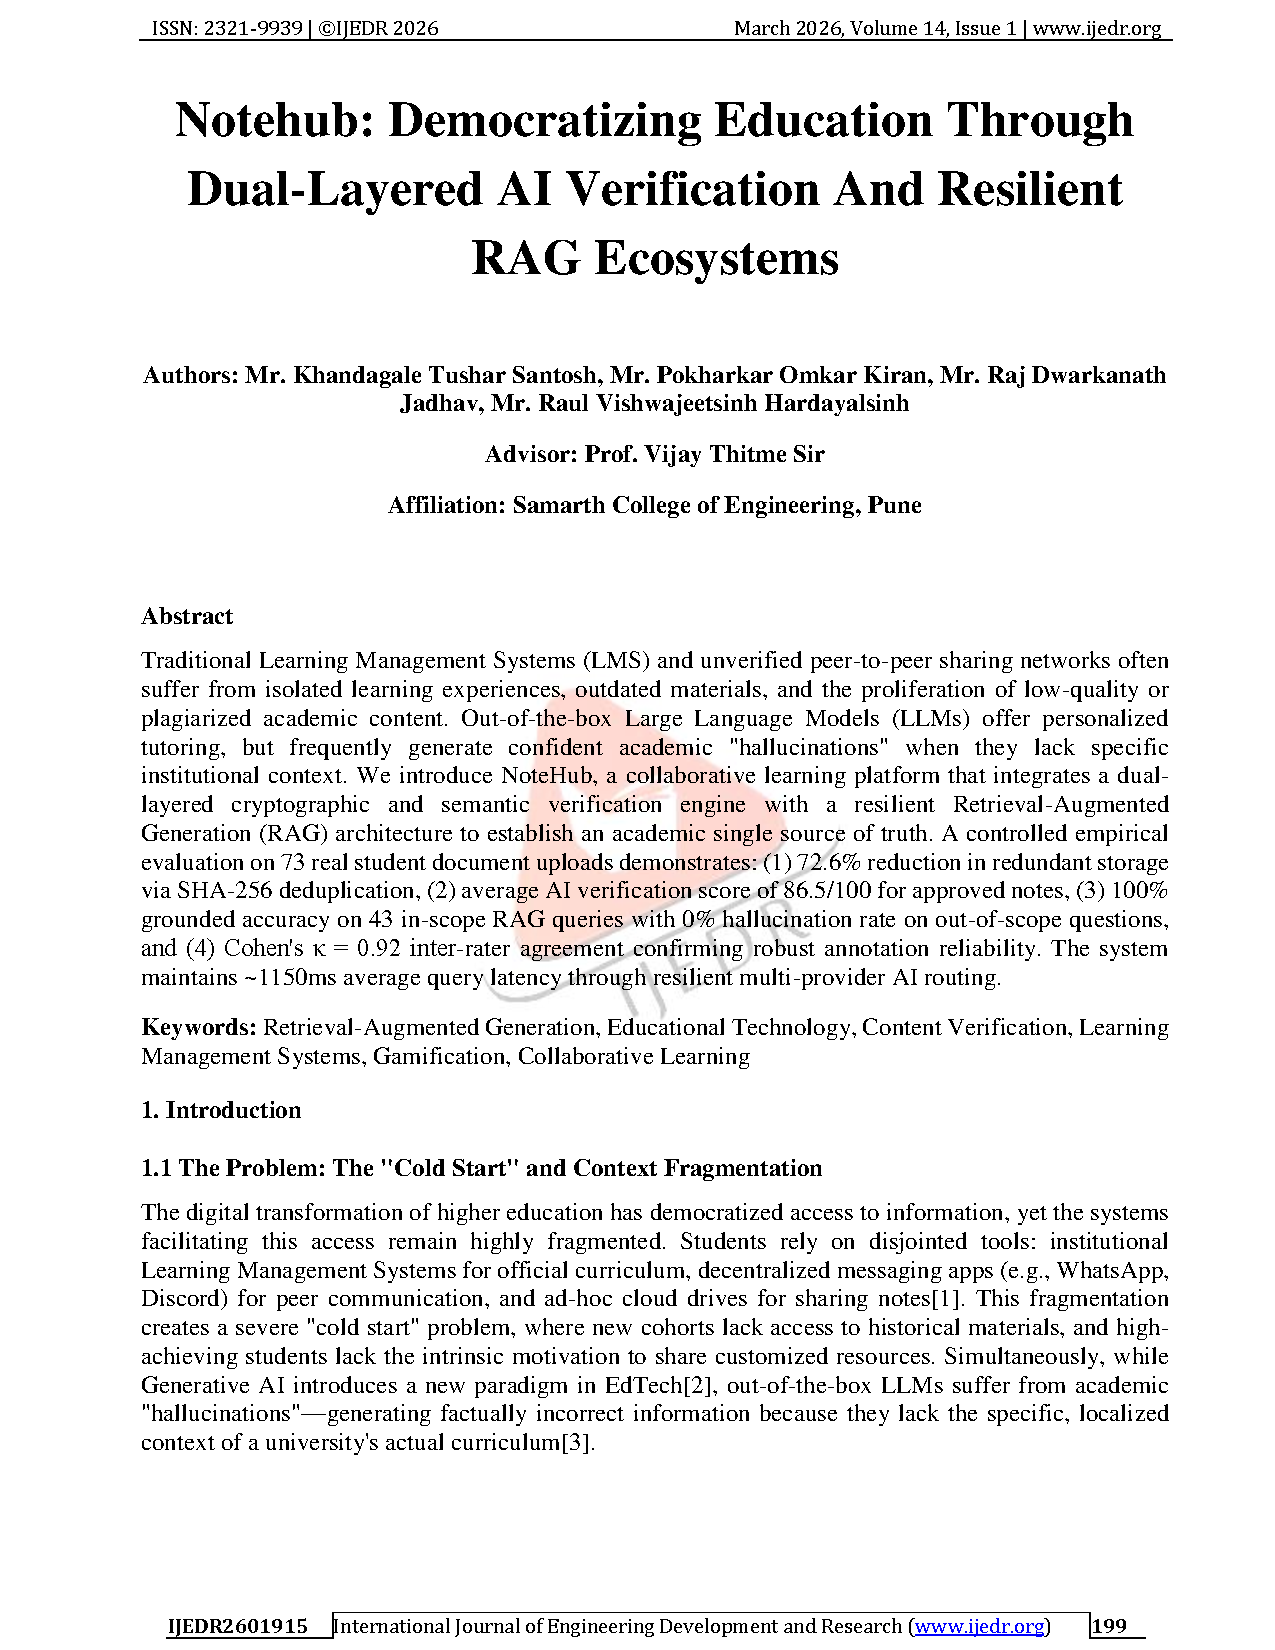
\includepdf[pages=1-8 , scale=0.9]{Published Paper.pdf}
\newpage
\section{CERTIFICATES}

\begin{figure}[H]
    \centering
    \includegraphics[width=0.75\linewidth]{Tushar.jpg}
    \caption{Khandagale Tushar Santosh}
    \label{fig:placeholder-1}
\end{figure}

\begin{figure}[H]
    \centering
    \includegraphics[width=0.75\linewidth]{Omkar.jpg}
    \caption{Pokharkar Omkar Kiran}
    \label{fig:placeholder-2}
\end{figure}

\begin{figure}[H]
    \centering
    \includegraphics[width=0.75\linewidth]{Raj.jpg}
    \caption{Raj Dwarkanath Jadhav}
    \label{fig:placeholder-3}
\end{figure}

\begin{figure}[H]
    \centering
    \includegraphics[width=0.75\linewidth]{Vishwajeet.jpg}
    \caption{Raul Vishwajeetsinh Hardayalsinh}
    \label{fig:placeholder-4}
\end{figure}
\chapter{PLAGIARISM REPORT}
\rule{\textwidth}{1pt}

\section{DETAILS OF PLAGIARISM REPORT :}

% \begin{enumerate}
%     \item \textbf{Report Title :} NOTEHUB: INTELLIGENT PLATFORM FOR STUDENT KNOWLEDGE SHARING\\
%     \item \textbf{Website :} \href{https://plagiarismdetector.net/}{https://plagiarismdetector.net/} \\
%     \item \textbf{Report Generated Date :} / /2026 \\
%     \item \textbf{Uniqueness:} \%  Plagiarised :\% Total Words: 1000\\
%     \item \textbf{Total Character: }7334
% \newpage
% \includepdf[pages=- , scale=0.9]{Plagiarism Report.pdf}
% \end{enumerate}
\end{document}